% Capitolul 7: Ipoteza piețelor eficiente, mersul aleator și testele VR
% Statistica piețelor financiare -- Program de licență, Academia de Studii Economice din București
% GENERAT de latex/build_chapter7.py -- modificați generatorul, nu acest fișier.

\newcommand{\coursename}{Statistica piețelor financiare}
\def\sfmlang{ro}
% Preambul comun SFM -- Statistica piețelor financiare / Statistics of Financial Markets (Beamer, 16:9)
% Același design ca MFM. Înainte de % Preambul comun SFM -- Statistica piețelor financiare / Statistics of Financial Markets (Beamer, 16:9)
% Același design ca MFM. Înainte de % Preambul comun SFM -- Statistica piețelor financiare / Statistics of Financial Markets (Beamer, 16:9)
% Același design ca MFM. Înainte de \input{../../latex/preamble} se definește
%   \newcommand{\coursename}{Statistics of Financial Markets}      (EN)
%   \newcommand{\coursename}{Statistica piețelor financiare}       (RO)  și  \def\sfmlang{ro}
% Fișierele .tex se află în EN/Courses, EN/Seminars, RO/Cursuri, RO/Seminarii (două niveluri sub rădăcină).
% Deck-urile sînt generate de latex/build_chapterN.py / build_seminarN.py (vezi latex/sfm_build.py).

\documentclass[9pt, aspectratio=169, t]{beamer}
\providecommand{\coursename}{Statistics of Financial Markets}

% Ensure content fits on slides
\setbeamersize{text margin left=8mm, text margin right=8mm}

%=============================================================================
% THEME AND STYLE CONFIGURATION
%=============================================================================
\usetheme{default}
% Using default theme for clean header/footer control

% Color Palette (matching Redispatch PDF)
\definecolor{MainBlue}{RGB}{26, 58, 110}
\definecolor{AccentBlue}{RGB}{26, 58, 110}
\definecolor{IDAred}{RGB}{205, 0, 0}
\definecolor{DarkGray}{RGB}{51, 51, 51}
\definecolor{MediumGray}{RGB}{128, 128, 128}
\definecolor{LightGray}{RGB}{248, 248, 248}
\definecolor{VeryLightGray}{RGB}{235, 235, 235}
\definecolor{KeynoteGray}{RGB}{218, 218, 218}
\definecolor{SectionGray}{RGB}{120, 120, 120}
\definecolor{FooterGray}{RGB}{100, 100, 100}
\definecolor{Crimson}{RGB}{220, 53, 69}
\definecolor{Forest}{RGB}{46, 125, 50}
\definecolor{Amber}{RGB}{181, 133, 63}
\definecolor{Orange}{RGB}{230, 126, 34}
\definecolor{Purple}{RGB}{142, 68, 173}

% Gradient background (exact Keynote 315° gradient: white to RGB 218,218,218)
\setbeamertemplate{background}{%
    \begin{tikzpicture}[remember picture, overlay]
        \shade[shading=axis, shading angle=315,
        top color=white, bottom color=KeynoteGray]
        (current page.south west) rectangle (current page.north east);
    \end{tikzpicture}%
}
% Fallback solid color for compatibility
\setbeamercolor{background canvas}{bg=}

\setbeamercolor{palette primary}{bg=MainBlue, fg=white}
\setbeamercolor{palette secondary}{bg=MainBlue!85, fg=white}
\setbeamercolor{palette tertiary}{bg=MainBlue!70, fg=white}
\setbeamercolor{structure}{fg=MainBlue}
\setbeamercolor{title}{fg=IDAred}
\setbeamercolor{frametitle}{fg=IDAred, bg=}
\setbeamercolor{block title}{bg=MainBlue, fg=white}
\setbeamercolor{block body}{bg=VeryLightGray, fg=DarkGray}
\setbeamercolor{block title alerted}{bg=Crimson, fg=white}
\setbeamercolor{block body alerted}{bg=Crimson!8, fg=DarkGray}
\setbeamercolor{block title example}{bg=Forest, fg=white}
\setbeamercolor{block body example}{bg=Forest!8, fg=DarkGray}
\setbeamercolor{item}{fg=MainBlue}

% Footer colors (override Madrid theme blue)
\setbeamercolor{author in head/foot}{fg=FooterGray, bg=}
\setbeamercolor{title in head/foot}{fg=FooterGray, bg=}
\setbeamercolor{date in head/foot}{fg=FooterGray, bg=}
\setbeamercolor{section in head/foot}{fg=FooterGray, bg=}
\setbeamercolor{subsection in head/foot}{fg=FooterGray, bg=}

% Bullet styles (apply everywhere including blocks)
\setbeamertemplate{itemize item}{\color{MainBlue}$\boxdot$}
\setbeamertemplate{itemize subitem}{\color{MainBlue}$\blacktriangleright$}
\setbeamertemplate{itemize subsubitem}{\color{MainBlue}\tiny$\bullet$}
\setbeamertemplate{itemize/enumerate body begin}{\normalsize}
\setbeamertemplate{itemize/enumerate subbody begin}{\normalsize}

% Item spacing - compact style
\setlength{\leftmargini}{10pt}       % Level 1: minimal indent
\setlength{\leftmarginii}{10pt}      % Level 2: minimal additional indent
% Compact list spacing (zero extra space before/after lists in blocks)
\makeatletter
\def\@listi{\leftmargin\leftmargini \topsep 0pt \parsep 0pt \itemsep 0pt}
\def\@listii{\leftmargin\leftmarginii \topsep 0pt \parsep 0pt \itemsep 0pt}
\makeatother

\setbeamertemplate{navigation symbols}{}

%=============================================================================
% CUSTOM HEADLINE
%=============================================================================
\setbeamertemplate{headline}{%
    \vskip10pt%
    \hbox to \paperwidth{%
        \hskip0.5cm%
        {\small\color{FooterGray}\renewcommand{\hyperlink}[2]{##2}\insertsectionhead}%
        \hfill%
        \textcolor{FooterGray}{\small\insertframenumber}%
        \hskip0.5cm%
    }%
    \vskip4pt%
    {\color{FooterGray}\hrule height 0.4pt}%
}

%=============================================================================
% CUSTOM FOOTER
%=============================================================================
\usepackage{fontawesome5}

\setbeamertemplate{footline}{%
    {\color{FooterGray}\hrule height 0.4pt}%
    \vskip4pt%
    \hbox to \paperwidth{%
        \hskip0.5cm%
        \textcolor{FooterGray}{\small\coursename}%
        \hfill%
        \raisebox{-0.1em}{%
            \begin{tikzpicture}[x=0.08em, y=0.08em, line width=0.4pt]
                \draw[FooterGray] (0,3) -- (1,4) -- (2,3.5) -- (3,5) -- (4,4) -- (5,6) -- (6,5.5) -- (7,4) -- (8,5) -- (9,7) -- (10,6) -- (11,5) -- (12,6.5) -- (13,8) -- (14,7) -- (15,6) -- (16,7.5) -- (17,9) -- (18,8) -- (19,7) -- (20,8.5) -- (21,10) -- (22,9) -- (23,8) -- (24,9.5);
            \end{tikzpicture}%
        }%
        \hskip0.5cm%
    }%
    \vskip6pt%
}

%=============================================================================
% PACKAGES
%=============================================================================
\usepackage[utf8]{inputenc}
\DeclareUnicodeCharacter{03B1}{\ensuremath{\alpha}}
\usepackage[T1]{fontenc}
\usepackage{amsmath, amssymb, amsthm}
\usepackage{mathtools}
\usepackage{bm}
\usepackage{tikz}
\usetikzlibrary{arrows.meta, positioning, shapes, calc, decorations.pathreplacing, shadings}
\usepackage{booktabs}
\usepackage{multirow}
\usepackage{array}
\usepackage{graphicx}
\usepackage{hyperref}
\usepackage{colortbl}
\usepackage{listings}
\lstset{language=Python, basicstyle=\ttfamily\scriptsize, keywordstyle=\color{MainBlue}\bfseries,
  commentstyle=\color{Forest}, stringstyle=\color{Crimson}, breaklines=true,
  frame=none, backgroundcolor=\color{VeryLightGray}, xleftmargin=2mm}
\hypersetup{colorlinks=true, linkcolor=MainBlue, urlcolor=MainBlue}
\graphicspath{{../../logos/}{../../charts/}{../../photos/}}
\usepackage{xcolor}
\hfuzz=2pt  % Suppress tiny overfull warnings (<2pt)
\vfuzz=2pt  % Suppress tiny vertical overfull warnings (<2pt)

%=============================================================================
% QUANTLET COMMANDS
%   \quantlet{<displayed name>}{<url>}       (generic, compatible with the older SFM decks)
%   \sfmquantlet{Ch_05}{SFM_ch5_garch}       -> https://github.com/danpele/SFM/tree/main/Quantlets/Ch_05/SFM_ch5_garch
%   \qlurl{<folder>} is defined per chapter by the generator (Quantlets/Ch_NN/<folder>)
%=============================================================================
\newcommand{\sfmrepo}{https://github.com/danpele/SFM}
\newcommand{\sfmqlbase}{https://github.com/danpele/SFM/tree/main/Quantlets}
\newcommand{\quantlet}[2]{%
    \hfill\href{#2}{%
        \raisebox{-0.15em}{
\includegraphics[height=0.7em]{ql_logo.png}}%
        \textcolor{MainBlue}{\tiny\ #1}%
    }%
}
\newcommand{\sfmquantlet}[2]{\quantlet{\detokenize{#2}}{\sfmqlbase/#1/#2}}

%=============================================================================
% NOTEBOOKS (Google Colab)
%   \colaburl{notebooks/EN/chapter5_seminar_notebook.ipynb} -> the Colab link of a file in the SFM repo
%   \nb: the chapter notebook (each seminar deck redefines it with \renewcommand)
%=============================================================================
\newcommand{\colaburl}[1]{https://colab.research.google.com/github/danpele/SFM/blob/main/#1}
\newcommand{\nb}{https://colab.research.google.com/github/danpele/SFM/tree/main/notebooks/EN}
\newcommand{\nbname}{notebooks/EN}

%=============================================================================
% SLIDE HELPERS (used by the generators; the same as in MFM)
%=============================================================================
% local font size for list bodies (the preamble forces \normalsize)
\newcommand{\itemsize}[1]{\setbeamertemplate{itemize/enumerate body begin}{#1}\setbeamertemplate{itemize/enumerate subbody begin}{#1}}
\newcommand{\intitle}[1]{{\hypersetup{urlcolor=white}#1}}   % white links inside coloured title bars
\newcommand{\imgcap}[1]{{\scriptsize #1}\\[0.5mm]}          % caption under a photo
\newcommand{\imgcredit}[2]{{\tiny\color{FooterGray}\href{#1}{#2}}}   % image credit: source URL, author/licence
\newcommand{\aiprompt}[1]{{\ttfamily\color{MainBlue}#1}}     % a prompt to an AI assistant

%=============================================================================
% SEMINARS: student version by default; the instructor wrapper *_solutions.tex sets \solutionstrue
%=============================================================================
\makeatletter\@ifundefined{ifsolutions}{\expandafter\newif\csname ifsolutions\endcsname}{}\makeatother
\newcommand{\solonly}[1]{\ifsolutions #1\fi}
\newcommand{\propsub}{\ifsolutions\else\framesubtitle{\ifdefined\sfmlang Rezolvarea se discută la seminar\else Solution discussed in class\fi}\fi}

%=============================================================================
% APPENDIX AND CHAPTER LINKS (latex/appendix_links.py writes the calls; it also re-declares these
% macros before \begin{document}, so the decks compile with or without this preamble block)
%=============================================================================
\providecommand{\sfmapplink}[3]{\hypertarget{#2}{}\hyperlink{#1}{\beamergotobutton{#3}}}
\providecommand{\sfmappback}[2]{\begin{tikzpicture}[remember picture,overlay]\node[anchor=south east] at ([xshift=-3mm,yshift=7mm]current page.south east){\hyperlink{#1}{\beamerreturnbutton{#2}}};\end{tikzpicture}}
\providecommand{\sfmchlink}[2]{\href{#1}{#2}}
\providecommand{\sfmchlinkt}[2]{\href{#1}{\usebeamercolor[fg]{frametitle}#2}}

%=============================================================================
% QUANTINAR COMMAND: link către un curs Quantinar (subiecte avansate)
%=============================================================================
\newcommand{\quantinar}[2]{%
    \href{#2}{%
        \raisebox{-0.15em}{
\includegraphics[height=0.8em]{qr_logo.png}}%
        \textcolor{MainBlue}{\scriptsize\ #1}%
    }%
}

%=============================================================================
% CUSTOM TITLE PAGE
%=============================================================================
\defbeamertemplate*{title page}{hybrid}[1][]
{
    \vspace{0.2cm}
    % Logos row - top header (with clickable links)
    \begin{center}
        \href{https://www.ase.ro}{
\includegraphics[height=1.0cm]{ase_logo.png}}\hspace{0.3cm}%
        \href{https://theida.net}{
\includegraphics[height=1.0cm]{ida_logo.png}}\hspace{0.3cm}%
        \href{https://blockchain-research-center.com}{
\includegraphics[height=1.0cm]{brc_logo.png}}\hspace{0.3cm}%
        \href{https://www.ai4efin.ase.ro}{
\includegraphics[height=1.0cm]{ai4efin_logo.png}}\hspace{0.3cm}%
        \href{https://ipe.ro/new}{
\includegraphics[height=1.0cm]{acad_logo.png}}\hspace{0.3cm}%
        \href{https://www.digital-finance-msca.com}{
\includegraphics[height=1.0cm]{msca_logo.png}}%
    \end{center}

    \vspace{0.6cm}

    % Main title with Q logos on sides (with clickable links)
    \begin{center}
        \begin{minipage}{0.1\textwidth}
            \centering
            \href{https://quantlet.com}{
\includegraphics[height=1.1cm]{ql_logo.png}}
        \end{minipage}%
        \begin{minipage}{0.78\textwidth}
            \centering
            {\LARGE\bfseries\usebeamercolor[fg]{title}\inserttitle}

            \vspace{0.3cm}

            {\usebeamerfont{subtitle}\usebeamercolor[fg]{title}\insertsubtitle}
        \end{minipage}%
        \begin{minipage}{0.1\textwidth}
            \centering
            \href{https://quantinar.com}{
\includegraphics[height=1.1cm]{qr_logo.png}}
        \end{minipage}
    \end{center}

    \vspace{0.6cm}

    % Authors (left aligned)
    \hspace{0.5cm}{\usebeamerfont{author}\insertauthor}

    \vspace{0.3cm}

    % Institute/Affiliations (left aligned)
    \hspace{0.5cm}\begin{minipage}[t]{0.9\textwidth}
        \raggedright\small\insertinstitute
    \end{minipage}
}

%=============================================================================
% THEOREM ENVIRONMENTS
%=============================================================================
\theoremstyle{definition}
\setbeamertemplate{theorems}[numbered]
\ifdefined\sfmlang
\newtheorem{defn}{Definiție}
\newtheorem{thm}{Teoremă}
\newtheorem{prop}{Propoziție}
\newtheorem{rmk}{Observație}
\else
\newtheorem{defn}{Definition}
\newtheorem{thm}{Theorem}
\newtheorem{prop}{Proposition}
\newtheorem{rmk}{Remark}
\fi

%=============================================================================
% CENTRED MINIPAGE (no extra vertical space)
%=============================================================================
\newenvironment{cminipage}[1]{%
    \par\noindent\hfill\begin{minipage}{#1}\ignorespaces
}{%
    \end{minipage}\hfill\null\par
}

%=============================================================================
% CUSTOM COMMANDS
%=============================================================================
\newcommand{\E}{\mathbb{E}}
\newcommand{\Var}{\text{Var}}
\newcommand{\Cov}{\text{Cov}}
\newcommand{\Corr}{\text{Corr}}
\newcommand{\R}{\mathbb{R}}
\newcommand{\N}{\mathbb{N}}
\newcommand{\Z}{\mathbb{Z}}
\newcommand{\B}{\mathbf{B}}
\newcommand{\imark}{\textcolor{MainBlue}{\textbullet}}
\newcommand{\RMSE}{\text{RMSE}}
\newcommand{\MAE}{\text{MAE}}
\newcommand{\MAPE}{\text{MAPE}}

 se definește
%   \newcommand{\coursename}{Statistics of Financial Markets}      (EN)
%   \newcommand{\coursename}{Statistica piețelor financiare}       (RO)  și  \def\sfmlang{ro}
% Fișierele .tex se află în EN/Courses, EN/Seminars, RO/Cursuri, RO/Seminarii (două niveluri sub rădăcină).
% Deck-urile sînt generate de latex/build_chapterN.py / build_seminarN.py (vezi latex/sfm_build.py).

\documentclass[9pt, aspectratio=169, t]{beamer}
\providecommand{\coursename}{Statistics of Financial Markets}

% Ensure content fits on slides
\setbeamersize{text margin left=8mm, text margin right=8mm}

%=============================================================================
% THEME AND STYLE CONFIGURATION
%=============================================================================
\usetheme{default}
% Using default theme for clean header/footer control

% Color Palette (matching Redispatch PDF)
\definecolor{MainBlue}{RGB}{26, 58, 110}
\definecolor{AccentBlue}{RGB}{26, 58, 110}
\definecolor{IDAred}{RGB}{205, 0, 0}
\definecolor{DarkGray}{RGB}{51, 51, 51}
\definecolor{MediumGray}{RGB}{128, 128, 128}
\definecolor{LightGray}{RGB}{248, 248, 248}
\definecolor{VeryLightGray}{RGB}{235, 235, 235}
\definecolor{KeynoteGray}{RGB}{218, 218, 218}
\definecolor{SectionGray}{RGB}{120, 120, 120}
\definecolor{FooterGray}{RGB}{100, 100, 100}
\definecolor{Crimson}{RGB}{220, 53, 69}
\definecolor{Forest}{RGB}{46, 125, 50}
\definecolor{Amber}{RGB}{181, 133, 63}
\definecolor{Orange}{RGB}{230, 126, 34}
\definecolor{Purple}{RGB}{142, 68, 173}

% Gradient background (exact Keynote 315° gradient: white to RGB 218,218,218)
\setbeamertemplate{background}{%
    \begin{tikzpicture}[remember picture, overlay]
        \shade[shading=axis, shading angle=315,
        top color=white, bottom color=KeynoteGray]
        (current page.south west) rectangle (current page.north east);
    \end{tikzpicture}%
}
% Fallback solid color for compatibility
\setbeamercolor{background canvas}{bg=}

\setbeamercolor{palette primary}{bg=MainBlue, fg=white}
\setbeamercolor{palette secondary}{bg=MainBlue!85, fg=white}
\setbeamercolor{palette tertiary}{bg=MainBlue!70, fg=white}
\setbeamercolor{structure}{fg=MainBlue}
\setbeamercolor{title}{fg=IDAred}
\setbeamercolor{frametitle}{fg=IDAred, bg=}
\setbeamercolor{block title}{bg=MainBlue, fg=white}
\setbeamercolor{block body}{bg=VeryLightGray, fg=DarkGray}
\setbeamercolor{block title alerted}{bg=Crimson, fg=white}
\setbeamercolor{block body alerted}{bg=Crimson!8, fg=DarkGray}
\setbeamercolor{block title example}{bg=Forest, fg=white}
\setbeamercolor{block body example}{bg=Forest!8, fg=DarkGray}
\setbeamercolor{item}{fg=MainBlue}

% Footer colors (override Madrid theme blue)
\setbeamercolor{author in head/foot}{fg=FooterGray, bg=}
\setbeamercolor{title in head/foot}{fg=FooterGray, bg=}
\setbeamercolor{date in head/foot}{fg=FooterGray, bg=}
\setbeamercolor{section in head/foot}{fg=FooterGray, bg=}
\setbeamercolor{subsection in head/foot}{fg=FooterGray, bg=}

% Bullet styles (apply everywhere including blocks)
\setbeamertemplate{itemize item}{\color{MainBlue}$\boxdot$}
\setbeamertemplate{itemize subitem}{\color{MainBlue}$\blacktriangleright$}
\setbeamertemplate{itemize subsubitem}{\color{MainBlue}\tiny$\bullet$}
\setbeamertemplate{itemize/enumerate body begin}{\normalsize}
\setbeamertemplate{itemize/enumerate subbody begin}{\normalsize}

% Item spacing - compact style
\setlength{\leftmargini}{10pt}       % Level 1: minimal indent
\setlength{\leftmarginii}{10pt}      % Level 2: minimal additional indent
% Compact list spacing (zero extra space before/after lists in blocks)
\makeatletter
\def\@listi{\leftmargin\leftmargini \topsep 0pt \parsep 0pt \itemsep 0pt}
\def\@listii{\leftmargin\leftmarginii \topsep 0pt \parsep 0pt \itemsep 0pt}
\makeatother

\setbeamertemplate{navigation symbols}{}

%=============================================================================
% CUSTOM HEADLINE
%=============================================================================
\setbeamertemplate{headline}{%
    \vskip10pt%
    \hbox to \paperwidth{%
        \hskip0.5cm%
        {\small\color{FooterGray}\renewcommand{\hyperlink}[2]{##2}\insertsectionhead}%
        \hfill%
        \textcolor{FooterGray}{\small\insertframenumber}%
        \hskip0.5cm%
    }%
    \vskip4pt%
    {\color{FooterGray}\hrule height 0.4pt}%
}

%=============================================================================
% CUSTOM FOOTER
%=============================================================================
\usepackage{fontawesome5}

\setbeamertemplate{footline}{%
    {\color{FooterGray}\hrule height 0.4pt}%
    \vskip4pt%
    \hbox to \paperwidth{%
        \hskip0.5cm%
        \textcolor{FooterGray}{\small\coursename}%
        \hfill%
        \raisebox{-0.1em}{%
            \begin{tikzpicture}[x=0.08em, y=0.08em, line width=0.4pt]
                \draw[FooterGray] (0,3) -- (1,4) -- (2,3.5) -- (3,5) -- (4,4) -- (5,6) -- (6,5.5) -- (7,4) -- (8,5) -- (9,7) -- (10,6) -- (11,5) -- (12,6.5) -- (13,8) -- (14,7) -- (15,6) -- (16,7.5) -- (17,9) -- (18,8) -- (19,7) -- (20,8.5) -- (21,10) -- (22,9) -- (23,8) -- (24,9.5);
            \end{tikzpicture}%
        }%
        \hskip0.5cm%
    }%
    \vskip6pt%
}

%=============================================================================
% PACKAGES
%=============================================================================
\usepackage[utf8]{inputenc}
\DeclareUnicodeCharacter{03B1}{\ensuremath{\alpha}}
\usepackage[T1]{fontenc}
\usepackage{amsmath, amssymb, amsthm}
\usepackage{mathtools}
\usepackage{bm}
\usepackage{tikz}
\usetikzlibrary{arrows.meta, positioning, shapes, calc, decorations.pathreplacing, shadings}
\usepackage{booktabs}
\usepackage{multirow}
\usepackage{array}
\usepackage{graphicx}
\usepackage{hyperref}
\usepackage{colortbl}
\usepackage{listings}
\lstset{language=Python, basicstyle=\ttfamily\scriptsize, keywordstyle=\color{MainBlue}\bfseries,
  commentstyle=\color{Forest}, stringstyle=\color{Crimson}, breaklines=true,
  frame=none, backgroundcolor=\color{VeryLightGray}, xleftmargin=2mm}
\hypersetup{colorlinks=true, linkcolor=MainBlue, urlcolor=MainBlue}
\graphicspath{{../../logos/}{../../charts/}{../../photos/}}
\usepackage{xcolor}
\hfuzz=2pt  % Suppress tiny overfull warnings (<2pt)
\vfuzz=2pt  % Suppress tiny vertical overfull warnings (<2pt)

%=============================================================================
% QUANTLET COMMANDS
%   \quantlet{<displayed name>}{<url>}       (generic, compatible with the older SFM decks)
%   \sfmquantlet{Ch_05}{SFM_ch5_garch}       -> https://github.com/danpele/SFM/tree/main/Quantlets/Ch_05/SFM_ch5_garch
%   \qlurl{<folder>} is defined per chapter by the generator (Quantlets/Ch_NN/<folder>)
%=============================================================================
\newcommand{\sfmrepo}{https://github.com/danpele/SFM}
\newcommand{\sfmqlbase}{https://github.com/danpele/SFM/tree/main/Quantlets}
\newcommand{\quantlet}[2]{%
    \hfill\href{#2}{%
        \raisebox{-0.15em}{
\includegraphics[height=0.7em]{ql_logo.png}}%
        \textcolor{MainBlue}{\tiny\ #1}%
    }%
}
\newcommand{\sfmquantlet}[2]{\quantlet{\detokenize{#2}}{\sfmqlbase/#1/#2}}

%=============================================================================
% NOTEBOOKS (Google Colab)
%   \colaburl{notebooks/EN/chapter5_seminar_notebook.ipynb} -> the Colab link of a file in the SFM repo
%   \nb: the chapter notebook (each seminar deck redefines it with \renewcommand)
%=============================================================================
\newcommand{\colaburl}[1]{https://colab.research.google.com/github/danpele/SFM/blob/main/#1}
\newcommand{\nb}{https://colab.research.google.com/github/danpele/SFM/tree/main/notebooks/EN}
\newcommand{\nbname}{notebooks/EN}

%=============================================================================
% SLIDE HELPERS (used by the generators; the same as in MFM)
%=============================================================================
% local font size for list bodies (the preamble forces \normalsize)
\newcommand{\itemsize}[1]{\setbeamertemplate{itemize/enumerate body begin}{#1}\setbeamertemplate{itemize/enumerate subbody begin}{#1}}
\newcommand{\intitle}[1]{{\hypersetup{urlcolor=white}#1}}   % white links inside coloured title bars
\newcommand{\imgcap}[1]{{\scriptsize #1}\\[0.5mm]}          % caption under a photo
\newcommand{\imgcredit}[2]{{\tiny\color{FooterGray}\href{#1}{#2}}}   % image credit: source URL, author/licence
\newcommand{\aiprompt}[1]{{\ttfamily\color{MainBlue}#1}}     % a prompt to an AI assistant

%=============================================================================
% SEMINARS: student version by default; the instructor wrapper *_solutions.tex sets \solutionstrue
%=============================================================================
\makeatletter\@ifundefined{ifsolutions}{\expandafter\newif\csname ifsolutions\endcsname}{}\makeatother
\newcommand{\solonly}[1]{\ifsolutions #1\fi}
\newcommand{\propsub}{\ifsolutions\else\framesubtitle{\ifdefined\sfmlang Rezolvarea se discută la seminar\else Solution discussed in class\fi}\fi}

%=============================================================================
% APPENDIX AND CHAPTER LINKS (latex/appendix_links.py writes the calls; it also re-declares these
% macros before \begin{document}, so the decks compile with or without this preamble block)
%=============================================================================
\providecommand{\sfmapplink}[3]{\hypertarget{#2}{}\hyperlink{#1}{\beamergotobutton{#3}}}
\providecommand{\sfmappback}[2]{\begin{tikzpicture}[remember picture,overlay]\node[anchor=south east] at ([xshift=-3mm,yshift=7mm]current page.south east){\hyperlink{#1}{\beamerreturnbutton{#2}}};\end{tikzpicture}}
\providecommand{\sfmchlink}[2]{\href{#1}{#2}}
\providecommand{\sfmchlinkt}[2]{\href{#1}{\usebeamercolor[fg]{frametitle}#2}}

%=============================================================================
% QUANTINAR COMMAND: link către un curs Quantinar (subiecte avansate)
%=============================================================================
\newcommand{\quantinar}[2]{%
    \href{#2}{%
        \raisebox{-0.15em}{
\includegraphics[height=0.8em]{qr_logo.png}}%
        \textcolor{MainBlue}{\scriptsize\ #1}%
    }%
}

%=============================================================================
% CUSTOM TITLE PAGE
%=============================================================================
\defbeamertemplate*{title page}{hybrid}[1][]
{
    \vspace{0.2cm}
    % Logos row - top header (with clickable links)
    \begin{center}
        \href{https://www.ase.ro}{
\includegraphics[height=1.0cm]{ase_logo.png}}\hspace{0.3cm}%
        \href{https://theida.net}{
\includegraphics[height=1.0cm]{ida_logo.png}}\hspace{0.3cm}%
        \href{https://blockchain-research-center.com}{
\includegraphics[height=1.0cm]{brc_logo.png}}\hspace{0.3cm}%
        \href{https://www.ai4efin.ase.ro}{
\includegraphics[height=1.0cm]{ai4efin_logo.png}}\hspace{0.3cm}%
        \href{https://ipe.ro/new}{
\includegraphics[height=1.0cm]{acad_logo.png}}\hspace{0.3cm}%
        \href{https://www.digital-finance-msca.com}{
\includegraphics[height=1.0cm]{msca_logo.png}}%
    \end{center}

    \vspace{0.6cm}

    % Main title with Q logos on sides (with clickable links)
    \begin{center}
        \begin{minipage}{0.1\textwidth}
            \centering
            \href{https://quantlet.com}{
\includegraphics[height=1.1cm]{ql_logo.png}}
        \end{minipage}%
        \begin{minipage}{0.78\textwidth}
            \centering
            {\LARGE\bfseries\usebeamercolor[fg]{title}\inserttitle}

            \vspace{0.3cm}

            {\usebeamerfont{subtitle}\usebeamercolor[fg]{title}\insertsubtitle}
        \end{minipage}%
        \begin{minipage}{0.1\textwidth}
            \centering
            \href{https://quantinar.com}{
\includegraphics[height=1.1cm]{qr_logo.png}}
        \end{minipage}
    \end{center}

    \vspace{0.6cm}

    % Authors (left aligned)
    \hspace{0.5cm}{\usebeamerfont{author}\insertauthor}

    \vspace{0.3cm}

    % Institute/Affiliations (left aligned)
    \hspace{0.5cm}\begin{minipage}[t]{0.9\textwidth}
        \raggedright\small\insertinstitute
    \end{minipage}
}

%=============================================================================
% THEOREM ENVIRONMENTS
%=============================================================================
\theoremstyle{definition}
\setbeamertemplate{theorems}[numbered]
\ifdefined\sfmlang
\newtheorem{defn}{Definiție}
\newtheorem{thm}{Teoremă}
\newtheorem{prop}{Propoziție}
\newtheorem{rmk}{Observație}
\else
\newtheorem{defn}{Definition}
\newtheorem{thm}{Theorem}
\newtheorem{prop}{Proposition}
\newtheorem{rmk}{Remark}
\fi

%=============================================================================
% CENTRED MINIPAGE (no extra vertical space)
%=============================================================================
\newenvironment{cminipage}[1]{%
    \par\noindent\hfill\begin{minipage}{#1}\ignorespaces
}{%
    \end{minipage}\hfill\null\par
}

%=============================================================================
% CUSTOM COMMANDS
%=============================================================================
\newcommand{\E}{\mathbb{E}}
\newcommand{\Var}{\text{Var}}
\newcommand{\Cov}{\text{Cov}}
\newcommand{\Corr}{\text{Corr}}
\newcommand{\R}{\mathbb{R}}
\newcommand{\N}{\mathbb{N}}
\newcommand{\Z}{\mathbb{Z}}
\newcommand{\B}{\mathbf{B}}
\newcommand{\imark}{\textcolor{MainBlue}{\textbullet}}
\newcommand{\RMSE}{\text{RMSE}}
\newcommand{\MAE}{\text{MAE}}
\newcommand{\MAPE}{\text{MAPE}}

 se definește
%   \newcommand{\coursename}{Statistics of Financial Markets}      (EN)
%   \newcommand{\coursename}{Statistica piețelor financiare}       (RO)  și  \def\sfmlang{ro}
% Fișierele .tex se află în EN/Courses, EN/Seminars, RO/Cursuri, RO/Seminarii (două niveluri sub rădăcină).
% Deck-urile sînt generate de latex/build_chapterN.py / build_seminarN.py (vezi latex/sfm_build.py).

\documentclass[9pt, aspectratio=169, t]{beamer}
\providecommand{\coursename}{Statistics of Financial Markets}

% Ensure content fits on slides
\setbeamersize{text margin left=8mm, text margin right=8mm}

%=============================================================================
% THEME AND STYLE CONFIGURATION
%=============================================================================
\usetheme{default}
% Using default theme for clean header/footer control

% Color Palette (matching Redispatch PDF)
\definecolor{MainBlue}{RGB}{26, 58, 110}
\definecolor{AccentBlue}{RGB}{26, 58, 110}
\definecolor{IDAred}{RGB}{205, 0, 0}
\definecolor{DarkGray}{RGB}{51, 51, 51}
\definecolor{MediumGray}{RGB}{128, 128, 128}
\definecolor{LightGray}{RGB}{248, 248, 248}
\definecolor{VeryLightGray}{RGB}{235, 235, 235}
\definecolor{KeynoteGray}{RGB}{218, 218, 218}
\definecolor{SectionGray}{RGB}{120, 120, 120}
\definecolor{FooterGray}{RGB}{100, 100, 100}
\definecolor{Crimson}{RGB}{220, 53, 69}
\definecolor{Forest}{RGB}{46, 125, 50}
\definecolor{Amber}{RGB}{181, 133, 63}
\definecolor{Orange}{RGB}{230, 126, 34}
\definecolor{Purple}{RGB}{142, 68, 173}

% Gradient background (exact Keynote 315° gradient: white to RGB 218,218,218)
\setbeamertemplate{background}{%
    \begin{tikzpicture}[remember picture, overlay]
        \shade[shading=axis, shading angle=315,
        top color=white, bottom color=KeynoteGray]
        (current page.south west) rectangle (current page.north east);
    \end{tikzpicture}%
}
% Fallback solid color for compatibility
\setbeamercolor{background canvas}{bg=}

\setbeamercolor{palette primary}{bg=MainBlue, fg=white}
\setbeamercolor{palette secondary}{bg=MainBlue!85, fg=white}
\setbeamercolor{palette tertiary}{bg=MainBlue!70, fg=white}
\setbeamercolor{structure}{fg=MainBlue}
\setbeamercolor{title}{fg=IDAred}
\setbeamercolor{frametitle}{fg=IDAred, bg=}
\setbeamercolor{block title}{bg=MainBlue, fg=white}
\setbeamercolor{block body}{bg=VeryLightGray, fg=DarkGray}
\setbeamercolor{block title alerted}{bg=Crimson, fg=white}
\setbeamercolor{block body alerted}{bg=Crimson!8, fg=DarkGray}
\setbeamercolor{block title example}{bg=Forest, fg=white}
\setbeamercolor{block body example}{bg=Forest!8, fg=DarkGray}
\setbeamercolor{item}{fg=MainBlue}

% Footer colors (override Madrid theme blue)
\setbeamercolor{author in head/foot}{fg=FooterGray, bg=}
\setbeamercolor{title in head/foot}{fg=FooterGray, bg=}
\setbeamercolor{date in head/foot}{fg=FooterGray, bg=}
\setbeamercolor{section in head/foot}{fg=FooterGray, bg=}
\setbeamercolor{subsection in head/foot}{fg=FooterGray, bg=}

% Bullet styles (apply everywhere including blocks)
\setbeamertemplate{itemize item}{\color{MainBlue}$\boxdot$}
\setbeamertemplate{itemize subitem}{\color{MainBlue}$\blacktriangleright$}
\setbeamertemplate{itemize subsubitem}{\color{MainBlue}\tiny$\bullet$}
\setbeamertemplate{itemize/enumerate body begin}{\normalsize}
\setbeamertemplate{itemize/enumerate subbody begin}{\normalsize}

% Item spacing - compact style
\setlength{\leftmargini}{10pt}       % Level 1: minimal indent
\setlength{\leftmarginii}{10pt}      % Level 2: minimal additional indent
% Compact list spacing (zero extra space before/after lists in blocks)
\makeatletter
\def\@listi{\leftmargin\leftmargini \topsep 0pt \parsep 0pt \itemsep 0pt}
\def\@listii{\leftmargin\leftmarginii \topsep 0pt \parsep 0pt \itemsep 0pt}
\makeatother

\setbeamertemplate{navigation symbols}{}

%=============================================================================
% CUSTOM HEADLINE
%=============================================================================
\setbeamertemplate{headline}{%
    \vskip10pt%
    \hbox to \paperwidth{%
        \hskip0.5cm%
        {\small\color{FooterGray}\renewcommand{\hyperlink}[2]{##2}\insertsectionhead}%
        \hfill%
        \textcolor{FooterGray}{\small\insertframenumber}%
        \hskip0.5cm%
    }%
    \vskip4pt%
    {\color{FooterGray}\hrule height 0.4pt}%
}

%=============================================================================
% CUSTOM FOOTER
%=============================================================================
\usepackage{fontawesome5}

\setbeamertemplate{footline}{%
    {\color{FooterGray}\hrule height 0.4pt}%
    \vskip4pt%
    \hbox to \paperwidth{%
        \hskip0.5cm%
        \textcolor{FooterGray}{\small\coursename}%
        \hfill%
        \raisebox{-0.1em}{%
            \begin{tikzpicture}[x=0.08em, y=0.08em, line width=0.4pt]
                \draw[FooterGray] (0,3) -- (1,4) -- (2,3.5) -- (3,5) -- (4,4) -- (5,6) -- (6,5.5) -- (7,4) -- (8,5) -- (9,7) -- (10,6) -- (11,5) -- (12,6.5) -- (13,8) -- (14,7) -- (15,6) -- (16,7.5) -- (17,9) -- (18,8) -- (19,7) -- (20,8.5) -- (21,10) -- (22,9) -- (23,8) -- (24,9.5);
            \end{tikzpicture}%
        }%
        \hskip0.5cm%
    }%
    \vskip6pt%
}

%=============================================================================
% PACKAGES
%=============================================================================
\usepackage[utf8]{inputenc}
\DeclareUnicodeCharacter{03B1}{\ensuremath{\alpha}}
\usepackage[T1]{fontenc}
\usepackage{amsmath, amssymb, amsthm}
\usepackage{mathtools}
\usepackage{bm}
\usepackage{tikz}
\usetikzlibrary{arrows.meta, positioning, shapes, calc, decorations.pathreplacing, shadings}
\usepackage{booktabs}
\usepackage{multirow}
\usepackage{array}
\usepackage{graphicx}
\usepackage{hyperref}
\usepackage{colortbl}
\usepackage{listings}
\lstset{language=Python, basicstyle=\ttfamily\scriptsize, keywordstyle=\color{MainBlue}\bfseries,
  commentstyle=\color{Forest}, stringstyle=\color{Crimson}, breaklines=true,
  frame=none, backgroundcolor=\color{VeryLightGray}, xleftmargin=2mm}
\hypersetup{colorlinks=true, linkcolor=MainBlue, urlcolor=MainBlue}
\graphicspath{{../../logos/}{../../charts/}{../../photos/}}
\usepackage{xcolor}
\hfuzz=2pt  % Suppress tiny overfull warnings (<2pt)
\vfuzz=2pt  % Suppress tiny vertical overfull warnings (<2pt)

%=============================================================================
% QUANTLET COMMANDS
%   \quantlet{<displayed name>}{<url>}       (generic, compatible with the older SFM decks)
%   \sfmquantlet{Ch_05}{SFM_ch5_garch}       -> https://github.com/danpele/SFM/tree/main/Quantlets/Ch_05/SFM_ch5_garch
%   \qlurl{<folder>} is defined per chapter by the generator (Quantlets/Ch_NN/<folder>)
%=============================================================================
\newcommand{\sfmrepo}{https://github.com/danpele/SFM}
\newcommand{\sfmqlbase}{https://github.com/danpele/SFM/tree/main/Quantlets}
\newcommand{\quantlet}[2]{%
    \hfill\href{#2}{%
        \raisebox{-0.15em}{
\includegraphics[height=0.7em]{ql_logo.png}}%
        \textcolor{MainBlue}{\tiny\ #1}%
    }%
}
\newcommand{\sfmquantlet}[2]{\quantlet{\detokenize{#2}}{\sfmqlbase/#1/#2}}

%=============================================================================
% NOTEBOOKS (Google Colab)
%   \colaburl{notebooks/EN/chapter5_seminar_notebook.ipynb} -> the Colab link of a file in the SFM repo
%   \nb: the chapter notebook (each seminar deck redefines it with \renewcommand)
%=============================================================================
\newcommand{\colaburl}[1]{https://colab.research.google.com/github/danpele/SFM/blob/main/#1}
\newcommand{\nb}{https://colab.research.google.com/github/danpele/SFM/tree/main/notebooks/EN}
\newcommand{\nbname}{notebooks/EN}

%=============================================================================
% SLIDE HELPERS (used by the generators; the same as in MFM)
%=============================================================================
% local font size for list bodies (the preamble forces \normalsize)
\newcommand{\itemsize}[1]{\setbeamertemplate{itemize/enumerate body begin}{#1}\setbeamertemplate{itemize/enumerate subbody begin}{#1}}
\newcommand{\intitle}[1]{{\hypersetup{urlcolor=white}#1}}   % white links inside coloured title bars
\newcommand{\imgcap}[1]{{\scriptsize #1}\\[0.5mm]}          % caption under a photo
\newcommand{\imgcredit}[2]{{\tiny\color{FooterGray}\href{#1}{#2}}}   % image credit: source URL, author/licence
\newcommand{\aiprompt}[1]{{\ttfamily\color{MainBlue}#1}}     % a prompt to an AI assistant

%=============================================================================
% SEMINARS: student version by default; the instructor wrapper *_solutions.tex sets \solutionstrue
%=============================================================================
\makeatletter\@ifundefined{ifsolutions}{\expandafter\newif\csname ifsolutions\endcsname}{}\makeatother
\newcommand{\solonly}[1]{\ifsolutions #1\fi}
\newcommand{\propsub}{\ifsolutions\else\framesubtitle{\ifdefined\sfmlang Rezolvarea se discută la seminar\else Solution discussed in class\fi}\fi}

%=============================================================================
% APPENDIX AND CHAPTER LINKS (latex/appendix_links.py writes the calls; it also re-declares these
% macros before \begin{document}, so the decks compile with or without this preamble block)
%=============================================================================
\providecommand{\sfmapplink}[3]{\hypertarget{#2}{}\hyperlink{#1}{\beamergotobutton{#3}}}
\providecommand{\sfmappback}[2]{\begin{tikzpicture}[remember picture,overlay]\node[anchor=south east] at ([xshift=-3mm,yshift=7mm]current page.south east){\hyperlink{#1}{\beamerreturnbutton{#2}}};\end{tikzpicture}}
\providecommand{\sfmchlink}[2]{\href{#1}{#2}}
\providecommand{\sfmchlinkt}[2]{\href{#1}{\usebeamercolor[fg]{frametitle}#2}}

%=============================================================================
% QUANTINAR COMMAND: link către un curs Quantinar (subiecte avansate)
%=============================================================================
\newcommand{\quantinar}[2]{%
    \href{#2}{%
        \raisebox{-0.15em}{
\includegraphics[height=0.8em]{qr_logo.png}}%
        \textcolor{MainBlue}{\scriptsize\ #1}%
    }%
}

%=============================================================================
% CUSTOM TITLE PAGE
%=============================================================================
\defbeamertemplate*{title page}{hybrid}[1][]
{
    \vspace{0.2cm}
    % Logos row - top header (with clickable links)
    \begin{center}
        \href{https://www.ase.ro}{
\includegraphics[height=1.0cm]{ase_logo.png}}\hspace{0.3cm}%
        \href{https://theida.net}{
\includegraphics[height=1.0cm]{ida_logo.png}}\hspace{0.3cm}%
        \href{https://blockchain-research-center.com}{
\includegraphics[height=1.0cm]{brc_logo.png}}\hspace{0.3cm}%
        \href{https://www.ai4efin.ase.ro}{
\includegraphics[height=1.0cm]{ai4efin_logo.png}}\hspace{0.3cm}%
        \href{https://ipe.ro/new}{
\includegraphics[height=1.0cm]{acad_logo.png}}\hspace{0.3cm}%
        \href{https://www.digital-finance-msca.com}{
\includegraphics[height=1.0cm]{msca_logo.png}}%
    \end{center}

    \vspace{0.6cm}

    % Main title with Q logos on sides (with clickable links)
    \begin{center}
        \begin{minipage}{0.1\textwidth}
            \centering
            \href{https://quantlet.com}{
\includegraphics[height=1.1cm]{ql_logo.png}}
        \end{minipage}%
        \begin{minipage}{0.78\textwidth}
            \centering
            {\LARGE\bfseries\usebeamercolor[fg]{title}\inserttitle}

            \vspace{0.3cm}

            {\usebeamerfont{subtitle}\usebeamercolor[fg]{title}\insertsubtitle}
        \end{minipage}%
        \begin{minipage}{0.1\textwidth}
            \centering
            \href{https://quantinar.com}{
\includegraphics[height=1.1cm]{qr_logo.png}}
        \end{minipage}
    \end{center}

    \vspace{0.6cm}

    % Authors (left aligned)
    \hspace{0.5cm}{\usebeamerfont{author}\insertauthor}

    \vspace{0.3cm}

    % Institute/Affiliations (left aligned)
    \hspace{0.5cm}\begin{minipage}[t]{0.9\textwidth}
        \raggedright\small\insertinstitute
    \end{minipage}
}

%=============================================================================
% THEOREM ENVIRONMENTS
%=============================================================================
\theoremstyle{definition}
\setbeamertemplate{theorems}[numbered]
\ifdefined\sfmlang
\newtheorem{defn}{Definiție}
\newtheorem{thm}{Teoremă}
\newtheorem{prop}{Propoziție}
\newtheorem{rmk}{Observație}
\else
\newtheorem{defn}{Definition}
\newtheorem{thm}{Theorem}
\newtheorem{prop}{Proposition}
\newtheorem{rmk}{Remark}
\fi

%=============================================================================
% CENTRED MINIPAGE (no extra vertical space)
%=============================================================================
\newenvironment{cminipage}[1]{%
    \par\noindent\hfill\begin{minipage}{#1}\ignorespaces
}{%
    \end{minipage}\hfill\null\par
}

%=============================================================================
% CUSTOM COMMANDS
%=============================================================================
\newcommand{\E}{\mathbb{E}}
\newcommand{\Var}{\text{Var}}
\newcommand{\Cov}{\text{Cov}}
\newcommand{\Corr}{\text{Corr}}
\newcommand{\R}{\mathbb{R}}
\newcommand{\N}{\mathbb{N}}
\newcommand{\Z}{\mathbb{Z}}
\newcommand{\B}{\mathbf{B}}
\newcommand{\imark}{\textcolor{MainBlue}{\textbullet}}
\newcommand{\RMSE}{\text{RMSE}}
\newcommand{\MAE}{\text{MAE}}
\newcommand{\MAPE}{\text{MAPE}}



\newcommand{\qlurl}[1]{https://github.com/danpele/SFM/tree/main/Quantlets/Ch_07/#1}

% Clickable citations (DOIs verified via Crossref)

\newcommand{\refFamaA}{\href{https://doi.org/10.1111/j.1540-6261.1970.tb00518.x}{Fama (1970)}}
\newcommand{\refFamaB}{\href{https://doi.org/10.1111/j.1540-6261.1991.tb04636.x}{Fama (1991)}}
\newcommand{\refFamaC}{\href{https://doi.org/10.1086/294743}{Fama (1965)}}
\newcommand{\refSamuelson}{\href{https://doi.org/10.1142/9789814566926_0002}{Samuelson (1965)}}
\newcommand{\refBachelier}{\href{https://doi.org/10.24033/asens.476}{Bachelier (1900)}}
\newcommand{\refKendall}{\href{https://doi.org/10.2307/2980947}{Kendall (1953)}}
\newcommand{\refRoberts}{\href{https://doi.org/10.1111/j.1540-6261.1959.tb00481.x}{Roberts (1959)}}
\newcommand{\refLM}{\href{https://doi.org/10.1093/rfs/1.1.41}{Lo \& MacKinlay (1988)}}
\newcommand{\refLo}{\href{https://doi.org/10.3905/jpm.2004.442611}{Lo (2004)}}
\newcommand{\refLoBook}{\href{https://doi.org/10.1515/9781400887767}{Lo (2017)}}
\newcommand{\refCLM}{\href{https://doi.org/10.1515/9781400830213}{Campbell, Lo \& MacKinlay (1997)}}
\newcommand{\refCD}{\href{https://doi.org/10.1016/0304-4076(93)90051-6}{Chow \& Denning (1993)}}
\newcommand{\refChoi}{\href{https://doi.org/10.1002/(SICI)1099-1255(199905/06)14:3<293::AID-JAE503>3.0.CO;2-5}{Choi (1999)}}
\newcommand{\refKimB}{\href{https://doi.org/10.1016/j.frl.2009.04.003}{Kim (2009)}}
\newcommand{\refAndrews}{\href{https://doi.org/10.2307/2938229}{Andrews (1991)}}
\newcommand{\refLjung}{\href{https://doi.org/10.1093/biomet/65.2.297}{Ljung \& Box (1978)}}
\newcommand{\refBP}{\href{https://doi.org/10.1080/01621459.1970.10481180}{Box \& Pierce (1970)}}
\newcommand{\refWW}{\href{https://doi.org/10.1214/aoms/1177731909}{Wald \& Wolfowitz (1940)}}
\newcommand{\refEL}{\href{https://doi.org/10.1016/j.jeconom.2009.03.001}{Escanciano \& Lobato (2009)}}
\newcommand{\refDF}{\href{https://doi.org/10.1080/01621459.1979.10482531}{Dickey \& Fuller (1979)}}
\newcommand{\refSD}{\href{https://doi.org/10.1093/biomet/71.3.599}{Said \& Dickey (1984)}}
\newcommand{\refPP}{\href{https://doi.org/10.1093/biomet/75.2.335}{Phillips \& Perron (1988)}}
\newcommand{\refKPSS}{\href{https://doi.org/10.1016/0304-4076(92)90104-Y}{Kwiatkowski et al.\ (1992)}}
\newcommand{\refMacKinnon}{\href{https://doi.org/10.1002/(SICI)1099-1255(199611)11:6<601::AID-JAE417>3.0.CO;2-T}{MacKinnon (1996)}}
\newcommand{\refNW}{\href{https://doi.org/10.2307/1913610}{Newey \& West (1987)}}
\newcommand{\refGN}{\href{https://doi.org/10.1016/0304-4076(74)90034-7}{Granger \& Newbold (1974)}}
\newcommand{\refUrquhart}{\href{https://doi.org/10.1016/j.econlet.2016.09.019}{Urquhart (2016)}}
\newcommand{\refUM}{\href{https://doi.org/10.1016/j.irfa.2016.06.011}{Urquhart \& McGroarty (2016)}}
\newcommand{\refKSL}{\href{https://doi.org/10.1016/j.jempfin.2011.08.002}{Kim, Shamsuddin \& Lim (2011)}}
\newcommand{\refLB}{\href{https://doi.org/10.1111/j.1467-6419.2009.00611.x}{Lim \& Brooks (2011)}}
\newcommand{\refGS}{\href{https://ideas.repec.org/a/aea/aecrev/v70y1980i3p393-408.html}{Grossman \& Stiglitz (1980)}}
\newcommand{\refFrench}{\href{https://doi.org/10.1016/0304-405X(80)90021-5}{French (1980)}}
\newcommand{\refRK}{\href{https://doi.org/10.1016/0304-405X(76)90028-3}{Rozeff \& Kinney (1976)}}
\newcommand{\refAriel}{\href{https://doi.org/10.1016/0304-405X(87)90066-3}{Ariel (1987)}}
\newcommand{\refMP}{\href{https://doi.org/10.1111/jofi.12365}{McLean \& Pontiff (2016)}}
\newcommand{\refHLZ}{\href{https://doi.org/10.1093/rfs/hhv059}{Harvey, Liu \& Zhu (2016)}}
\newcommand{\refMacKinlay}{\href{https://ideas.repec.org/a/aea/jeclit/v35y1997i1p13-39.html}{MacKinlay (1997)}}
\newcommand{\refJensen}{\href{https://doi.org/10.1111/j.1540-6261.1968.tb00815.x}{Jensen (1968)}}
\newcommand{\refFF}{\href{https://doi.org/10.1111/j.1540-6261.2010.01598.x}{Fama \& French (2010)}}
\newcommand{\refMalkiel}{\href{https://doi.org/10.1257/089533003321164958}{Malkiel (2003)}}
\newcommand{\refFHH}{\href{https://doi.org/10.1007/978-3-030-13751-9}{Franke, Härdle \& Hafner (2019)}}
\newcommand{\refBHL}{\href{https://doi.org/10.1007/978-3-642-33929-5}{Borak, Härdle \& López-Cabrera (2013)}}
\newcommand{\refTsay}{\href{https://doi.org/10.1002/9780470644560}{Tsay (2010)}}
\newcommand{\refWang}{\href{https://doi.org/10.1038/s41586-023-06221-2}{Wang et al.\ (2023)}}
\newcommand{\refPeleA}{\href{https://doi.org/10.1016/j.sbspro.2012.09.1030}{Pele \& Mazurencu-Marinescu (2012)}}
\newcommand{\refPeleB}{\href{https://doi.org/10.2139/ssrn.7157232}{Tak, Schlamp, Osterrieder \& Pele (2026)}}
\newcommand{\refPeleC}{\href{https://doi.org/10.2139/ssrn.5176758}{Lin, Găman, Wang \& Pele (2025)}}
\newcommand{\refFTSE}{\href{https://www.lseg.com/en/media-centre/press-releases/ftse-russell/2019/ftse-russell-announces-results-country-classification-review-equities-and-fixed-income}{FTSE Russell (2019)}}

\title[Statistica piețelor financiare]{Statistica piețelor financiare}
\subtitle{Capitolul 7: Ipoteza piețelor eficiente, mersul aleator și testele VR}
\author[D.T. Pele]{Daniel Traian PELE}
\institute{Academia de Studii Economice din București\\
IDA Institute Digital Assets\\
Blockchain Research Center\\
AI4EFin Artificial Intelligence for Energy Finance\\
Academia Română, Institutul de Prognoză Economică\\
MSCA Digital Finance}
\date{}

%=============================================================================
\providecommand{\sfmapplink}[3]{\hypertarget{#2}{}\hyperlink{#1}{\beamergotobutton{#3}}}  % APPLINKS-MACROS
\providecommand{\sfmappback}[2]{\begin{tikzpicture}[remember picture,overlay]\node[anchor=south east] at ([xshift=-3mm,yshift=7mm]current page.south east){\hyperlink{#1}{\beamerreturnbutton{#2}}};\end{tikzpicture}}  % APPLINKS-MACROS
\providecommand{\sfmchlink}[2]{\href{#1}{#2}}  % APPLINKS-MACROS
\providecommand{\sfmchlinkt}[2]{\href{#1}{\usebeamercolor[fg]{frametitle}#2}}  % APPLINKS-MACROS
\begin{document}
%=============================================================================

{
\setbeamertemplate{headline}{}
\setbeamertemplate{footline}{}
\begin{frame}[noframenumbering]
    \titlepage
\end{frame}
}
% BEGIN-ACRONYMS (generat de latex/acronyms.py; nu editati manual)
\begin{frame}{Acronime folosite în acest material (1/2)}
\setbeamertemplate{itemize/enumerate body begin}{\tiny}
\begin{columns}[T]
\begin{column}{0.49\textwidth}
\begin{itemize}\setlength{\itemsep}{0pt}
    \item \textbf{ACF}: Autocorrelation Function (funcția de autocorelație)
    \item \textbf{ADF}: Augmented Dickey–Fuller (test) (testul Dickey–Fuller augmentat)
    \item \textbf{AI}: Artificial Intelligence (inteligență artificială)
    \item \textbf{AIC}: Akaike Information Criterion (criteriul informațional Akaike)
    \item \textbf{AMH}: Adaptive Markets Hypothesis (ipoteza piețelor adaptive)
    \item \textbf{AR}: AutoRegressive (model) (model autoregresiv)
    \item \textbf{BET}: Bucharest Exchange Trading (index) (indicele de referință al Bursei de Valori București)
    \item \textbf{BET-TR}: BET Total Return (index) (indicele BET cu dividendele reinvestite)
    \item \textbf{BUX}: Budapesti Értéktőzsde index (indicele Bursei din Budapesta)
    \item \textbf{BVB}: Bursa de Valori București
    \item \textbf{CAPM}: Capital Asset Pricing Model (modelul de evaluare a activelor financiare)
    \item \textbf{CD}: Chow–Denning (multiple variance-ratio test) (testul multiplu Chow–Denning pentru raportul varianțelor)
    \item \textbf{CME}: Chicago Mercantile Exchange (Bursa de mărfuri din Chicago)
\end{itemize}
\end{column}
\begin{column}{0.49\textwidth}
\begin{itemize}\setlength{\itemsep}{0pt}
    \item \textbf{COVID-19}: COronaVIrus Disease 2019 (boala provocată de coronavirus, 2019)
    \item \textbf{EMH}: Efficient Market Hypothesis (ipoteza pieței eficiente)
    \item \textbf{EODHD}: EOD Historical Data (market-data provider) (furnizor de date de piață)
    \item \textbf{FTSE}: Financial Times Stock Exchange (FTSE Russell, index provider) (furnizorul de indici FTSE Russell)
    \item \textbf{GARCH}: Generalised AutoRegressive Conditional Heteroskedasticity (heteroscedasticitate condiționată autoregresivă generalizată)
    \item \textbf{GMM}: Generalized Method of Moments (metoda generalizată a momentelor)
    \item \textbf{KPSS}: Kwiatkowski–Phillips–Schmidt–Shin (stationarity test) (testul de staționaritate Kwiatkowski–Phillips–Schmidt–Shin)
    \item \textbf{LB}: Ljung–Box (test) (testul de autocorelație Ljung–Box)
    \item \textbf{MA}: Moving Average (model) (model de medie mobilă)
    \item \textbf{MIT}: Massachusetts Institute of Technology (Institutul de Tehnologie din Massachusetts)
    \item \textbf{OLS}: Ordinary Least Squares (metoda celor mai mici pătrate)
    \item \textbf{PP}: Phillips–Perron (unit-root test) (testul de rădăcină unitară Phillips–Perron)
    \item \textbf{PX}: Prague Stock Exchange index (index Burzy cenných papírů Praha) (indicele Bursei din Praga)
\end{itemize}
\end{column}
\end{columns}
\end{frame}
\begin{frame}{Acronime folosite în acest material (2/2)}
\setbeamertemplate{itemize/enumerate body begin}{\tiny}
\begin{columns}[T]
\begin{column}{0.49\textwidth}
\begin{itemize}\setlength{\itemsep}{0pt}
    \item \textbf{RW1}: Random Walk 1 (i.i.d. increments) (mersul aleator 1 (creșteri i.i.d.))
    \item \textbf{RW2}: Random Walk 2 (independent increments) (mersul aleator 2 (creșteri independente))
    \item \textbf{RW3}: Random Walk 3 (uncorrelated increments) (mersul aleator 3 (creșteri necorelate))
    \item \textbf{SFE}: Statistics of Financial Markets, Exercises (Quantlet collection of the textbook) (colecția de Quantlet-uri a manualului Statistics of Financial Markets)
    \item \textbf{SUA}: Statele Unite ale Americii
    \item \textbf{UE}: Uniunea Europeană
    \item \textbf{VR}: Variance Ratio (raportul varianțelor)
    \item \textbf{WIG20}: Warszawski Indeks Giełdowy 20 (indicele celor mai mari 20 de companii de la Bursa din Varșovia)
\end{itemize}
\end{column}
\begin{column}{0.49\textwidth}
\end{column}
\end{columns}
\end{frame}
% END-ACRONYMS

\begin{frame}{Întrebarea de azi și traseul}
\itemsize{\small}
\begin{itemize}
    \item \textbf{Întrebarea}: ne pot spune prețurile de ieri ceva despre randamentul de mîine?
    \begin{itemize}
        \item dacă da, o regulă simplă ar putea bate piața; dacă nu, piața este eficientă în sens slab
        \item \sfmchlink{https://danpele.github.io/SFM/RO/Cursuri/capitol4_probabilitate.pdf}{Capitolul 4} a definit mersul aleator și martingalul; aici le testăm pe prețuri reale
    \end{itemize}
    \item \textbf{Traseul} capitolului
    \begin{itemize}
        \item piețele eficiente: trei forme, problema ipotezei comune
        \item ipotezele de mers aleator RW1, RW2, RW3 și martingalul
        \item zgomotul alb și funcția de autocorelație; testele Ljung--Box și runs
        \item rădăcini unitare: ADF, Phillips--Perron, KPSS; prețuri față de randamente
        \item testele variance ratio; eficiența pe piețe diferite și în timp; anomalii
    \end{itemize}
\end{itemize}
\end{frame}

\begin{frame}{Rezultatele învățării}
\itemsize{\small}
\begin{itemize}
    \item Enunțați cele trei forme ale eficienței pieței și explicați de ce orice test este un test comun
    \item Deosebiți RW1, RW2, RW3 și martingalul și precizați care dintre aceste ipoteze sînt încălcate de volatility clustering
    \item Citiți un ACF de selecție cu banda de încredere potrivită și calculați statisticile Box--Pierce, Ljung--Box și runs
    \item Aplicați și combinați testele ADF, Phillips--Perron și KPSS pe prețuri și pe randamente
    \item Calculați un raport al varianțelor și testul lui robust, pentru un orizont și pentru mai multe orizonturi împreună
    \item Judecați, pe date reale, care piețe par eficiente și dacă acest lucru se schimbă în timp
\end{itemize}
\end{frame}

\begin{frame}{Bibliografie și instrumente}
\itemsize{\small}
\begin{itemize}
    \item Manual: \refFHH, cap.~11 (11.3 așteptări și piețe eficiente, 11.5 teste de mers aleator, 11.6 teste de rădăcină unitară)
    \begin{itemize}
        \item exerciții rezolvate: \refBHL, cap.~11
    \end{itemize}
    \item Econometria previzibilității: \refCLM, cap.~2 (mers aleator, variance ratio) și cap.~4 (studii de eveniment)
    \item Quantlet-urile Python ale capitolului: \href{https://github.com/danpele/SFM/tree/main/Quantlets/Ch_07}{Quantlets/Ch\_07}
    \begin{itemize}
        \item portate din Quantlet-urile SFE SFEtimewn, SFEacfar1, SFEacfar2, SFEacfma1 și SFEacfma2
    \end{itemize}
    \item Notebook-ul cursului: \href{\colaburl{notebooks/EN/chapter7_lecture_notebook.ipynb}}{deschideți în Google Colab}
    \item Curs video: \quantinar{Efficiency of cryptocurrency markets -- A GMM-based analysis}{https://quantinar.com/course/184/efficiency-of-cryptocurrency-markets-a-gmm-based-analysis}
\end{itemize}
\end{frame}


%=============================================================================
\section{Pot fi anticipate prețurile?}
%=============================================================================

\begin{frame}{Puteți bate piața?}
\itemsize{\small}
\begin{columns}[T]
\begin{column}{0.54\textwidth}
\begin{itemize}
    \item Dacă prețurile trecute ar anticipa randamentele viitoare, o regulă simplă ar aduce bani fără risc
    \begin{itemize}
        \item investitorii ar folosi regula; tranzacțiile lor ar muta prețurile pînă cînd tiparul dispare
    \end{itemize}
    \item Dovezile despre investitorii profesioniști
    \begin{itemize}
        \item fondurile de investiții nu au bătut, în medie, o strategie buy-and-hold, după deducerea costurilor \refJensen
        \item puține fonduri au o abilitate suficient de mare încît să își acopere costurile \refFF
    \end{itemize}
    \item O sinteză a argumentelor pro și contra: \refMalkiel
\end{itemize}
\end{column}
\begin{column}{0.42\textwidth}
\centering
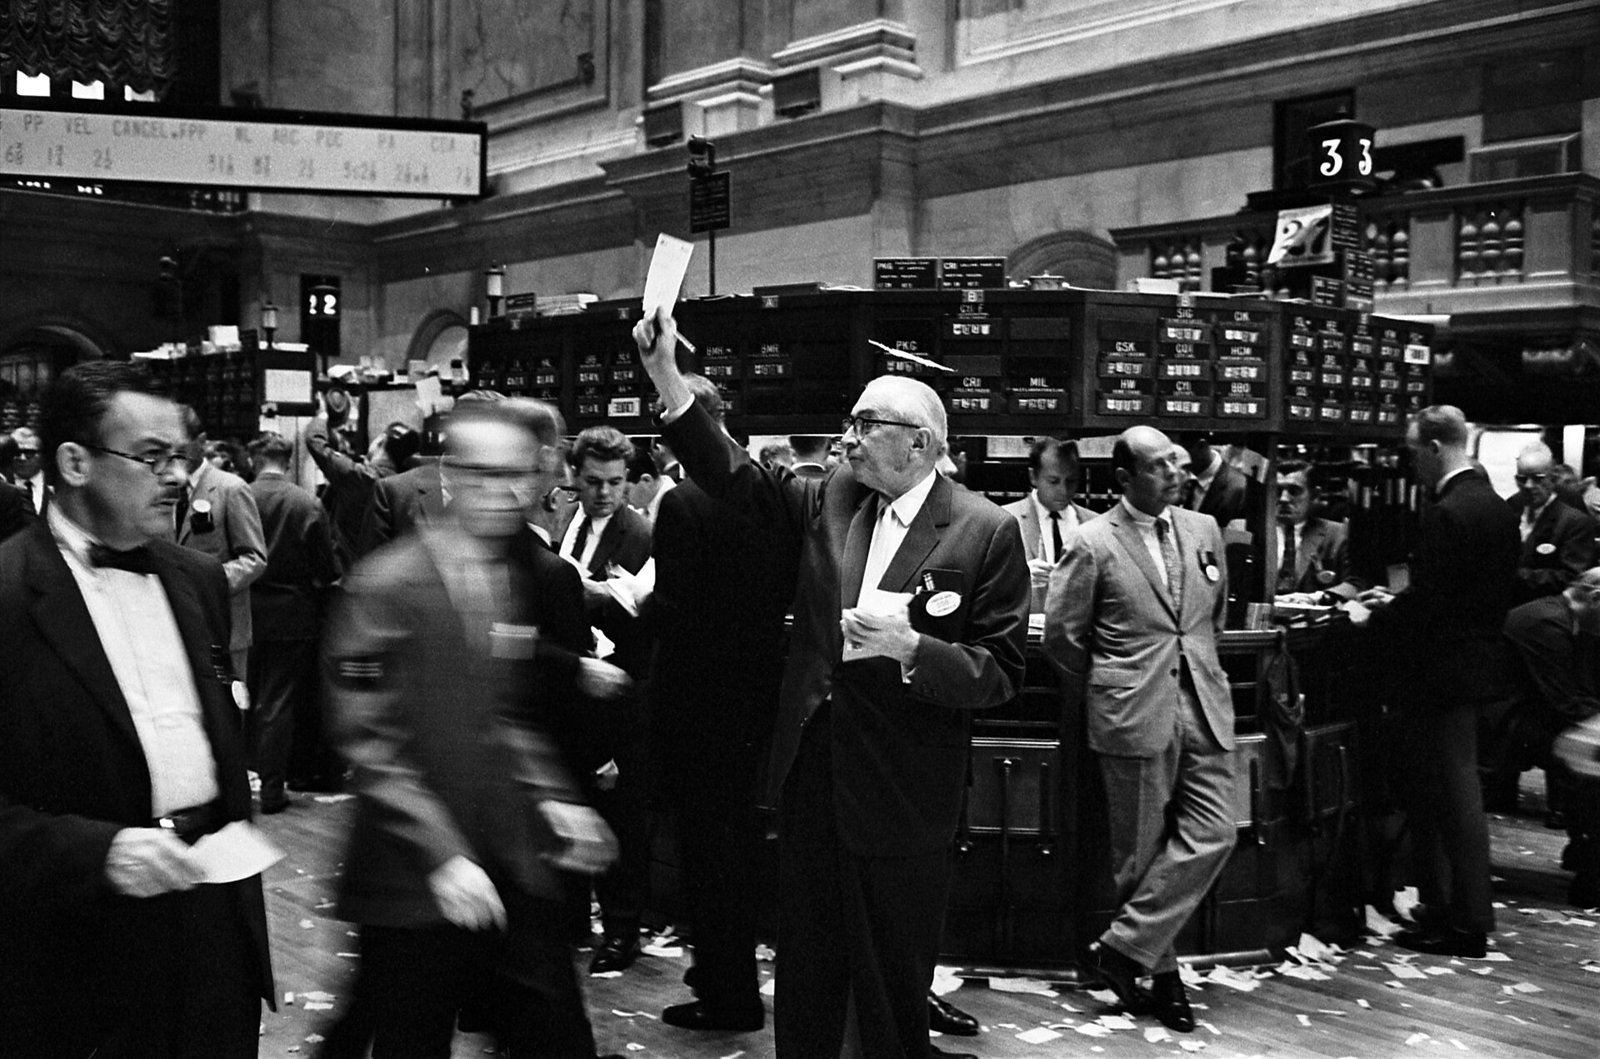
\includegraphics[height=0.36\textheight]{ch0_nyse_floor_1963.jpg}\\[1mm]
\imgcap{Ringul de tranzacționare al Bursei din New York, 1963}
\imgcredit{https://commons.wikimedia.org/wiki/File:NY_stock_exchange_traders_floor_LC-U9-10548-6.jpg}{Foto: Thomas J. O'Halloran (1963), Library of Congress; domeniu public; Wikimedia Commons}
\end{column}
\end{columns}
\end{frame}

\begin{frame}{1900: prețurile ca mers aleator}
\itemsize{\small}
\begin{columns}[T]
\begin{column}{0.64\textwidth}
\begin{itemize}
    \item Louis Bachelier, \textit{Théorie de la spéculation} \refBachelier
    \begin{itemize}
        \item primul model matematic al prețurilor: variația unui preț este o sumă de multe șocuri mici aleatoare
        \item cîștigul așteptat al speculatorului este zero
    \end{itemize}
    \item \refKendall: 22 de serii de prețuri britanice se comportă ca o serie „rătăcitoare”
    \begin{itemize}
        \item variațiile de la o săptămînă la alta seamănă cu extrageri independente
    \end{itemize}
    \item \refRoberts: mersurile aleatoare simulate arată „tipare” pe care analiștii tehnici le văd în prețurile reale
\end{itemize}
\end{column}
\begin{column}{0.32\textwidth}
\centering

\includegraphics[height=0.42\textheight]{ch0_bachelier.jpg}\\[1mm]
\imgcap{Louis Bachelier (1870--1946)}
\imgcredit{https://commons.wikimedia.org/wiki/File:LouisBachelier.jpg}{Foto: autor necunoscut; domeniu public; Wikimedia Commons}
\end{column}
\end{columns}
\end{frame}

\begin{frame}{Care este S\&P 500?}
\itemsize{\footnotesize}
\begin{center}
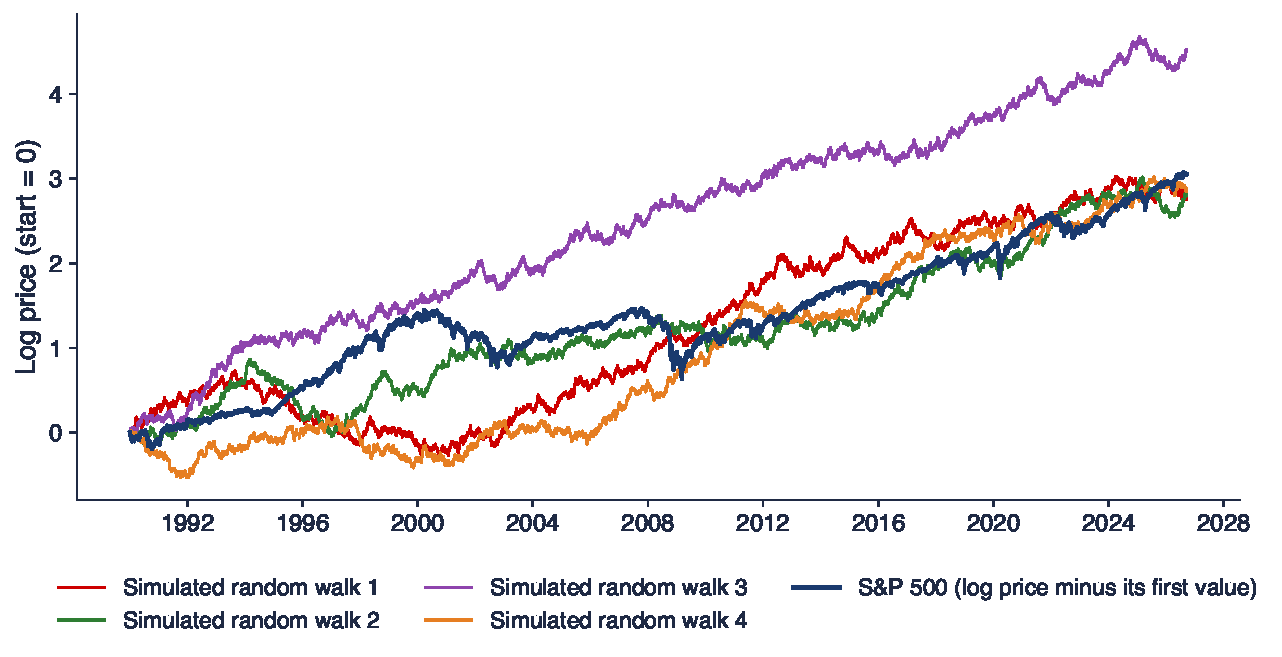
\includegraphics[width=0.97\textwidth,height=0.56\textheight,keepaspectratio]{sfm_ch7_rw_paths.pdf}
\end{center}
\vspace{-0.25cm}
\begin{itemize}
    \item Patru mersuri aleatoare cu pași Normali i.i.d.\ (media $0{,}033\%$, abaterea standard $1{,}13\%$ pe zi, ca la S\&P 500) și prețul logaritmic S\&P 500 din 1990
    \item \textbf{Întrebare pentru sală}: fără legendă, ați putea spune care traiectorie este cea reală?
    \item \textbf{Răspuns}: greu; avînturile și căderile lungi apar și în zgomotul pur (valori finale: $2{,}76$--$4{,}50$; S\&P 500: $3{,}06$)
\end{itemize}
\sfmquantlet{Ch_07}{SFM_ch7_random_walk}
\end{frame}

\begin{frame}{1965: prețurile anticipate corect fluctuează aleator}
\itemsize{\small}
\begin{columns}[T]
\begin{column}{0.54\textwidth}
\begin{itemize}
    \item Paul Samuelson \refSamuelson: dacă prețurile conțin deja tot ce anticipează investitorii, următoarea variație este imprevizibilă
    \begin{itemize}
        \item formal: prețul este un \textbf{martingal}, $E[P_{t+1} \mid \mathcal{F}_t] = P_t$ (\sfmchlink{https://danpele.github.io/SFM/RO/Cursuri/capitol4_probabilitate.pdf}{Capitolul 4})
        \item $\mathcal{F}_t$: informația disponibilă la momentul $t$
    \end{itemize}
    \item Caracterul aleator al variațiilor de preț este semnul unei piețe care funcționează, nu al haosului
    \item \refFamaC: randamentele zilnice ale celor 30 de acțiuni Dow Jones nu arată aproape deloc autocorelație
\end{itemize}
\end{column}
\begin{column}{0.42\textwidth}
\centering
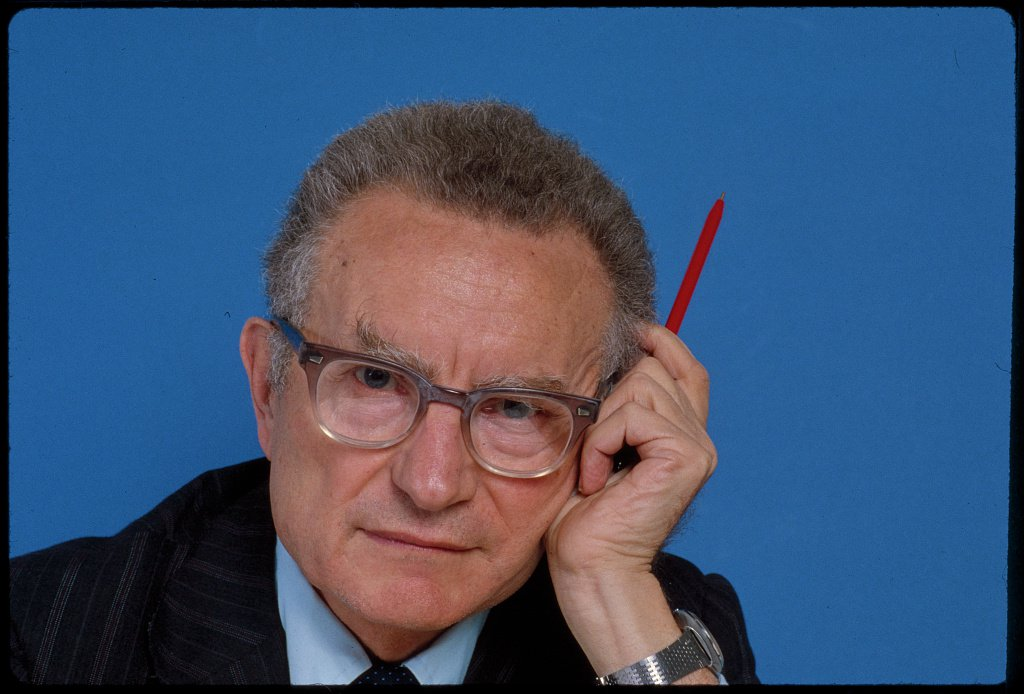
\includegraphics[height=0.34\textheight]{ch7_samuelson.jpg}\\[1mm]
\imgcap{Paul A. Samuelson (1915--2009), Premiul Nobel 1970}
\imgcredit{https://commons.wikimedia.org/wiki/File:Paul_A._Samuelson,_economist.jpg}{Foto: Bernard Gotfryd (1970--1975); domeniu public; Wikimedia Commons}
\end{column}
\end{columns}
\end{frame}

\begin{frame}{Ne spune randamentul de ieri ceva despre cel de azi?}
\itemsize{\footnotesize}
\begin{center}
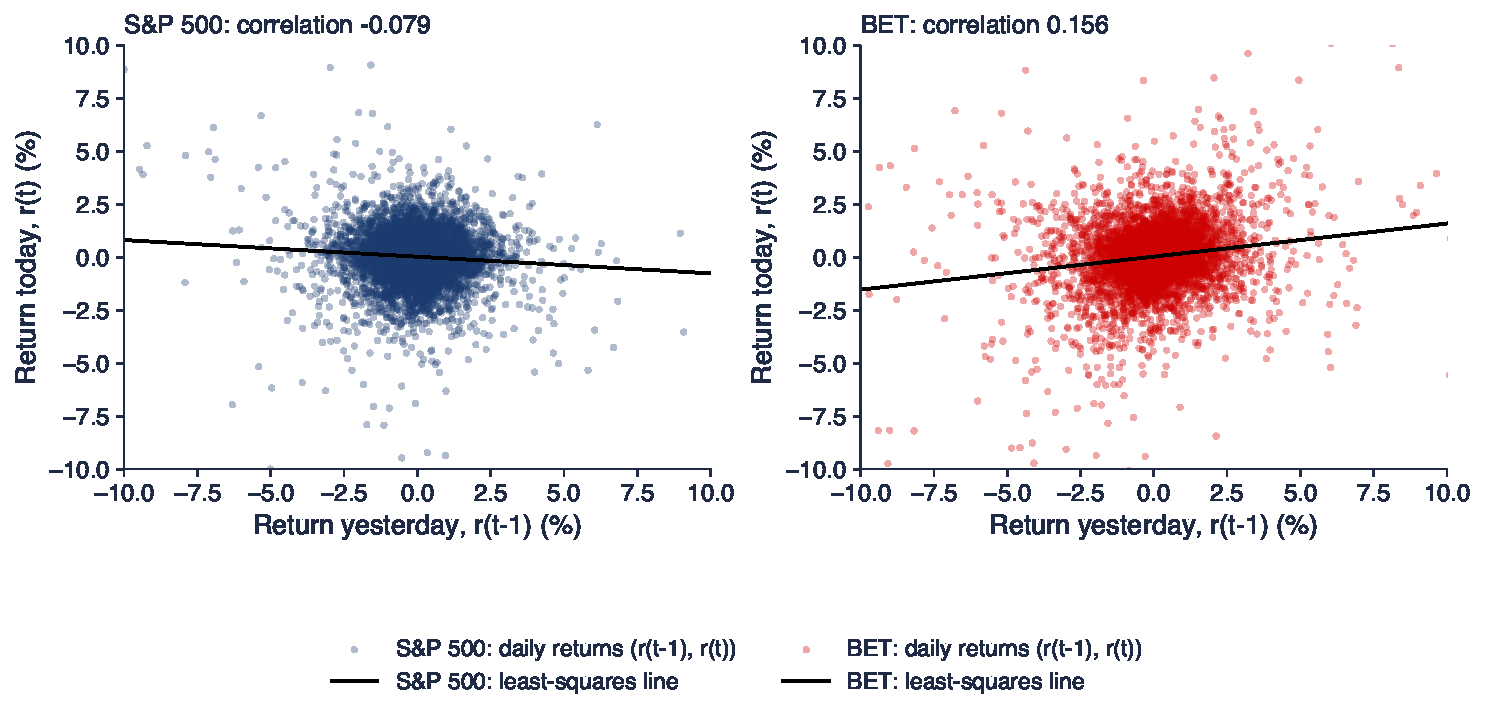
\includegraphics[width=0.97\textwidth,height=0.58\textheight,keepaspectratio]{sfm_ch7_scatter_lag.pdf}
\end{center}
\vspace{-0.25cm}
\begin{itemize}
    \item Fiecare punct: (randamentul de ieri, randamentul de azi); dreapta: cele mai mici pătrate; panta ei este prima autocorelație $\hat\rho(1)$
    \item S\&P 500: $\hat\rho(1) = -0{,}079$ (o ușoară revenire); BET: $\hat\rho(1) = 0{,}156$ (o ușoară continuare); sînt aceste valori diferite de zero?
\end{itemize}
\sfmquantlet{Ch_07}{SFM_ch7_random_walk}
\end{frame}

\begin{frame}{Recapitulare: pot fi anticipate prețurile?}
\itemsize{\small}
\begin{itemize}
    \item De la Bachelier (1900) la Samuelson (1965): variațiile prețurilor par aleatoare, iar economia explică de ce
    \item Investitorii profesioniști bat rar piața după costuri
    \item Autocorelațiile zilnice sînt mici, dar nu nule: avem nevoie de teste, nu de impresii
\end{itemize}
\end{frame}


%=============================================================================
\section{Piețe eficiente}
%=============================================================================

\begin{frame}{Ce este o piață eficientă?}
\itemsize{\small}
\begin{columns}[T]
\begin{column}{0.60\textwidth}
\begin{itemize}
    \item \textbf{EMH} (efficient market hypothesis, ipoteza pieței eficiente) \refFamaA: prețurile „reflectă pe deplin” informația disponibilă $\Omega_t$
    \begin{itemize}
        \item nicio regulă de tranzacționare care folosește $\Omega_t$ nu cîștigă mai mult decît randamentul care îi compensează riscul
        \item prețurile se mișcă doar la \textbf{știri}: informație care nu era în $\Omega_t$
    \end{itemize}
    \item Eficiența este relativă la o mulțime de informații
    \begin{itemize}
        \item cu cît $\Omega_t$ este mai mică, cu atît afirmația este mai slabă și testul mai ușor
    \end{itemize}
    \item Eficient nu înseamnă „randamente zero”: randamentul așteptat remunerează riscul
\end{itemize}
\end{column}
\begin{column}{0.36\textwidth}
\centering

\includegraphics[height=0.42\textheight]{ch0_fama_2013.jpg}\\[1mm]
\imgcap{Eugene F. Fama, Premiul Nobel 2013}
\imgcredit{https://commons.wikimedia.org/wiki/File:Eugene_Fama_at_Nobel_Prize,_2013.jpg}{Foto: Bengt Nyman (2013); CC BY 2.0; Wikimedia Commons}
\end{column}
\end{columns}
\end{frame}

\begin{frame}{Trei forme ale eficienței}
\itemsize{\small}
\begin{center}
\footnotesize
\begin{tabular}{>{\raggedright\arraybackslash}p{1.8cm}>{\raggedright\arraybackslash}p{3.2cm}>{\raggedright\arraybackslash}p{3.0cm}>{\raggedright\arraybackslash}p{2.9cm}}
\toprule
\textbf{Forma} & \textbf{Mulțimea de informații $\Omega_t$} & \textbf{Ce nu poate aduce randamente în exces} & \textbf{Testul tipic} \\
\midrule
Slabă & prețurile și randamentele trecute & analiza tehnică, tiparele grafice & autocorelație, runs, variance ratio \\
Semi-tare & toată informația publică & analiza fundamentală a datelor publice & studii de eveniment \\
Tare & toată informația, inclusiv cea privată & informația privilegiată & randamentele insiderilor și ale administratorilor de fonduri \\
\bottomrule
\end{tabular}
\end{center}
\begin{itemize}
    \item Formele sînt incluse una în alta: tare $\Rightarrow$ semi-tare $\Rightarrow$ slabă; respingerea formei slabe le respinge pe toate trei
    \item Acest capitol testează mai ales forma slabă: prețurile trecute sînt date gratuite pentru oricine \refFamaA, \refFamaB
\end{itemize}
\end{frame}

\begin{frame}{Modelul jocului echitabil}
\itemsize{\small}
\begin{itemize}
    \item Fie $r_{t+1}$ randamentul unui activ și $E[r_{t+1} \mid \Omega_t]$ \textbf{randamentul așteptat de echilibru} (randamentul care îi remunerează riscul)
    \begin{itemize}
        \item \textbf{randamentul în exces} (surpriza): $z_{t+1} = r_{t+1} - E[r_{t+1} \mid \Omega_t]$
    \end{itemize}
    \item \textbf{Joc echitabil}: $E[z_{t+1} \mid \Omega_t] = 0$
    \begin{itemize}
        \item erorile de prognoză sînt nule în medie, orice am ști la momentul $t$
        \item o regulă care investește $w(\Omega_t)$ cîștigă $E[w(\Omega_t)\, z_{t+1}] = 0$ peste echilibru
    \end{itemize}
    \item Cu un randament așteptat constant $\mu$: $E[r_{t+1} \mid \Omega_t] = \mu$; randamentele minus $\mu$ sînt o \textbf{diferență de martingal}
    \item Definiția nu cere nici varianță constantă, nici distribuția Normală
\end{itemize}
\end{frame}

\begin{frame}{Problema ipotezei comune}
\itemsize{\small}
\begin{itemize}
    \item Pentru a testa eficiența trebuie să știm randamentul așteptat de echilibru $E[r_{t+1} \mid \Omega_t]$
    \begin{itemize}
        \item pentru asta ne trebuie un model de echilibru: medie constantă, CAPM (capital asset pricing model, modelul de evaluare a activelor financiare), modele cu factori
    \end{itemize}
    \item Orice test al eficienței este un \textbf{test comun} al eficienței și al modelului \refFamaB
    \begin{itemize}
        \item o respingere poate însemna o piață ineficientă sau un model greșit al randamentelor așteptate
        \item eficiența, luată separat, nu poate fi respinsă niciodată
    \end{itemize}
    \item Pentru randamentele zilnice problema contează puțin: randamentele așteptate zilnice sînt foarte mici (circa $0{,}033\%$ pentru S\&P 500), deci orice model rezonabil dă aproape același răspuns
\end{itemize}
\end{frame}

\begin{frame}{Paradoxul Grossman--Stiglitz}
\itemsize{\small}
\begin{itemize}
    \item Informația costă: trebuie colectată și analizată \refGS
    \begin{itemize}
        \item dacă prețurile ar reflecta perfect toată informația, nimeni nu ar fi plătit pentru a o colecta
        \item atunci nimeni nu ar mai colecta-o, iar prețurile nu ar mai putea s-o reflecte
    \end{itemize}
    \item Concluzie: o piață poate fi doar \textbf{aproape} eficientă
    \begin{itemize}
        \item micile ineficiențe acoperă costurile investitorilor informați
        \item întrebarea devine „cît de eficientă, unde și cînd?”, nu „da sau nu?”
    \end{itemize}
    \item Această perspectivă duce la ipoteza piețelor adaptive din secțiunea 8
\end{itemize}
\end{frame}

\begin{frame}{2013: un Premiu Nobel, două perspective}
\itemsize{\footnotesize}
\begin{columns}[T]
\begin{column}{0.48\textwidth}
\centering

\includegraphics[height=0.38\textheight]{ch0_fama_2013.jpg}\\[1mm]
\imgcap{Eugene F. Fama: prețurile sînt greu de anticipat pe zile și săptămîni}
\imgcredit{https://commons.wikimedia.org/wiki/File:Eugene_Fama_at_Nobel_Prize,_2013.jpg}{Foto: Bengt Nyman (2013); CC BY 2.0; Wikimedia Commons}
\end{column}
\begin{column}{0.48\textwidth}
\centering

\includegraphics[height=0.38\textheight]{ch7_shiller_2013.jpg}\\[1mm]
\imgcap{Robert J. Shiller: prețurile oscilează prea mult față de valorile fundamentale}
\imgcredit{https://commons.wikimedia.org/wiki/File:Robert_J._Shiller_(50372668186).jpg}{Foto: Bengt Nyman (2013); CC BY 2.0; Wikimedia Commons}
\end{column}
\end{columns}\begin{itemize}
    \item Amîndoi au dreptate, pe orizonturi diferite: randamentele pe termen scurt sînt aproape imprevizibile; cele pe termen lung sînt parțial previzibile din indicatorii de evaluare
\end{itemize}
\end{frame}

\begin{frame}{Recapitulare: piețe eficiente}
\itemsize{\small}
\begin{itemize}
    \item Eficiența se definește relativ la o mulțime de informații: slabă, semi-tare, tare
    \item Joc echitabil: randamentele în exces sînt imprevizibile, condiționat de $\Omega_t$
    \item Orice test este un test comun cu un model al randamentelor așteptate
    \item Informația costisitoare face imposibilă eficiența perfectă \refGS
\end{itemize}
\end{frame}


%=============================================================================
\section{Ipotezele mersului aleator}
%=============================================================================

\begin{frame}{Modelul mersului aleator pentru prețurile logaritmice}
\itemsize{\small}
\begin{itemize}
    \item Prețul logaritmic $p_t = \ln P_t$; \textbf{mers aleator cu tendință (drift)} $\mu$: $p_t = \mu + p_{t-1} + \varepsilon_t$
    \begin{itemize}
        \item randamentul $r_t = p_t - p_{t-1} = \mu + \varepsilon_t$: creșterile $\varepsilon_t$ au media 0
        \item prin recurență: $p_t = p_0 + \mu t + \sum_{s=1}^{t} \varepsilon_s$: fiecare șoc este \textbf{permanent}
    \end{itemize}
    \item Dacă $\varepsilon_t$ sînt necorelate, cu varianța $\sigma^2$:
    \begin{itemize}
        \item $E[p_t] = p_0 + \mu t$ și $\mathrm{Var}(p_t - p_0) = t\sigma^2$: incertitudinea crește cu orizontul
        \item randamentul pe $q$ zile $r_t(q) = r_t + \dots + r_{t-q+1}$ are $\mathrm{Var}(r_t(q)) = q\sigma^2$
    \end{itemize}
    \item Prețuri logaritmice, nu prețuri: $P_t$ nu poate deveni negativ, iar randamentele logaritmice se adună în timp (\sfmchlink{https://danpele.github.io/SFM/RO/Cursuri/capitol1_date_randamente_indicatori.pdf}{Capitolul 1})
\end{itemize}
\end{frame}

\begin{frame}{Trei ipoteze de mers aleator}
\itemsize{\small}
\begin{itemize}
    \item \textbf{RW1} (creșteri i.i.d.): $\varepsilon_t$ independente și identic distribuite, $\varepsilon_t \sim \mathrm{IID}(0, \sigma^2)$ \refCLM
    \begin{itemize}
        \item cea mai puternică: nicio funcție a trecutului nu anticipează vreo funcție a viitorului
    \end{itemize}
    \item \textbf{RW2} (creșteri independente): $\varepsilon_t$ independente, dar nu identic distribuite
    \begin{itemize}
        \item permite varianței să se schimbe în timp într-un mod care nu poate fi anticipat din trecut (regimuri)
    \end{itemize}
    \item \textbf{RW3} (creșteri necorelate): $\mathrm{Cov}(\varepsilon_t, \varepsilon_{t-k}) = 0$ pentru orice $k \ne 0$
    \begin{itemize}
        \item cea mai slabă: permite $\mathrm{Cov}(\varepsilon_t^2, \varepsilon_{t-k}^2) \ne 0$, adică volatility clustering
    \end{itemize}
    \item Incluse una în alta: RW1 $\Rightarrow$ RW2 $\Rightarrow$ RW3; testele RW3 folosesc doar autocorelațiile randamentelor
\end{itemize}
\end{frame}

\begin{frame}{Comparația ipotezelor de mers aleator}
\itemsize{\small}
\begin{center}
\footnotesize
\begin{tabular}{lcccc}
\toprule
\textbf{Proprietatea randamentelor} & RW1 & RW2 & RW3 & \textbf{Martingal} \\
\midrule
$\mathrm{Corr}(r_t, r_{t-k}) = 0$ & da & da & da & da \\
$E[r_t \mid \text{trecut}] = \mu$ (media imprevizibilă) & da & da & nu mereu & da \\
varianță constantă & da & nu & nu & nu \\
admite volatility clustering & nu & nu & da & da \\
randamentele GARCH (Capitolul 9) o satisfac & nu & nu & da & da \\
\bottomrule
\end{tabular}
\end{center}
\begin{itemize}
    \item \textbf{GARCH} (generalised autoregressive conditional heteroskedasticity, heteroscedasticitate condiționată autoregresivă generalizată): varianța de mîine depinde de șocurile de azi; media rămîne imprevizibilă
    \item Eficiența în formă slabă cere doar un martingal (sau RW3), nu RW1
\end{itemize}
\end{frame}

\begin{frame}{Martingal și mers aleator}
\itemsize{\small}
\begin{itemize}
    \item $\{p_t - \mu t\}$ este un \textbf{martingal} dacă $E[p_{t+1} - \mu(t+1) \mid \mathcal{F}_t] = p_t - \mu t$ \refSamuelson
    \begin{itemize}
        \item echivalent, $E[r_{t+1} - \mu \mid \mathcal{F}_t] = 0$: randamentele minus $\mu$ sînt o diferență de martingal
        \item o diferență de martingal cu varianță finită este necorelată: martingal $\Rightarrow$ RW3
    \end{itemize}
    \item RW1 și RW2 implică martingalul; reciproca nu este adevărată: un martingal poate avea varianța previzibilă
    \item \textbf{Întrebare pentru sală}: este volatility clustering în contradicție cu eficiența în formă slabă?
    \begin{itemize}
        \item \textbf{Răspuns}: nu; respinge RW1 și RW2, dar o varianță previzibilă nu face randamentul previzibil; martingalul și RW3 rămîn valabile
    \end{itemize}
\end{itemize}
\end{frame}

\begin{frame}{Exemplu lucrat: cum crește riscul cu orizontul}
\itemsize{\small}
\begin{itemize}
    \item S\&P 500 din 1990: abaterea standard zilnică $\hat\sigma = 1{,}13\%$
    \begin{itemize}
        \item în ipoteza de mers aleator, $\mathrm{sd}(r_t(q)) = \sigma\sqrt{q}$
    \end{itemize}
    \item Pas cu pas
    \begin{itemize}
        \item o săptămînă, $q = 5$: $1{,}13 \times \sqrt{5} = 1{,}13 \times 2{,}24 = 2{,}53\%$
        \item o lună, $q = 20$: $1{,}13 \times 4{,}47 = 5{,}07\%$
        \item un an, $q = 250$: $1{,}13 \times 15{,}81 = 17{,}92\%$
    \end{itemize}
    \item Aceasta este „regula rădăcinii pătrate a timpului”, folosită pentru a scala VaR și volatilitatea
    \item Dacă randamentele sînt autocorelate, regula nu mai funcționează: testul variance ratio din secțiunea 7 măsoară cu cît
\end{itemize}
\end{frame}

\begin{frame}{Recapitulare: ipotezele mersului aleator}
\itemsize{\small}
\begin{itemize}
    \item $p_t = \mu + p_{t-1} + \varepsilon_t$: șocuri permanente, $\mathrm{Var}(r_t(q)) = q\sigma^2$
    \item RW1 (i.i.d.) $\Rightarrow$ RW2 (independente) $\Rightarrow$ RW3 (necorelate)
    \item Martingal: media imprevizibilă, varianța posibil previzibilă; ipoteza nulă potrivită pentru eficiență
\end{itemize}
\end{frame}


%=============================================================================
\section{Zgomotul alb și funcția de autocorelație}
%=============================================================================

\begin{frame}{Zgomot alb și autocorelație}
\itemsize{\small}
\begin{itemize}
    \item \textbf{Autocovarianța} la decalajul $k$: $\gamma(k) = \mathrm{Cov}(x_t, x_{t-k})$; \textbf{autocorelația}: $\rho(k) = \gamma(k)/\gamma(0)$
    \begin{itemize}
        \item \textbf{ACF} (autocorrelation function, funcția de autocorelație): $k \mapsto \rho(k)$, $k = 1, 2, \dots$
    \end{itemize}
    \item \textbf{Zgomot alb}: media 0, varianța constantă $\sigma^2$, $\rho(k) = 0$ pentru orice $k \ne 0$
    \begin{itemize}
        \item zgomotul i.i.d.\ este zgomot alb; zgomotul alb gaussian este i.i.d.\ $N(0, \sigma^2)$
        \item zgomotul alb nu trebuie să fie independent: randamentele GARCH sînt zgomot alb, dar nu i.i.d.
    \end{itemize}
    \item \textbf{ACF de selecție}: $\hat\rho(k) = \sum_{t=k+1}^{T}(x_t - \bar x)(x_{t-k} - \bar x)\big/\sum_{t=1}^{T}(x_t - \bar x)^2$
    \begin{itemize}
        \item pentru date i.i.d., $\hat\rho(k) \approx N(0, 1/T)$: banda de 95\% $\pm 1{,}96/\sqrt{T}$
    \end{itemize}
\end{itemize}
\end{frame}

\begin{frame}{Zgomotul alb gaussian și ACF-ul lui de selecție}
\itemsize{\footnotesize}
\begin{center}
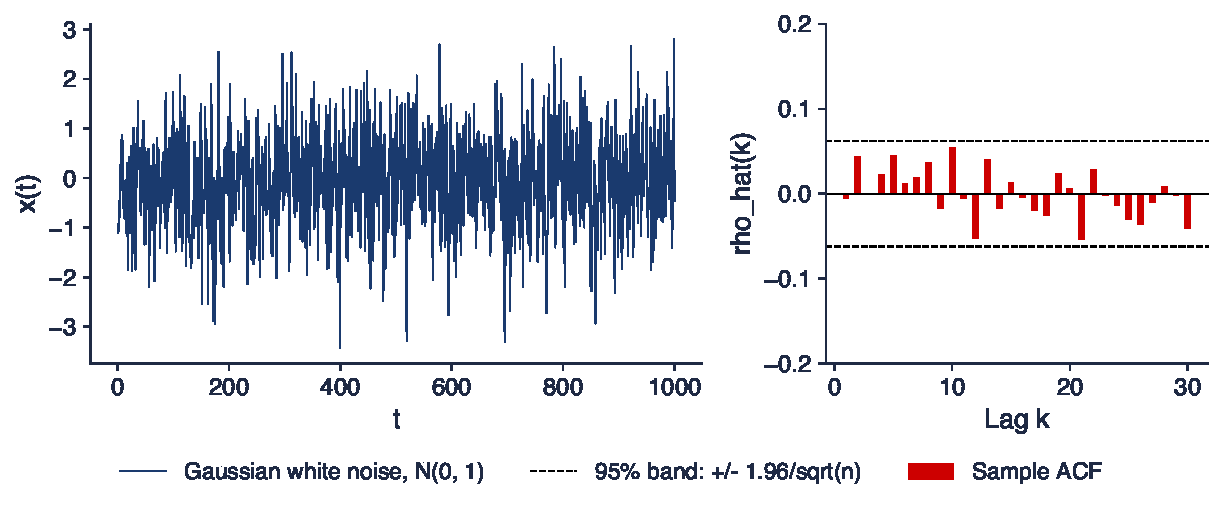
\includegraphics[width=0.97\textwidth,height=0.56\textheight,keepaspectratio]{sfm_ch7_white_noise.pdf}
\end{center}
\vspace{-0.25cm}
\begin{itemize}
    \item Stînga: 1\,000 de extrageri din $N(0, 1)$ (ca în SFEtimewn); dreapta: $\hat\rho(1), \dots, \hat\rho(30)$ cu banda $\pm 1{,}96/\sqrt{1000} = \pm 0{,}062$
    \item Aici 0 din 30 de autocorelații ies din bandă; cu 30 de decalaje ne așteptăm la circa 1,5 doar din întîmplare
\end{itemize}
\sfmquantlet{Ch_07}{SFM_ch7_white_noise_acf}
\end{frame}

\begin{frame}{ACF-ul proceselor AR și MA}
\itemsize{\small}
\begin{itemize}
    \item \textbf{AR(1)} (autoregresiv): $x_t = \alpha x_{t-1} + \varepsilon_t$, $|\alpha| < 1$: $\rho(k) = \alpha^k$
    \begin{itemize}
        \item scădere geometrică; semne alternante dacă $\alpha < 0$; exemplu: $\alpha = 0{,}9 \Rightarrow \rho(3) = 0{,}9^3 = 0{,}729$
    \end{itemize}
    \item \textbf{AR(2)}: $x_t = \alpha_1 x_{t-1} + \alpha_2 x_{t-2} + \varepsilon_t$: $\rho(1) = \alpha_1/(1 - \alpha_2)$, $\rho(k) = \alpha_1\rho(k-1) + \alpha_2\rho(k-2)$
    \begin{itemize}
        \item $\alpha_1 = 0{,}5$, $\alpha_2 = 0{,}4$: $\rho(1) = 0{,}5/0{,}6 = 0{,}833$, $\rho(2) = 0{,}5 \times 0{,}833 + 0{,}4 = 0{,}817$
    \end{itemize}
    \item \textbf{MA(1)} (moving average, medie mobilă): $x_t = \varepsilon_t + \beta\varepsilon_{t-1}$: $\rho(1) = \beta/(1 + \beta^2)$, $\rho(k) = 0$ pentru $k \ge 2$
    \begin{itemize}
        \item $\beta = 0{,}5$: $\rho(1) = 0{,}5/1{,}25 = 0{,}40$; un MA($q$) are un ACF care se anulează după decalajul $q$
    \end{itemize}
    \item Forma ACF-ului arată tipul de dependență: scădere lentă (AR), anulare bruscă (MA), nimic (zgomot alb)
\end{itemize}
\end{frame}

\begin{frame}{ACF-ul teoretic și de selecție pentru șase procese}
\itemsize{\footnotesize}
\begin{center}
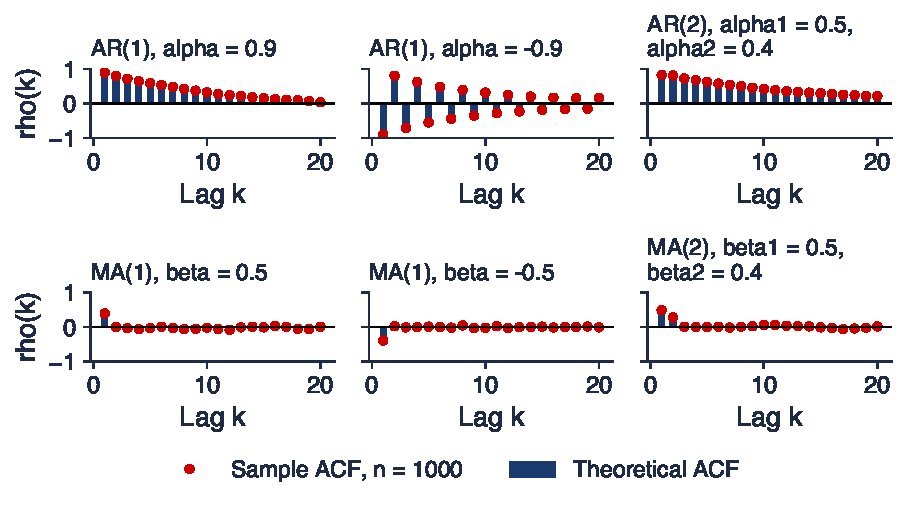
\includegraphics[width=0.97\textwidth,height=0.60\textheight,keepaspectratio]{sfm_ch7_acf_processes.pdf}
\end{center}
\vspace{-0.25cm}
\begin{itemize}
    \item Bare: $\rho(k)$ teoretic; puncte: ACF-ul de selecție al unei traiectorii simulate de 1\,000 de valori (SFEacfar1, SFEacfar2, SFEacfma1, SFEacfma2)
    \item Un mers aleator este limita $\alpha \to 1$ a AR(1): ACF-ul lui nu ar scădea deloc
\end{itemize}
\sfmquantlet{Ch_07}{SFM_ch7_white_noise_acf}
\end{frame}

\begin{frame}{ACF-ul randamentelor zilnice}
\itemsize{\footnotesize}
\begin{center}
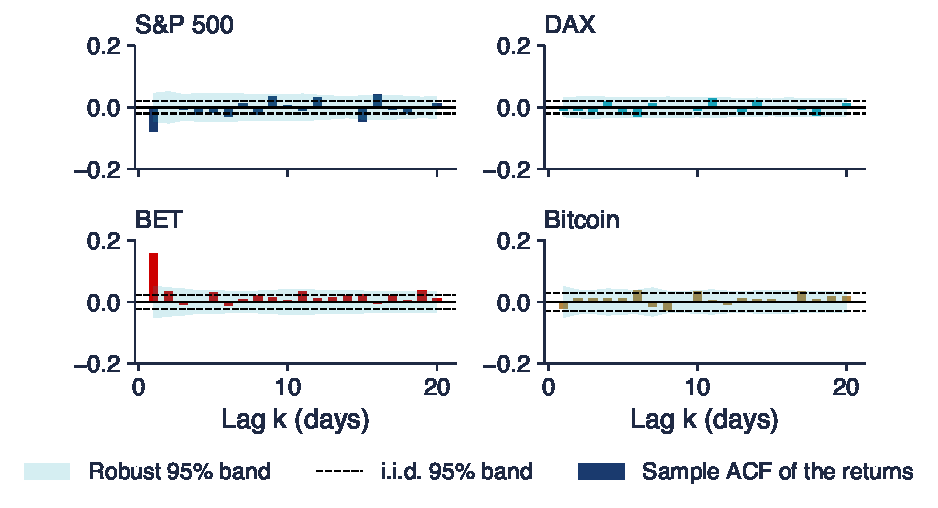
\includegraphics[width=0.97\textwidth,height=0.62\textheight,keepaspectratio]{sfm_ch7_acf_returns.pdf}
\end{center}
\vspace{-0.25cm}
\begin{itemize}
    \item Bare: $\hat\rho(1), \dots, \hat\rho(20)$; linia întreruptă: banda i.i.d.\ $\pm 1{,}96/\sqrt{T}$; zona umbrită: banda robustă (slide-ul următor)
\end{itemize}
\sfmquantlet{Ch_07}{SFM_ch7_autocorrelation_tests}
\end{frame}

\begin{frame}{Interpretarea ACF-ului randamentelor}
\itemsize{\small}
\begin{itemize}
    \item Primele autocorelații: S\&P 500 $-0{,}079$, DAX $-0{,}009$, BET $0{,}156$, Bitcoin $-0{,}022$
    \begin{itemize}
        \item doar S\&P 500 și BET ies în evidență la decalajul 1, cu semne opuse
    \end{itemize}
    \item Banda \textbf{robustă}: $\pm 1{,}96\sqrt{\hat\delta(k)/T}$, $\hat\delta(k) = T\sum_t e_t^2 e_{t-k}^2/(\sum_t e_t^2)^2$, $e_t = r_t - \bar r$ \refLM
    \begin{itemize}
        \item randamente i.i.d.: $\hat\delta(k) \approx 1$; volatility clustering: randamentele mari în modul urmează după randamente mari în modul, deci $\hat\delta(k) > 1$
        \item S\&P 500 la decalajul 1: $\pm 0{,}046$ în loc de $\pm 0{,}020$
    \end{itemize}
    \item S\&P 500, numărul de decalaje (din 20) aflate în afara benzii: 9 cu banda i.i.d., 3 cu banda robustă
    \item Banda i.i.d.\ testează RW1; banda robustă testează RW3, ipoteza care contează pentru eficiență
\end{itemize}\sfmquantlet{Ch_07}{SFM_ch7_autocorrelation_tests}
\end{frame}

\begin{frame}{Randamentele sînt aproape necorelate, mărimea lor nu}
\itemsize{\footnotesize}
\begin{center}
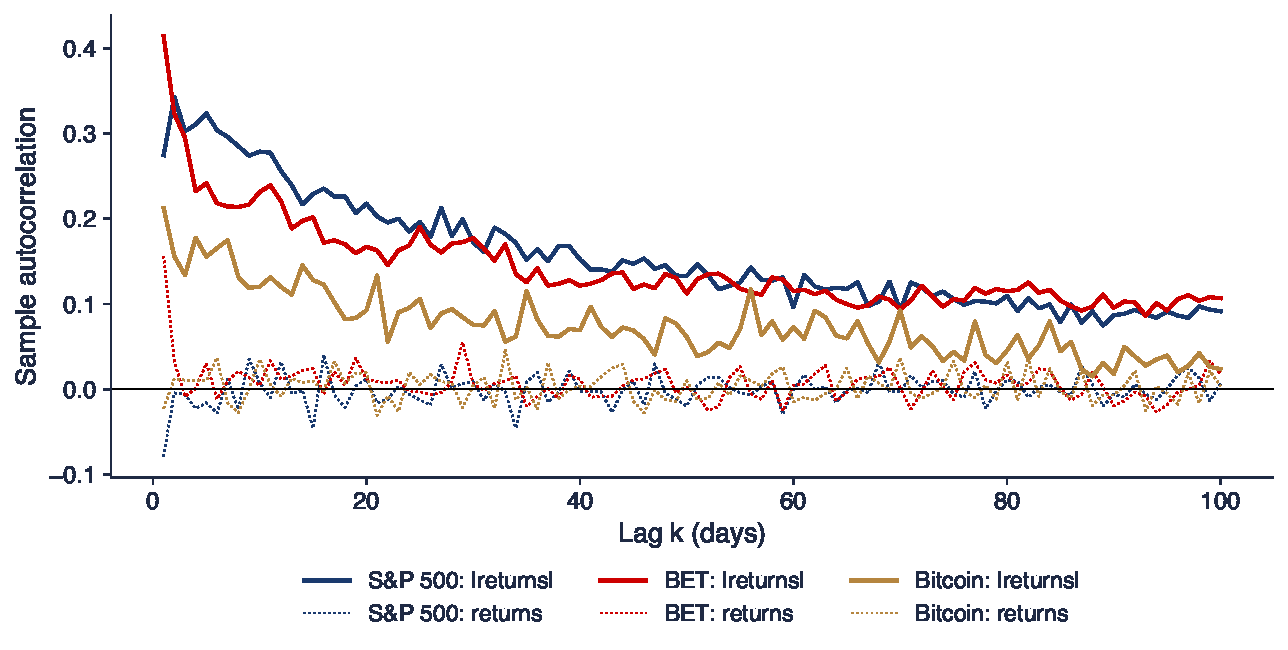
\includegraphics[width=0.97\textwidth,height=0.56\textheight,keepaspectratio]{sfm_ch7_acf_abs.pdf}
\end{center}
\vspace{-0.25cm}
\begin{itemize}
    \item ACF-ul lui $|r_t|$: S\&P 500 $0{,}27$ la decalajul 1, $0{,}22$ la decalajul 20, $0{,}09$ la decalajul 100; randamentele însele: linii punctate în jurul lui 0
    \item Mișcările mari urmează după mișcări mari: RW1 și RW2 sînt respinse la prima vedere; graficul nu spune nimic despre RW3 și martingal
\end{itemize}
\sfmquantlet{Ch_07}{SFM_ch7_autocorrelation_tests}
\end{frame}

\begin{frame}{Recapitulare: zgomotul alb și ACF}
\itemsize{\small}
\begin{itemize}
    \item Zgomot alb: necorelat; zgomot i.i.d.: independent; randamentele GARCH: zgomot alb, nu i.i.d.
    \item AR: scădere geometrică a ACF; MA($q$): anulare după $q$ decalaje
    \item Folosiți banda robustă $\pm 1{,}96\sqrt{\hat\delta(k)/T}$ pentru randamente: banda i.i.d.\ este prea îngustă
\end{itemize}
\end{frame}


%=============================================================================
\section{Testarea autocorelației}
%=============================================================================

\begin{frame}{Teste portmanteau: Box--Pierce și Ljung--Box}
\itemsize{\small}
\begin{itemize}
    \item $H_0$: $\rho(1) = \dots = \rho(m) = 0$; $H_1$: cel puțin un $\rho(k) \ne 0$; un singur test pentru $m$ decalaje împreună
    \begin{itemize}
        \item „portmanteau”: un geamantan în care încap multe autocorelații deodată
    \end{itemize}
    \item Box--Pierce \refBP: $Q_{BP}(m) = T\sum_{k=1}^{m} \hat\rho(k)^2$
    \item \textbf{LB} (Ljung--Box) \refLjung: $Q_{LB}(m) = T(T+2)\sum_{k=1}^{m} \dfrac{\hat\rho(k)^2}{T - k}$, mai aproape de $\chi^2$ în eșantioane mici
    \begin{itemize}
        \item pentru randamente i.i.d.\ ambele $\sim \chi^2(m)$; respingem $H_0$ dacă $Q > \chi^2_{0{,}95}(m)$; $\chi^2_{0{,}95}(10) = 18{,}31$
    \end{itemize}
    \item Alegerea lui $m$: aici $m = 10$ (două săptămîni de tranzacționare); un $m$ mai mare diluează un efect de scurtă durată
\end{itemize}
\end{frame}

\begin{frame}{Exemplu lucrat: Ljung--Box pas cu pas}
\itemsize{\small}
\begin{itemize}
    \item $T = 1000$ de randamente zilnice, $\hat\rho(1) = 0{,}06$, $\hat\rho(2) = -0{,}04$, $\hat\rho(3) = 0{,}03$; testăm cu $m = 3$
    \begin{itemize}
        \item $T\hat\rho(k)^2$: $3{,}6$; $1{,}6$; $0{,}9$; suma lor: $Q_{BP}(3) = 6{,}10$
        \item $Q_{LB}(3) = 1000 \times 1002 \times (0{,}06^2/999 + 0{,}04^2/998 + 0{,}03^2/997) = 6{,}12$
    \end{itemize}
    \item Decizia: $\chi^2_{0{,}95}(3) = 7{,}81 > 6{,}12$: nu respingem $H_0$ la 5\%
    \begin{itemize}
        \item observație: $\hat\rho(1) = 0{,}06$ se află chiar în interiorul benzii $\pm 1{,}96/\sqrt{1000} = \pm 0{,}062$; nici testul comun nu respinge
    \end{itemize}
    \item Cu aceleași autocorelații și $T = 5000$, $Q$ este de cinci ori mai mare și respingerea este clară: în eșantioanele lungi, autocorelațiile mici devin semnificative
\end{itemize}
\end{frame}

\begin{frame}{Un test portmanteau robust la volatility clustering}
\itemsize{\small}
\begin{itemize}
    \item Distribuția $\chi^2$ a lui $Q_{LB}$ cere $\mathrm{Var}(\hat\rho(k)) = 1/T$: condiție adevărată pentru randamente i.i.d., falsă în prezența volatility clustering
    \begin{itemize}
        \item atunci $Q_{LB}$ respinge un martingal adevărat mult prea des
    \end{itemize}
    \item Statistica \textbf{robustă}: împărțim fiecare $\hat\rho(k)^2$ la propria varianță $\hat\delta(k)/T$ \refEL
    \begin{itemize}
        \item $\tilde Q(m) = \sum_{k=1}^{m} \dfrac{T\hat\rho(k)^2}{\hat\delta(k)} \sim \chi^2(m)$ pentru o diferență de martingal cu momentul de ordin patru finit
        \item cu randamente i.i.d., $\hat\delta(k) \approx 1$ și $\tilde Q \approx Q_{BP}$
    \end{itemize}
    \item Regula: testăm RW1 cu $Q_{LB}$; testăm martingalul (eficiența în formă slabă) cu $\tilde Q$
\end{itemize}
\end{frame}

\begin{frame}{Teste de autocorelație pe date reale}
\itemsize{\footnotesize}
\begin{center}
\scriptsize
\begin{tabular}{lrrrrrrrrr}
\toprule
& $T$ & $\hat\rho(1)$ & $Q_{LB}(10)$ & p & $\tilde Q(10)$ & p & $Q_{LB}(10)$, $r^2$ & runs $z$ & p \\
\midrule
S\&P 500 & 9\,240 & ${-0{,}079}$ & $90{,}8$ & $<$\,0{,}001 & $18{,}8$ & 0{,}043 & $8015$ & ${2{,}97}$ & 0{,}003 \\
DAX & 9\,288 & ${-0{,}009}$ & $21{,}8$ & 0{,}016 & $8{,}6$ & 0{,}571 & $3747$ & ${1{,}73}$ & 0{,}084 \\
BET & 7\,243 & ${0{,}156}$ & $198{,}3$ & $<$\,0{,}001 & $42{,}9$ & $<$\,0{,}001 & $2500$ & ${-7{,}75}$ & $<$\,0{,}001 \\
Bitcoin & 4\,384 & ${-0{,}022}$ & $20{,}2$ & 0{,}028 & $11{,}9$ & 0{,}294 & $213$ & ${2{,}68}$ & 0{,}007 \\
TLV & 3\,788 & ${0{,}010}$ & $29{,}1$ & 0{,}001 & $13{,}2$ & 0{,}210 & $481$ & ${-1{,}68}$ & 0{,}093 \\
SNP & 3\,815 & ${-0{,}015}$ & $20{,}7$ & 0{,}023 & $9{,}9$ & 0{,}446 & $505$ & ${1{,}72}$ & 0{,}085 \\
BRD & 3\,771 & ${0{,}032}$ & $19{,}9$ & 0{,}030 & $10{,}8$ & 0{,}375 & $416$ & ${-3{,}04}$ & 0{,}002 \\
TGN & 3\,725 & ${0{,}055}$ & $28{,}7$ & 0{,}001 & $12{,}3$ & 0{,}263 & $639$ & ${1{,}49}$ & 0{,}136 \\
\bottomrule
\end{tabular}
\end{center}
\begin{itemize}
    \item LB clasic: toate cele opt serii resping la 5\%; $\tilde Q$ robust: doar S\&P 500 (p = 0{,}043) și BET (p = $<$\,0{,}001)
    \item Randamentele la pătrat: $Q_{LB}$ uriaș peste tot: RW1 și RW2 sînt respinse pentru fiecare serie (volatility clustering)
    \item Începutul seriilor: S\&P 500 și DAX 1990; BET 1997; Bitcoin 2014; acțiuni BVB 2010 (TLV fără 30--31 mai 2016, o eroare de date, \sfmchlink{https://danpele.github.io/SFM/RO/Cursuri/capitol2_distributii_clasice_fapte_stilizate.pdf}{Capitolul 2})
\end{itemize}\sfmquantlet{Ch_07}{SFM_ch7_autocorrelation_tests}
\end{frame}

\begin{frame}{Testul runs}
\itemsize{\small}
\begin{itemize}
    \item Un \textbf{run} (secvență): un șir de randamente cu același semn; $+ + - + + + - -$ are 4 secvențe \refWW
    \begin{itemize}
        \item testul folosește doar semnele: este \textbf{neparametric}, insensibil la cozile groase și la volatilitate
    \end{itemize}
    \item Cu $n_1$ randamente pozitive și $n_2$ negative, $n = n_1 + n_2$, în ipoteza de independență:
    \begin{itemize}
        \item $E[R] = \dfrac{2n_1n_2}{n} + 1$, \quad $\mathrm{Var}(R) = \dfrac{2n_1n_2(2n_1n_2 - n)}{n^2(n-1)}$, \quad $z = \dfrac{R - E[R]}{\sqrt{\mathrm{Var}(R)}} \approx N(0, 1)$
    \end{itemize}
    \item Prea puține secvențe ($z < 0$): semnele persistă, dependență pozitivă; prea multe secvențe ($z > 0$): semnele alternează
    \begin{itemize}
        \item BET: 3\,278 secvențe față de 3\,606 așteptate, $z = -7{,}75$; S\&P 500: 4\,738 față de 4\,596, $z = 2{,}97$
        \item aceleași direcții ca $\hat\rho(1)$: continuare la BET, revenire la S\&P 500
    \end{itemize}
\end{itemize}\sfmquantlet{Ch_07}{SFM_ch7_autocorrelation_tests}
\end{frame}

\begin{frame}{Recapitulare: testarea autocorelației}
\itemsize{\small}
\begin{itemize}
    \item $Q_{LB}(m) = T(T+2)\sum \hat\rho(k)^2/(T-k) \sim \chi^2(m)$ pentru randamente i.i.d.
    \item În prezența volatility clustering folosim $\tilde Q$ robust: verdictul se schimbă pentru șase din opt serii
    \item Testul runs: doar semnele; prea puține secvențe înseamnă continuare
    \item $\tilde Q$: revenire la S\&P 500, continuare la BET; nicio respingere pentru DAX, Bitcoin și acțiunile BVB
\end{itemize}
\end{frame}


%=============================================================================
\section{Rădăcini unitare: prețuri față de randamente}
%=============================================================================

\begin{frame}{Serii staționare și serii integrate}
\itemsize{\small}
\begin{itemize}
    \item Serie \textbf{(slab) staționară}: medie constantă, varianță constantă, $\mathrm{Cov}(x_t, x_{t-k})$ depinde doar de $k$
    \begin{itemize}
        \item șocurile se sting; seria revine la media ei; notația $I(0)$
    \end{itemize}
    \item \textbf{Integrată de ordinul 1}, $I(1)$: nu este staționară, dar prima ei diferență $\Delta x_t = x_t - x_{t-1}$ este
    \begin{itemize}
        \item mersul aleator este $I(1)$: $p_t$ rătăcește, $\Delta p_t = r_t$ este staționar
    \end{itemize}
    \item \textbf{Rădăcină unitară} (unit root): în $p_t = \phi\,p_{t-1} + \varepsilon_t$, cazul $\phi = 1$; $|\phi| < 1$ dă un AR(1) staționar
    \begin{itemize}
        \item denumirea: rădăcina ecuației $1 - \phi z = 0$ este $z = 1/\phi = 1$
    \end{itemize}
    \item Întrebarea acestei secțiuni: sînt prețurile logaritmice $I(1)$ și randamentele $I(0)$?
\end{itemize}
\end{frame}

\begin{frame}{Importanța practică: regresia falsă}
\itemsize{\footnotesize}
\begin{center}
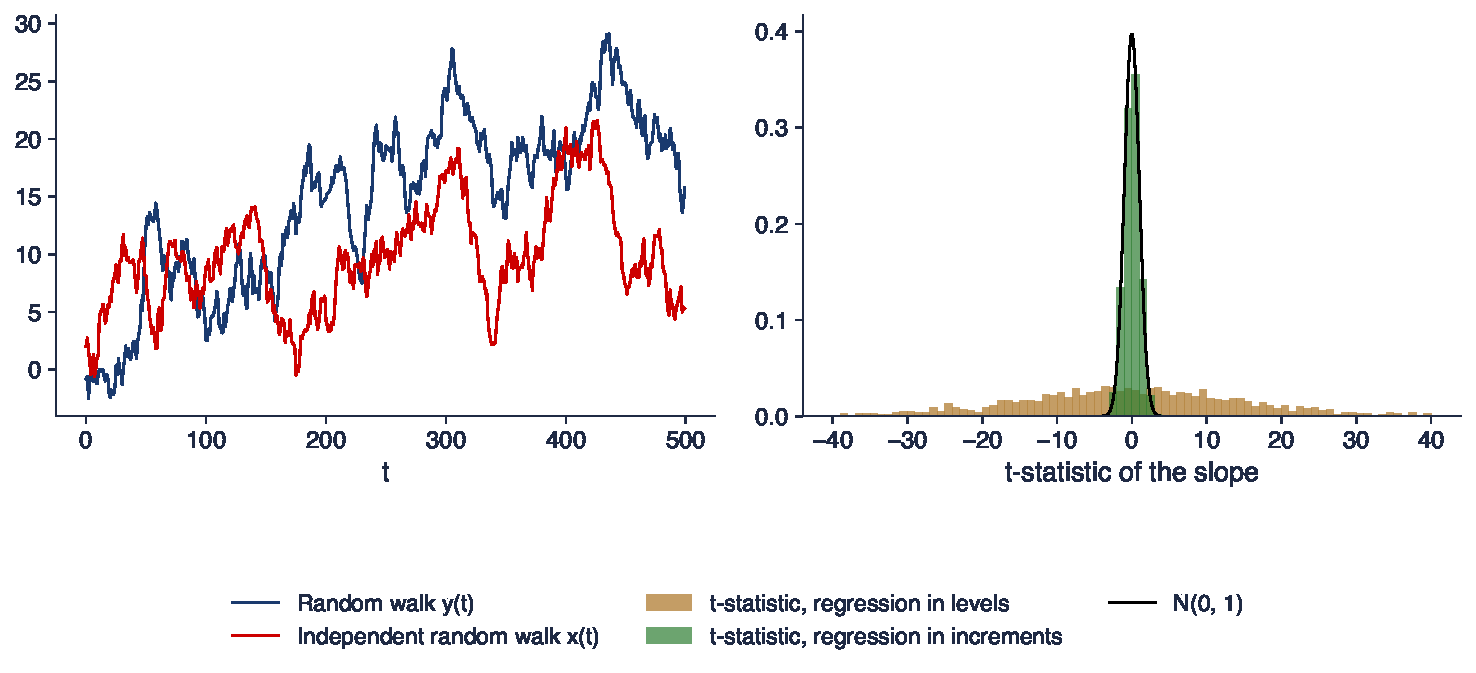
\includegraphics[width=0.97\textwidth,height=0.54\textheight,keepaspectratio]{sfm_ch7_spurious.pdf}
\end{center}
\vspace{-0.25cm}
\begin{itemize}
    \item Estimăm regresia unui mers aleator pe altul, independent ($T = 500$, 2\,000 de repetări) \refGN: $|t| > 1{,}96$ în 90\% din cazuri, $R^2$ median $= 0{,}17$
    \item Pe diferențe: $|t| > 1{,}96$ în 5{,}5\% din cazuri, cum este de așteptat; lecția: testați existența rădăcinii unitare înainte de a estima regresii în niveluri ($|t| > 40$ în 2{,}6\% din cazuri, valori care nu apar în grafic)
\end{itemize}
\sfmquantlet{Ch_07}{SFM_ch7_unit_roots}
\end{frame}

\begin{frame}{Testul Dickey--Fuller}
\itemsize{\small}
\begin{itemize}
    \item Scădem $p_{t-1}$: $\Delta p_t = c + \gamma\, p_{t-1} + \varepsilon_t$ cu $\gamma = \phi - 1$ \refDF
    \begin{itemize}
        \item $H_0$: $\gamma = 0$ (rădăcină unitară); $H_1$: $\gamma < 0$ (staționară); un test unilateral
        \item statistica: $\tau = \hat\gamma/\mathrm{SE}(\hat\gamma)$, raportul $t$ obișnuit din OLS (ordinary least squares, metoda celor mai mici pătrate)
    \end{itemize}
    \item În ipoteza $H_0$, $\tau$ \textbf{nu} urmează o lege $t$ sau Normală: valorile ei critice sînt mai negative
    \begin{itemize}
        \item valorile critice de 5\% \refMacKinnon: $-2{,}86$ cu constantă, $-3{,}41$ cu constantă și tendință (distribuția Normală: $-1{,}645$)
    \end{itemize}
    \item Trei specificații: fără constantă; constanta $c$; constantă și tendință $c + bt$
    \begin{itemize}
        \item prețurile logaritmice cresc în timp: folosim constantă și tendință; randamentele: doar constantă
    \end{itemize}
\end{itemize}
\end{frame}

\begin{frame}{Testul augmentat și un exemplu lucrat}
\itemsize{\small}
\begin{itemize}
    \item \textbf{ADF} (augmented Dickey--Fuller, Dickey--Fuller augmentat) \refSD: adăugăm diferențe decalate ca să eliminăm autocorelația din $\varepsilon_t$
    \begin{itemize}
        \item $\Delta p_t = c + bt + \gamma\, p_{t-1} + \sum_{j=1}^{L} \delta_j \Delta p_{t-j} + \varepsilon_t$; același $\tau$, aceleași valori critice
        \item $L$ ales prin AIC (Akaike information criterion, criteriul informațional Akaike, \sfmchlink{https://danpele.github.io/SFM/RO/Cursuri/capitol6_selectia_modelului_managementul_riscului.pdf}{Capitolul 6}), cel mult $12(T/100)^{1/4}$
    \end{itemize}
    \item \textbf{Exemplu lucrat}: prețul logaritmic BET, constantă, fără decalaje, $T = 7\,243$
    \begin{itemize}
        \item OLS: $\hat\gamma = -0{,}00001$, $\mathrm{SE}(\hat\gamma) = 0{,}00016$
        \item $\tau = -0{,}00001/0{,}00016 = -0{,}09 > -2{,}86$: nu respingem rădăcina unitară
        \item un test $t$ obișnuit (valoarea critică $-1{,}645$) ar fi respins-o: distribuția greșită dă răspunsul greșit
    \end{itemize}
\end{itemize}
\end{frame}

\begin{frame}{Phillips--Perron și KPSS}
\itemsize{\small}
\begin{itemize}
    \item \textbf{PP} (Phillips--Perron) \refPP: regresia Dickey--Fuller fără decalaje; $\tau$ este corectat pentru autocorelație și heteroscedasticitate
    \begin{itemize}
        \item corecția folosește o varianță pe termen lung cu ponderi Bartlett \refNW; aceeași $H_0$ și aceleași valori critice ca ADF
    \end{itemize}
    \item \textbf{KPSS} (Kwiatkowski--Phillips--Schmidt--Shin) \refKPSS: ipotezele sînt \textbf{inversate}
    \begin{itemize}
        \item $H_0$: staționară (în jurul unei constante sau al unei tendințe); $H_1$: rădăcină unitară
        \item $\mathrm{KPSS} = \sum_{t=1}^{T} S_t^2/(T^2\hat\lambda^2)$, $S_t$ sumele parțiale ale reziduurilor, $\hat\lambda^2$ varianța lor pe termen lung
        \item respingem staționaritatea dacă $\mathrm{KPSS} > 0{,}463$ (constantă) sau $> 0{,}146$ (tendință), la 5\%
    \end{itemize}
    \item Folosiți-le pe amîndouă: ADF/PP întreabă „există dovezi împotriva rădăcinii unitare?”; KPSS întreabă „există dovezi împotriva staționarității?”
    \begin{itemize}
        \item ADF nu respinge și KPSS respinge: $I(1)$; ADF respinge și KPSS nu: $I(0)$; ambele resping sau niciunul nu respinge: neconcludent
    \end{itemize}
\end{itemize}
\end{frame}

\begin{frame}{BET: prețul logaritmic și randamentele}
\itemsize{\footnotesize}
\begin{center}
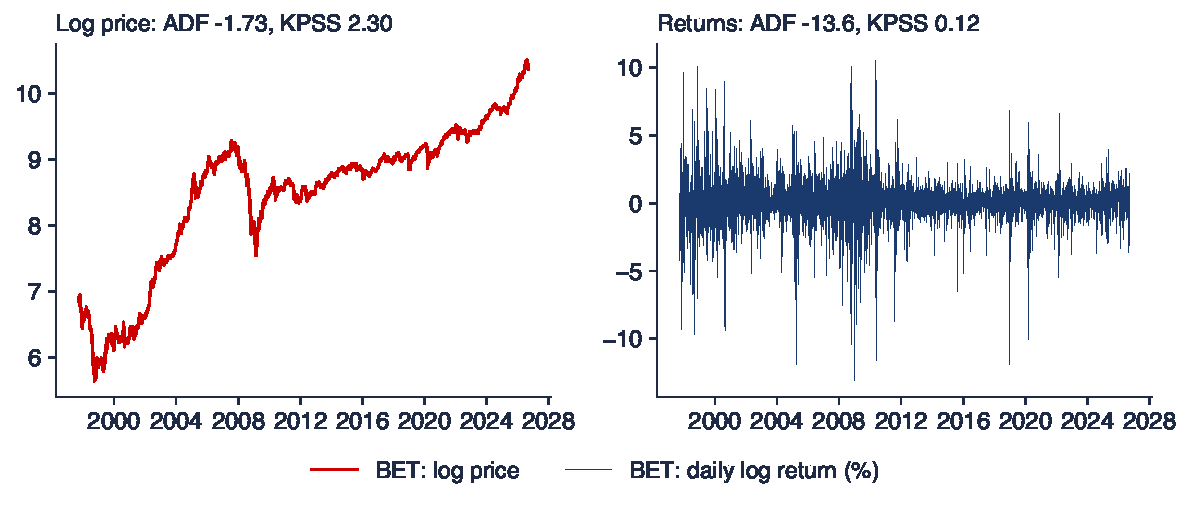
\includegraphics[width=0.97\textwidth,height=0.52\textheight,keepaspectratio]{sfm_ch7_unit_root_bet.pdf}
\end{center}
\vspace{-0.25cm}
\begin{itemize}
    \item Prețul logaritmic: ADF $-1{,}73$ (p = 0{,}736), KPSS $2{,}30$ (p $<$\,0{,}01): rădăcină unitară, nestaționar
    \item Randamentele: ADF $-13{,}65$ (p $<$\,0{,}001), KPSS $0{,}12$ (p $>$\,0{,}10): staționare
    \item Căderea din 2008 pare o abatere temporară, dar testele indică șocuri permanente, fără revenire la o dreaptă de tendință
\end{itemize}
\sfmquantlet{Ch_07}{SFM_ch7_unit_roots}
\end{frame}

\begin{frame}{Teste de rădăcină unitară pe prețuri și randamente}
\itemsize{\footnotesize}
\begin{center}
\scriptsize
\begin{tabular}{lrrrrrr}
\toprule
& \multicolumn{3}{c}{\textbf{preț logaritmic} (constantă, tendință)} & \multicolumn{3}{c}{\textbf{randamente} (constantă)} \\ & ADF & PP & KPSS & ADF & PP & KPSS \\
\midrule
S\&P 500 & ${-1{,}47}$ & ${-1{,}57}$ & ${2{,}23}$ & ${-17{,}61}$ & ${-105{,}05}$ & ${0{,}12}$ \\
DAX & ${-2{,}69}$ & ${-2{,}65}$ & ${0{,}94}$ & ${-23{,}30}$ & ${-97{,}40}$ & ${0{,}04}$ \\
BET & ${-1{,}73}$ & ${-1{,}54}$ & ${2{,}30}$ & ${-13{,}65}$ & ${-74{,}47}$ & ${0{,}12}$ \\
Bitcoin & ${-1{,}48}$ & ${-1{,}54}$ & ${1{,}81}$ & ${-20{,}16}$ & ${-67{,}84}$ & ${0{,}13}$ \\
TLV & ${-3{,}46}$ & ${-3{,}35}$ & ${0{,}57}$ & ${-12{,}96}$ & ${-60{,}79}$ & ${0{,}23}$ \\
SNP & ${-0{,}80}$ & ${-0{,}74}$ & ${2{,}50}$ & ${-19{,}50}$ & ${-62{,}71}$ & ${0{,}29}$ \\
BRD & ${-2{,}18}$ & ${-2{,}19}$ & ${1{,}64}$ & ${-59{,}46}$ & ${-59{,}53}$ & ${0{,}29}$ \\
TGN & ${-0{,}96}$ & ${-0{,}92}$ & ${0{,}71}$ & ${-39{,}90}$ & ${-57{,}83}$ & ${0{,}22}$ \\
\bottomrule
\end{tabular}
\end{center}
\begin{itemize}
    \item Valori critice de 5\%: ADF și PP $-3{,}41$ (tendință), $-2{,}86$ (constantă); KPSS $0{,}146$ (tendință), $0{,}463$ (constantă)
    \item Prețurile logaritmice: nicio respingere ADF/PP cu excepția TLV (ADF p = 0{,}044); KPSS respinge staționaritatea peste tot: prețurile sînt $I(1)$
    \item Randamentele: ADF și PP resping puternic; KPSS nu respinge niciodată (p $>$\,0{,}10): randamentele sînt $I(0)$
\end{itemize}\sfmquantlet{Ch_07}{SFM_ch7_unit_roots}
\end{frame}

\begin{frame}{O rădăcină unitară nu dovedește eficiența}
\itemsize{\small}
\begin{itemize}
    \item O rădăcină unitară în prețuri este \textbf{necesară} pentru un mers aleator, dar \textbf{nu suficientă}
    \begin{itemize}
        \item exemplu: $r_t = 0{,}3\,r_{t-1} + \varepsilon_t$ face din $p_t$ o serie $I(1)$ ale cărei creșteri sînt previzibile
        \item ADF nu o poate deosebi de un mers aleator; BET are rădăcină unitară și randamente autocorelate
    \end{itemize}
    \item Un preț staționar (fără rădăcină unitară) ar contrazice eficiența: prețurile ar reveni la un nivel previzibil
    \begin{itemize}
        \item TLV: ADF respinge la 5\% cu tendință, iar KPSS respinge și el: un caz neconcludent, nu o regulă profitabilă
    \end{itemize}
    \item Testele de rădăcină unitară au putere mică împotriva unui $\phi$ apropiat de 1: întrebarea eficienței privește creșterile și cere teste pe randamente
\end{itemize}
\end{frame}

\begin{frame}{Recapitulare: rădăcini unitare}
\itemsize{\small}
\begin{itemize}
    \item $I(1)$: șocurile sînt permanente; $I(0)$: șocurile se sting; mers aleator = prețuri $I(1)$, randamente $I(0)$
    \item ADF și PP: $H_0$ rădăcină unitară, valori critice Dickey--Fuller; KPSS: $H_0$ staționaritate
    \item Datele noastre: prețuri logaritmice $I(1)$, randamente $I(0)$; regresiile în nivel pot fi false
    \item Rădăcina unitară este necesară, nu suficientă, pentru un mers aleator
\end{itemize}
\end{frame}


%=============================================================================
\section{Testul variance ratio}
%=============================================================================

\begin{frame}{Ideea raportului varianțelor}
\itemsize{\small}
\begin{itemize}
    \item În ipoteza de mers aleator, $\mathrm{Var}(r_t(q)) = q\,\mathrm{Var}(r_t)$; \textbf{VR} (variance ratio, raportul varianțelor) compară cei doi termeni
    \begin{itemize}
        \item $\mathrm{VR}(q) = \dfrac{\mathrm{Var}(r_t(q))}{q\,\mathrm{Var}(r_t)} = 1 + 2\sum_{k=1}^{q-1}\Big(1 - \dfrac{k}{q}\Big)\rho(k)$ \refLM, \refCLM
    \end{itemize}
    \item Interpretarea valorii
    \begin{itemize}
        \item $\mathrm{VR}(q) = 1$: mers aleator (RW1, RW2, RW3 dau toate 1)
        \item $\mathrm{VR}(q) > 1$: autocorelație pozitivă, \textbf{momentum} (mișcările continuă)
        \item $\mathrm{VR}(q) < 1$: autocorelație negativă, \textbf{mean reversion} (revenire la medie: mișcările sînt parțial anulate)
    \end{itemize}
    \item Un singur număr rezumă $q - 1$ autocorelații cu ponderi descrescătoare: mai multă putere împotriva autocorelațiilor mici și persistente
\end{itemize}
\end{frame}

\begin{frame}{Exemplu lucrat: VR din ACF-ul S\&P 500}
\itemsize{\small}
\begin{itemize}
    \item $\hat\rho(1), \dots, \hat\rho(4)$ pentru S\&P 500: $-0{,}079$; $-0{,}004$; $-0{,}006$; $-0{,}022$
    \begin{itemize}
        \item $q = 2$: $\mathrm{VR}(2) = 1 + \hat\rho(1) = 0{,}921$
        \item $q = 5$: ponderile $2(1 - k/5) = 1{,}6;\ 1{,}2;\ 0{,}8;\ 0{,}4$: $\mathrm{VR}(5) = 1 + 1{,}6\hat\rho(1) + 1{,}2\hat\rho(2) + 0{,}8\hat\rho(3) + 0{,}4\hat\rho(4) = 0{,}855$
    \end{itemize}
    \item Estimatorul Lo--MacKinlay pe aceleași date: $\mathrm{VR}(2) = 0{,}922$, $\mathrm{VR}(5) = 0{,}856$
    \begin{itemize}
        \item aproape aceleași cifre: cele două forme diferă doar prin corecții de eșantion mic
    \end{itemize}
    \item Interpretare: varianța săptămînală reprezintă circa $0{,}856$ din suma a cinci varianțe zilnice: mișcările zilnice ale S\&P 500 sînt parțial anulate într-o săptămînă
\end{itemize}
\end{frame}

\begin{frame}{Lo și MacKinlay (1988): estimator și teste}
\itemsize{\footnotesize}
\begin{columns}[T]
\begin{column}{0.66\textwidth}
\begin{itemize}
    \item Cu $T$ randamente, media $\hat\mu$ și sume pe $q$ zile suprapuse \refLM:
    \begin{itemize}
        \item $\hat\sigma_a^2 = \frac{1}{T-1}\sum_t (r_t - \hat\mu)^2$, \quad $\hat\sigma_c^2(q) = \frac{1}{m}\sum_t (r_t(q) - q\hat\mu)^2$
        \item $m = q(T - q + 1)(1 - q/T)$ corectează deplasarea; $\widehat{\mathrm{VR}}(q) = \hat\sigma_c^2(q)/\hat\sigma_a^2$
    \end{itemize}
    \item Testul \textbf{homoscedastic} (RW1): $Z(q) = \dfrac{\widehat{\mathrm{VR}}(q) - 1}{\sqrt{2(2q-1)(q-1)/(3qT)}} \approx N(0, 1)$
    \item Testul \textbf{robust} (RW3, martingal): $Z^*(q) = \dfrac{\widehat{\mathrm{VR}}(q) - 1}{\sqrt{\hat\theta(q)/T}} \approx N(0, 1)$
    \begin{itemize}
        \item $\hat\theta(q) = \sum_{j=1}^{q-1}\big[2(q-j)/q\big]^2\hat\delta(j)$, cu $\hat\delta(j)$ din banda ACF robustă
    \end{itemize}
\end{itemize}
\end{column}
\begin{column}{0.30\textwidth}
\centering
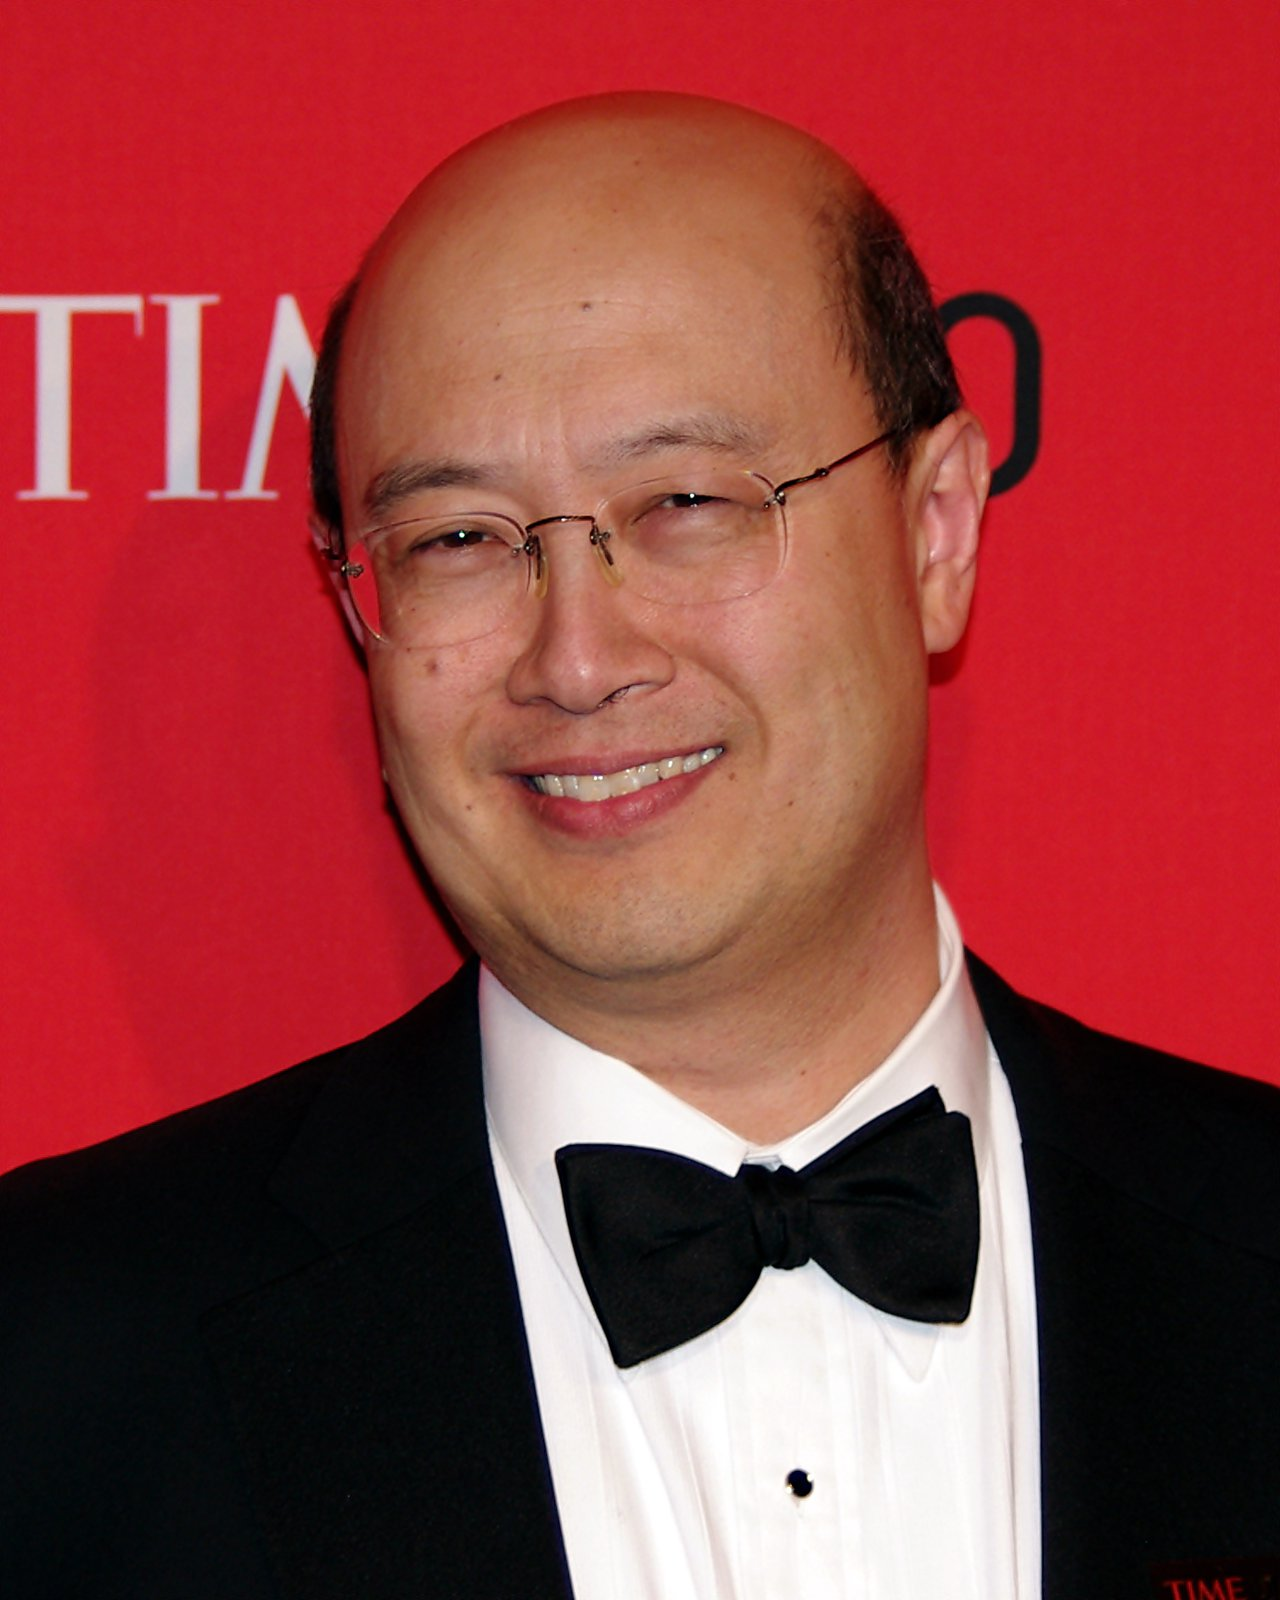
\includegraphics[height=0.40\textheight]{ch7_lo_2012.jpg}\\[1mm]
\imgcap{Andrew W. Lo, MIT}
\imgcredit{https://commons.wikimedia.org/wiki/File:Andrew_Lo_2012_Shankbone_2.JPG}{Foto: David Shankbone (2012); CC BY 3.0; Wikimedia Commons}
\end{column}
\end{columns}\sfmquantlet{Ch_07}{SFM_ch7_variance_ratio}
\end{frame}

\begin{frame}{Necesitatea testului robust: o verificare Monte Carlo}
\itemsize{\footnotesize}
\begin{center}
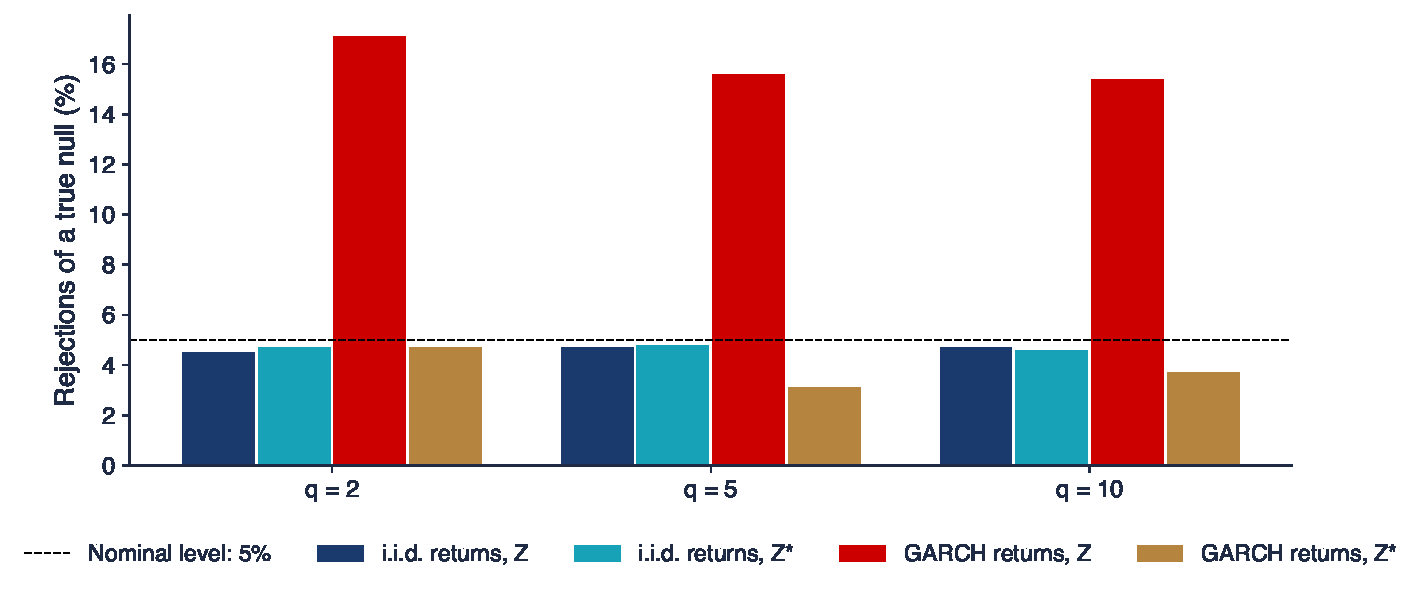
\includegraphics[width=0.97\textwidth,height=0.48\textheight,keepaspectratio]{sfm_ch7_vr_size.pdf}
\end{center}
\vspace{-0.25cm}
\begin{itemize}
    \item 1\,000 de eșantioane de $T = 2000$ de randamente cu $H_0$ adevărată: Normale i.i.d.\ și GARCH(1,1) ($\alpha = 0{,}12$, $\beta = 0{,}86$), adică necorelate, dar cu volatility clustering
    \item i.i.d.: ambele resping circa 5\%; GARCH: $Z(2)$ respinge în 17{,}1\% din cazuri, $Z^*(2)$ doar în 4{,}7\%
    \item \textbf{Mărimea} unui test: cît de des respinge o $H_0$ adevărată; $Z$ „găsește” o ineficiență care nu este decît volatility clustering
\end{itemize}
\sfmquantlet{Ch_07}{SFM_ch7_variance_ratio}
\end{frame}

\begin{frame}{Rapoarte ale varianțelor pentru orizonturi de 2--40 de zile}
\itemsize{\footnotesize}
\begin{center}
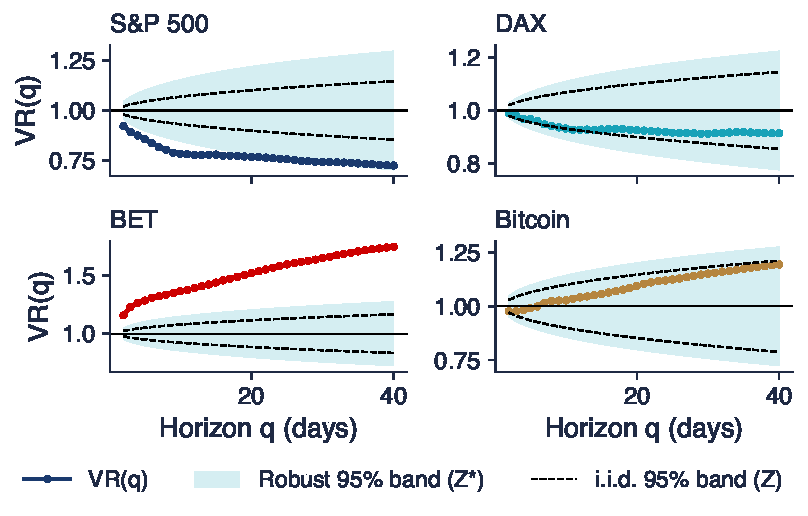
\includegraphics[width=0.97\textwidth,height=0.58\textheight,keepaspectratio]{sfm_ch7_vr_profile.pdf}
\end{center}
\vspace{-0.25cm}
\begin{itemize}
    \item S\&P 500: VR scade sub 1 la orice orizont (mean reversion); BET: VR crește pînă la circa 1{,}517 la 20 de zile și peste (momentum)
    \item DAX și Bitcoin: în interiorul benzii robuste (zona umbrită) la orice orizont; banda i.i.d.\ (linia întreruptă) este mult mai îngustă
\end{itemize}
\sfmquantlet{Ch_07}{SFM_ch7_variance_ratio}
\end{frame}

\begin{frame}{Rapoarte ale varianțelor și teste robuste}
\itemsize{\footnotesize}
\begin{center}
\scriptsize
\begin{tabular}{lrrrrrrrr}
\toprule
& VR(2) & VR(5) & VR(10) & VR(20) & $Z^*(2)$ & $Z^*(5)$ & $Z^*(10)$ & $Z^*(20)$ \\
\midrule
S\&P 500 & $0{,}922$ & $0{,}856$ & $0{,}783$ & $0{,}767$ & ${-3{,}37}$ & ${-2{,}76}$ & ${-2{,}73}$ & ${-2{,}06}$ \\
DAX & $0{,}990$ & $0{,}968$ & $0{,}932$ & $0{,}925$ & ${-0{,}61}$ & ${-0{,}88}$ & ${-1{,}21}$ & ${-0{,}91}$ \\
BET & $1{,}156$ & $1{,}283$ & $1{,}362$ & $1{,}517$ & ${5{,}99}$ & ${5{,}25}$ & ${4{,}74}$ & ${4{,}94}$ \\
Bitcoin & $0{,}977$ & $0{,}991$ & $1{,}027$ & $1{,}094$ & ${-0{,}88}$ & ${-0{,}19}$ & ${0{,}37}$ & ${0{,}91}$ \\
TLV & $1{,}009$ & $0{,}997$ & $0{,}954$ & $0{,}995$ & ${0{,}34}$ & ${-0{,}04}$ & ${-0{,}48}$ & ${-0{,}04}$ \\
SNP & $0{,}985$ & $0{,}960$ & $0{,}975$ & $1{,}038$ & ${-0{,}53}$ & ${-0{,}68}$ & ${-0{,}29}$ & ${0{,}32}$ \\
BRD & $1{,}032$ & $1{,}083$ & $1{,}078$ & $1{,}107$ & ${1{,}28}$ & ${1{,}55}$ & ${0{,}97}$ & ${0{,}96}$ \\
TGN & $1{,}055$ & $1{,}150$ & $1{,}142$ & $1{,}166$ & ${2{,}05}$ & ${2{,}60}$ & ${1{,}69}$ & ${1{,}44}$ \\
\bottomrule
\end{tabular}
\end{center}
\begin{itemize}
    \item $|Z^*| > 1{,}96$: respingem mersul aleator la 5\% pentru acel orizont
    \item S\&P 500: mean reversion semnificativ la toate cele patru orizonturi; BET: momentum semnificativ la toate patru
    \item Transgaz: $Z^*(2) = 2{,}05$ și $Z^*(5) = 2{,}60$; DAX, Bitcoin, TLV, SNP, BRD: nicio respingere
    \item Atenție: sînt opt teste simultane pe fiecare serie, deci unele orizonturi „semnificative” apar din întîmplare
\end{itemize}\sfmquantlet{Ch_07}{SFM_ch7_variance_ratio}
\end{frame}

\begin{frame}{Mai multe orizonturi deodată: testul Chow--Denning}
\itemsize{\small}
\begin{itemize}
    \item Testarea separată pentru $q = 2, 5, 10, 20$ la 5\% crește mult probabilitatea de a obține cel puțin o respingere falsă
    \begin{itemize}
        \item pentru 4 teste independente: $1 - 0{,}95^4 = 18{,}5\%$
    \end{itemize}
    \item Statistica \textbf{CD} (Chow--Denning) \refCD: $\mathrm{CD} = \max_{i} |Z^*(q_i)|$, $i = 1, \dots, m$
    \begin{itemize}
        \item valoarea critică din distribuția modulului maxim studentizat: $P(\mathrm{CD} \le c) = (2\Phi(c) - 1)^m$
        \item $m = 4$, 5\%: $c = 2{,}49$ în loc de $1{,}96$; $\Phi$: funcția de repartiție Normală standard
    \end{itemize}
    \item Respingem mersul aleator dacă cel mai mare $|Z^*|$ depășește $2{,}49$: o singură decizie pentru toate orizonturile
\end{itemize}
\end{frame}

\begin{frame}{O alegere automată a orizontului}
\itemsize{\small}
\begin{itemize}
    \item Orizontul $q$ poate fi ales din date: testul VR automat \refChoi
    \begin{itemize}
        \item $\mathrm{VR}(k) = 1 + 2\sum_{i=1}^{T-1} w(i/k)\,\hat\rho(i)$, cu ponderi $w$ care scad lin (nucleul spectral pătratic) \refAndrews
        \item lățimea de bandă $k$ crește cu autocorelația de ordinul 1 și cu $T$; statistica $\sqrt{T/k}\,(\mathrm{VR}(k) - 1)/\sqrt2 \approx N(0, 1)$
    \end{itemize}
    \item p-valoare prin \textbf{wild bootstrap} \refKimB: reeșantionăm $r_t^* = \eta_t(r_t - \bar r)$ cu $\eta_t \sim N(0, 1)$, de 500 de ori
    \begin{itemize}
        \item fiecare $r_t^*$ păstrează mărimea lui $r_t$ (volatilitatea), dar pierde orice autocorelație: o distribuție nulă robustă
    \end{itemize}
    \item Trei instrumente, o întrebare: $Z^*(q)$ pentru un orizont ales, CD pentru o mulțime de orizonturi, testul automat pentru un orizont ales de date
\end{itemize}
\end{frame}

\begin{frame}{Teste comune și automate pe date reale}
\itemsize{\footnotesize}
\begin{center}
\scriptsize
\begin{tabular}{lrrrrrr}
\toprule
& $T$ & CD & p & $\hat k$ & VR automat & p (bootstrap) \\
\midrule
S\&P 500 & 9\,240 & $3{,}37$ & 0{,}003 & $3{,}7$ & ${-5{,}21}$ & 0{,}006 \\
DAX & 9\,288 & $1{,}21$ & 0{,}644 & $1{,}7$ & ${-0{,}39}$ & 0{,}608 \\
BET & 7\,243 & $5{,}99$ & $<$\,0{,}001 & $5{,}6$ & ${8{,}86}$ & $<$\,0{,}001 \\
Bitcoin & 4\,384 & $0{,}91$ & 0{,}835 & $2{,}0$ & ${-1{,}01}$ & 0{,}352 \\
TLV & 3\,788 & $0{,}48$ & 0{,}981 & $1{,}5$ & ${0{,}31}$ & 0{,}718 \\
SNP & 3\,815 & $0{,}68$ & 0{,}937 & $1{,}7$ & ${-0{,}53}$ & 0{,}562 \\
BRD & 3\,771 & $1{,}55$ & 0{,}403 & $2{,}3$ & ${1{,}58}$ & 0{,}152 \\
TGN & 3\,725 & $2{,}60$ & 0{,}037 & $3{,}0$ & ${3{,}78}$ & 0{,}004 \\
\bottomrule
\end{tabular}
\end{center}
\begin{itemize}
    \item Ambele teste resping pentru S\&P 500, BET și Transgaz; niciunul nu respinge pentru DAX, Bitcoin, TLV, SNP și BRD
    \item $\hat k$ este mare unde prima autocorelație este mare (BET $5{,}6$) și mic unde ea este aproape 0 (DAX $1{,}7$)
    \item Interpretare: respingerea nu înseamnă profit: o autocorelație de $-0{,}079$ explică mai puțin de 1\% din varianța randamentului de mîine; costurile de tranzacționare absorb cea mai mare parte
\end{itemize}\sfmquantlet{Ch_07}{SFM_ch7_variance_ratio}
\end{frame}

\begin{frame}{Recapitulare: testul variance ratio}
\itemsize{\small}
\begin{itemize}
    \item $\mathrm{VR}(q) = 1 + 2\sum_{k<q}(1 - k/q)\rho(k)$; $> 1$ momentum, $< 1$ mean reversion
    \item Folosiți $Z^*(q)$: $Z(q)$ homoscedastic respinge prea des în prezența volatility clustering
    \item Mai multe orizonturi: Chow--Denning; orizont ales de date: VR automat cu wild bootstrap
    \item S\&P 500 revine la medie, BET are momentum; DAX, Bitcoin și majoritatea acțiunilor BVB sînt compatibile cu un mers aleator
\end{itemize}
\end{frame}


%=============================================================================
\section{Eficiența pe piețe și în timp}
%=============================================================================

\begin{frame}{Șaisprezece piețe în ultimii zece ani}
\itemsize{\footnotesize}
\begin{center}
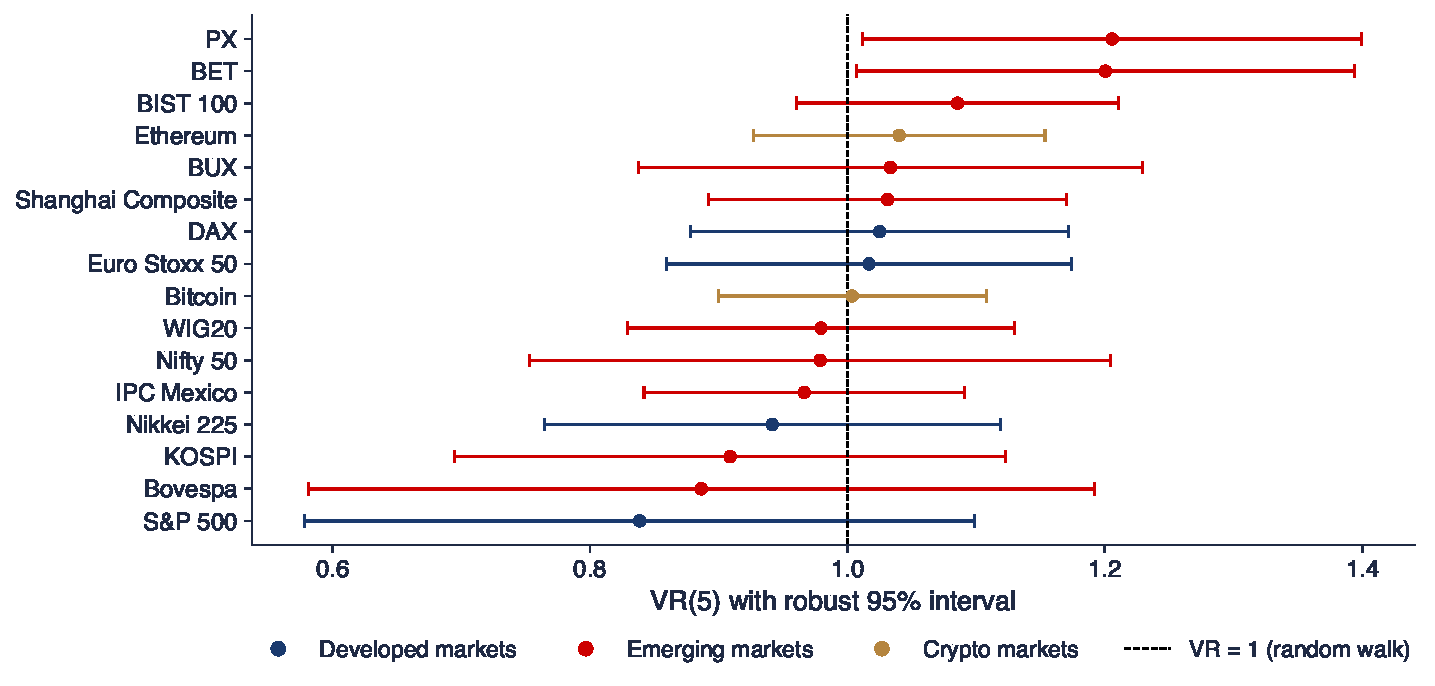
\includegraphics[width=0.97\textwidth,height=0.64\textheight,keepaspectratio]{sfm_ch7_vr_markets.pdf}
\end{center}
\vspace{-0.25cm}
\begin{itemize}
    \item VR(5) cu intervalul robust de 95\%, de la 19 septembrie 2016 pînă la 18 septembrie 2026: piețe dezvoltate, emergente și cripto
\end{itemize}
\sfmquantlet{Ch_07}{SFM_ch7_markets_efficiency}
\end{frame}

\begin{frame}{Interpretarea comparației între piețe}
\itemsize{\small}
\begin{itemize}
    \item Doar două intervale exclud valoarea 1: PX ($Z^*(5) = 2{,}08$) și BET ($Z^*(5) = 2{,}03$), ambele peste 1
    \begin{itemize}
        \item două piețe central-europene mai mici, cu acțiuni mai puțin lichide în indice
    \end{itemize}
    \item \textbf{Multe piețe, multe teste}: 16 teste la 5\% dau, în medie, 0{,}8 respingeri false
    \begin{itemize}
        \item dacă testele ar fi independente, probabilitatea de a obține cel puțin o respingere falsă ar fi $1 - 0{,}95^{16} = 56\%$
        \item Chow--Denning pe patru orizonturi: nicio piață nu respinge la 5\% (BET p = 0{,}159, PX p = 0{,}142)
    \end{itemize}
    \item S\&P 500: VR(5) $= 0{,}84$, cel mai mic, dar cu un interval larg ($Z^* = -1{,}22$): oscilațiile mari din 2020 măresc $\hat\theta$
    \item Bitcoin și Ethereum: VR(5) aproape de 1, ca pe piețele dezvoltate
\end{itemize}\sfmquantlet{Ch_07}{SFM_ch7_markets_efficiency}
\end{frame}

\begin{frame}{Ipoteza piețelor adaptive}
\itemsize{\small}
\begin{columns}[T]
\begin{column}{0.62\textwidth}
\begin{itemize}
    \item \textbf{AMH} (adaptive markets hypothesis, ipoteza piețelor adaptive) \refLo: piețele sînt ecosisteme de investitori care învață și se adaptează
    \begin{itemize}
        \item oportunitățile de profit apar, sînt exploatate și dispar; eficiența se schimbă odată cu mediul
        \item crizele, tehnologia nouă, participanții noi și reglementarea îndepărtează piața de eficiență sau o readuc spre ea
    \end{itemize}
    \item Consecința testabilă: previzibilitatea variază în timp
    \begin{itemize}
        \item dovezi: \refKSL (SUA, un secol de date); \refUM; sinteză: \refLB
    \end{itemize}
    \item Instrumentul: același test pe ferestre mobile
\end{itemize}
\end{column}
\begin{column}{0.34\textwidth}
\centering
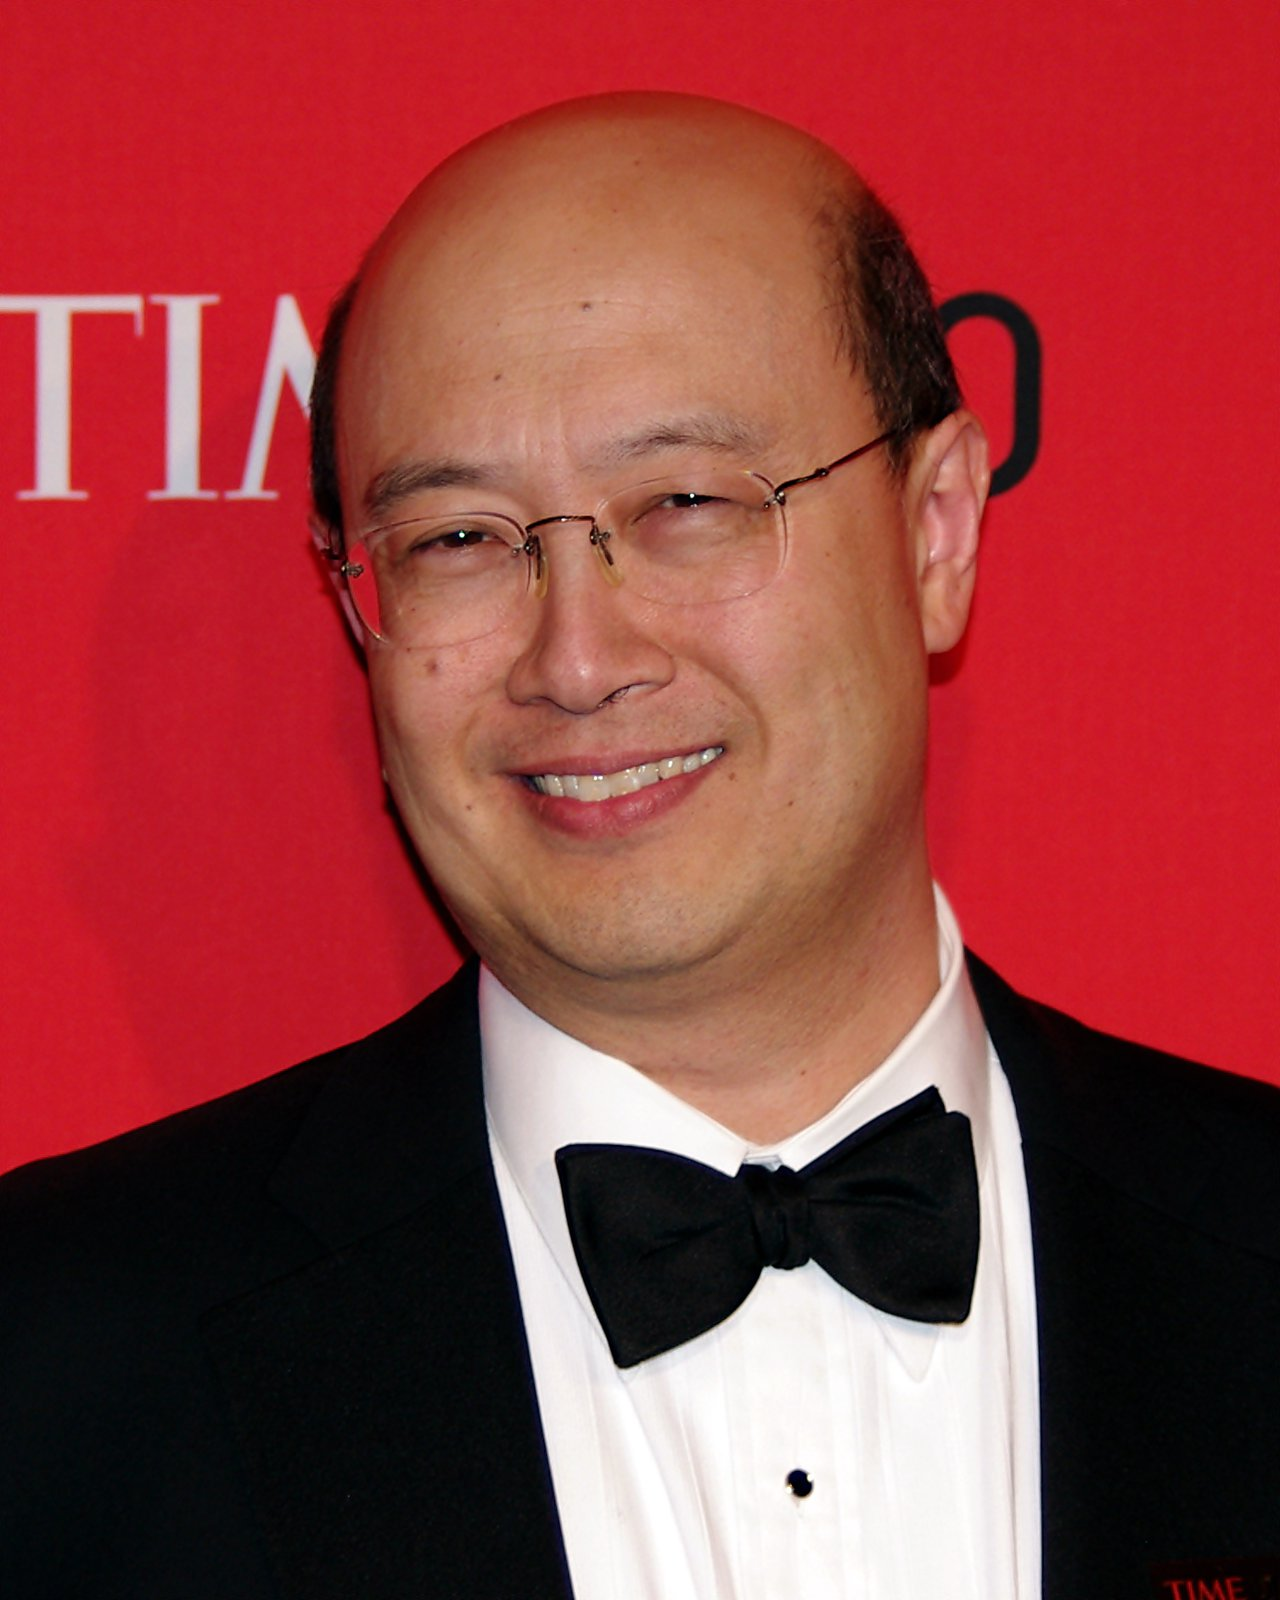
\includegraphics[height=0.42\textheight]{ch7_lo_2012.jpg}\\[1mm]
\imgcap{Andrew W. Lo, autorul AMH}
\imgcredit{https://commons.wikimedia.org/wiki/File:Andrew_Lo_2012_Shankbone_2.JPG}{Foto: David Shankbone (2012); CC BY 3.0; Wikimedia Commons}
\end{column}
\end{columns}
\end{frame}

\begin{frame}{Rapoarte ale varianțelor pe ferestre mobile}
\itemsize{\footnotesize}
\begin{center}
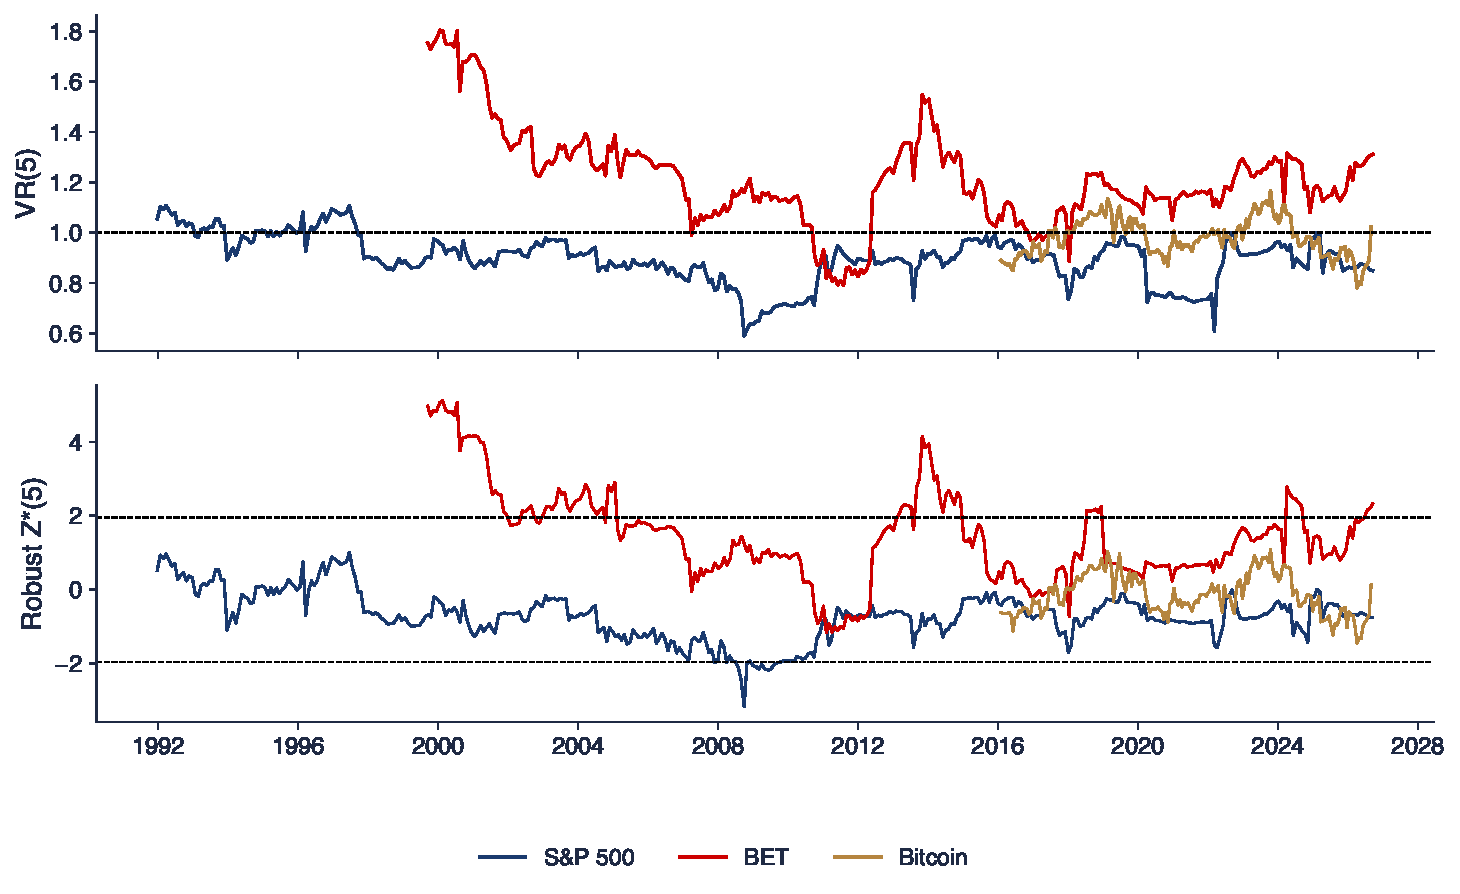
\includegraphics[width=0.97\textwidth,height=0.64\textheight,keepaspectratio]{sfm_ch7_rolling_vr.pdf}
\end{center}
\vspace{-0.25cm}
\begin{itemize}
    \item VR(5) și $Z^*(5)$ pe ferestre de 500 de zile de tranzacționare (circa doi ani), o fereastră nouă la fiecare 21 de zile, datată la sfîrșitul ferestrei
\end{itemize}
\sfmquantlet{Ch_07}{SFM_ch7_adaptive_markets}
\end{frame}

\begin{frame}{Interpretarea rapoartelor varianțelor pe ferestre mobile}
\itemsize{\small}
\begin{itemize}
    \item BET: VR(5) pînă la 1{,}80 în fereastra care se termină în 2000; mai aproape de 1 după 2008, cu excepția unor episoade scurte
    \begin{itemize}
        \item 29\% dintre ferestre resping la 5\%, toate cu VR $> 1$ (momentum)
    \end{itemize}
    \item S\&P 500: VR(5) mai ales sub 1; cel mai mic, 0{,}59, în fereastra care se termină în 2008
    \begin{itemize}
        \item 4\% dintre ferestre resping, toate cu VR $< 1$: revenirile sînt cele mai puternice în crize
    \end{itemize}
    \item Bitcoin: nicio fereastră nu respinge din 2016 (185 de ferestre)
    \item Atenție: ferestrele consecutive au în comun 479 din 500 de zile; ponderea ferestrelor care resping este o descriere, nu un test
\end{itemize}\sfmquantlet{Ch_07}{SFM_ch7_adaptive_markets}
\end{frame}

\begin{frame}{Trei subperioade pentru fiecare piață}
\itemsize{\footnotesize}
\begin{center}
\scriptsize
\begin{tabular}{llrrrrr}
\toprule
& perioada & $T$ & $\hat\rho(1)$ & VR(5) & $Z^*(5)$ & CD p \\
\midrule
BET & 1997--2006 & 2\,306 & ${0{,}270}$ & $1{,}50$ & ${6{,}15}$ & $<$\,0{,}001 \\
BET & 2007--2016 & 2\,516 & ${0{,}066}$ & $1{,}08$ & ${0{,}82}$ & 0{,}262 \\
BET & 2017--2026 & 2\,421 & ${0{,}064}$ & $1{,}20$ & ${2{,}04}$ & 0{,}154 \\
S\&P 500 & 1990--2001 & 3\,025 & ${0{,}017}$ & $0{,}96$ & ${-0{,}62}$ & 0{,}334 \\
S\&P 500 & 2002--2013 & 3\,019 & ${-0{,}100}$ & $0{,}80$ & ${-2{,}53}$ & 0{,}010 \\
S\&P 500 & 2014--2026 & 3\,196 & ${-0{,}124}$ & $0{,}85$ & ${-1{,}30}$ & 0{,}080 \\
Bitcoin & 2014--2017 & 1\,201 & ${0{,}028}$ & $0{,}98$ & ${-0{,}23}$ & 0{,}983 \\
Bitcoin & 2018--2021 & 1\,461 & ${-0{,}058}$ & $0{,}98$ & ${-0{,}21}$ & 0{,}374 \\
Bitcoin & 2022--2026 & 1\,722 & ${-0{,}026}$ & $1{,}01$ & ${0{,}18}$ & 0{,}924 \\
\bottomrule
\end{tabular}
\end{center}
\begin{itemize}
    \item BET: momentum puternic în 1997--2006 ($\hat\rho(1) = 0{,}270$), mult mai slab după aceea; din 2017 VR(5) este tot peste 1, dar testul comun nu respinge
    \item S\&P 500: autocorelația negativă apare după 2002; Bitcoin: nicio respingere în vreuna dintre subperioadele de după 2014; \refUrquhart a găsit ineficiență în primii lui ani
\end{itemize}\sfmquantlet{Ch_07}{SFM_ch7_adaptive_markets}
\end{frame}

\begin{frame}{Previzibilitatea BET în primii ani}
\itemsize{\small}
\begin{columns}[T]
\begin{column}{0.60\textwidth}
\begin{itemize}
    \item \textbf{Tranzacționare redusă} (thin trading): puține tranzacții pe zi la multe acțiuni din indice
    \begin{itemize}
        \item un preț de închidere poate fi vechi de cîteva ore; știrile intră în indice pe parcursul mai multor zile
        \item indicele arată atunci autocorelație pozitivă chiar dacă fiecare acțiune este eficientă
    \end{itemize}
    \item Schimbările de după 2007
    \begin{itemize}
        \item mai multă lichiditate, investitori străini, aderarea la UE, reclasificarea de către FTSE Russell la statutul Secondary Emerging (2020) \refFTSE
    \end{itemize}
    \item Crahurile de la Bursa de Valori București: \refPeleA
\end{itemize}
\end{column}
\begin{column}{0.36\textwidth}
\centering
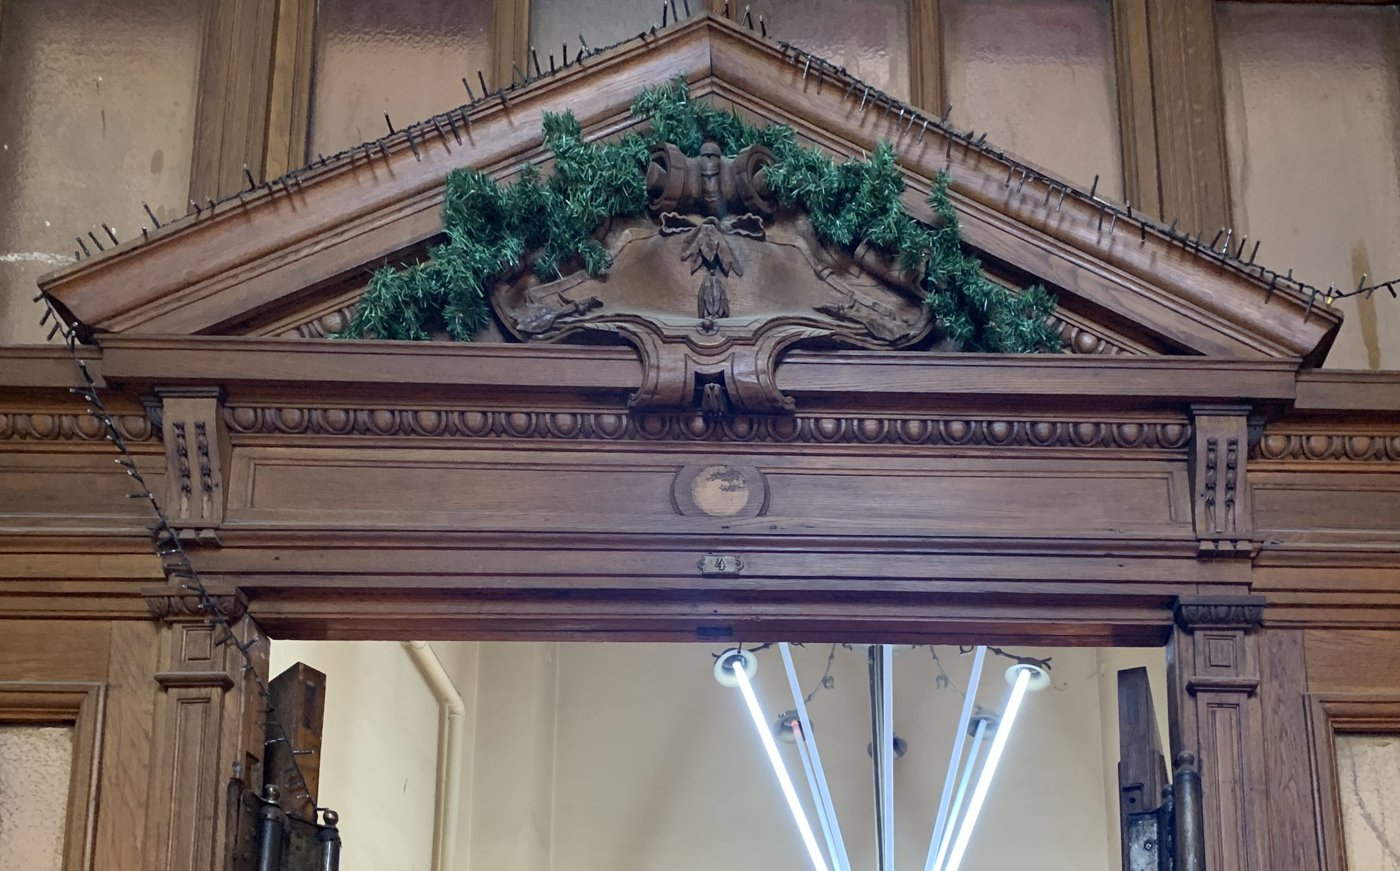
\includegraphics[height=0.32\textheight]{ch5_bvb_palace_2019.jpg}\\[1mm]
\imgcap{Palatul Bursei, București}
\imgcredit{https://commons.wikimedia.org/wiki/File:Stock_Exchange_Palace_(Bucharest).jpg}{Foto: Neoclassicism Enthusiast (2019); CC BY-SA 4.0; Wikimedia Commons}
\end{column}
\end{columns}
\end{frame}

\begin{frame}{Recapitulare: eficiența pe piețe și în timp}
\itemsize{\small}
\begin{itemize}
    \item În ultimii zece ani majoritatea piețelor, inclusiv Bitcoin, sînt compatibile cu un mers aleator
    \item Eficiența se schimbă în timp: AMH; ferestrele mobile o arată, dar se suprapun
    \item BET în primii ani: tranzacționare redusă și momentum; azi: mult mai aproape de un mers aleator
    \item Multe piețe, multe teste: așteptați-vă la cîteva respingeri false
\end{itemize}
\end{frame}


%=============================================================================
\section{Forma semi-tare, forma tare și anomalii}
%=============================================================================

\begin{frame}{Studii de eveniment și forma tare}
\itemsize{\small}
\begin{itemize}
    \item \textbf{Studiu de eveniment} (forma semi-tare) \refMacKinlay, \refCLM, cap.~4: cît de repede absoarbe un preț o știre publică?
    \begin{itemize}
        \item randamentul anormal: randamentul minus randamentul unui model (de exemplu piața); cumulat pe o fereastră în jurul anunțului
        \item piață eficientă: un salt în ziua știrii, fără derivă ulterioară
        \item cercetări recente: cît de repede absorb prețurile futures știrile, măsurat în nanosecunde la Eurex și CME \refPeleB; reacția pieței la actualizările Ethereum \refPeleC
    \end{itemize}
    \item \textbf{Forma tare}: poate cineva cu informație privată să obțină randamente în exces?
    \begin{itemize}
        \item insiderii (managerii care tranzacționează acțiunile propriei companii) pot: de aceea tranzacționarea pe baza informațiilor privilegiate este ilegală
        \item administratorii profesioniști de fonduri, în majoritate, nu pot \refJensen, \refFF
    \end{itemize}
\end{itemize}
\end{frame}

\begin{frame}{Anomalii calendaristice}
\itemsize{\small}
\begin{itemize}
    \item O \textbf{anomalie}: un tipar în randamente pe care modelul de echilibru nu îl explică
    \begin{itemize}
        \item \textbf{efectul de weekend}: randamente mici sau negative lunea \refFrench
        \item \textbf{efectul ianuarie}: randamente mai mari în ianuarie, mai ales la acțiunile mici \refRK
        \item \textbf{efectul de început de lună}: randamente concentrate în jurul primelor zile de tranzacționare ale lunii \refAriel
    \end{itemize}
    \item Durează anomaliile?
    \begin{itemize}
        \item randamentele anomaliilor publicate scad după publicare: investitorii învață \refMP
        \item au fost testate sute de tipare: un tipar nou trebuie să aibă $|t| > 3$, nu 2 \refHLZ
    \end{itemize}
    \item Căutarea repetată în date (data mining): cu destule împărțiri calendaristice, unele vor părea semnificative din întîmplare
\end{itemize}
\end{frame}

\begin{frame}{Randamentele pe zile ale săptămînii: S\&P 500 și BET}
\itemsize{\footnotesize}
\begin{center}
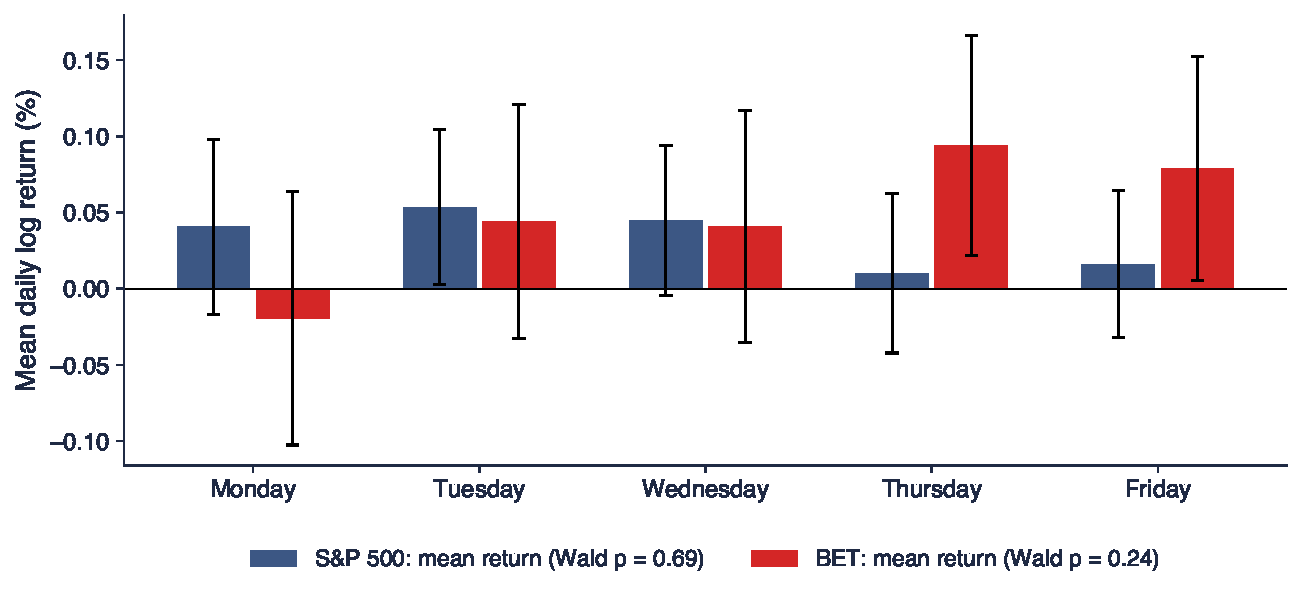
\includegraphics[width=0.97\textwidth,height=0.50\textheight,keepaspectratio]{sfm_ch7_calendar.pdf}
\end{center}
\vspace{-0.25cm}
\begin{itemize}
    \item Randamentul zilnic mediu pe zile ale săptămînii, cu intervale de 95\% (erori standard Newey--West \refNW); testul Wald al mediilor egale: S\&P 500 p = 0{,}69, BET p = 0{,}24
    \item BET lunea: $-0{,}019\%$, singura medie negativă, dar nesemnificativă; ianuarie: BET $0{,}185\%$ pe zi față de $0{,}036\%$ ($t = 1{,}72$, p = 0{,}09); S\&P 500: p = 0{,}59
    \item Niciun efect calendaristic nu rezistă la 5\% în datele noastre
\end{itemize}
\sfmquantlet{Ch_07}{SFM_ch7_calendar_anomalies}
\end{frame}

\begin{frame}{Recapitulare: forma semi-tare, forma tare și anomalii}
\itemsize{\small}
\begin{itemize}
    \item Studiile de eveniment: pe piețele eficiente prețurile reacționează imediat la știrile publice, fără derivă
    \item Forma tare nu este valabilă pentru insideri, dar este aproximativ valabilă pentru administratorii profesioniști de fonduri
    \item Anomaliile calendaristice: slabe în datele noastre și se estompează după publicare
\end{itemize}
\end{frame}


%=============================================================================
\section{AI pentru descoperire științifică}
%=============================================================================

\begin{frame}{O întrebare deschisă}
\itemsize{\small}
\begin{itemize}
    \item \textbf{A devenit BET mai eficient după trecerea României la statutul de piață Secondary Emerging (septembrie 2020)?} \refFTSE
    \begin{itemize}
        \item cinci ani înainte: $\hat\rho(1) = -0{,}002$, VR(5) $= 1{,}12$ ($Z^* = 0{,}80$); cinci ani după: $\hat\rho(1) = 0{,}087$, VR(5) $= 1{,}18$ ($Z^* = 1{,}78$)
        \item diferența celor două VR(5): $z = 0{,}34$: nicio dovadă de schimbare
    \end{itemize}
    \item Întrebarea rămîne deschisă: pandemia COVID-19, noile listări mari și volumele mai mari s-au produs în același timp; care este unitatea potrivită de analiză, indicele sau fiecare acțiune?
    \item Instrumentele AI pot accelera un astfel de studiu; nu înlocuiesc verificarea lui \refWang
\end{itemize}\sfmquantlet{Ch_07}{SFM_ch7_adaptive_markets}
\end{frame}

\begin{frame}{Contribuția posibilă a AI}
\itemsize{\small}
\begin{itemize}
    \item \textbf{Literatura}: o listă a studiilor despre eficiența piețelor din Europa Centrală și de Est și a testelor folosite în ele
    \item \textbf{Cod}: o primă versiune a testelor Lo--MacKinlay și VR automat pe ferestre mobile pentru acțiunile din BET, cu p-valori wild bootstrap
    \item \textbf{Robustețe}: alte ferestre, alte orizonturi, BET-TR în loc de BET, volumul tranzacțiilor ca variabilă de control
    \item Exemplu de prompt
    \begin{itemize}
        \item \aiprompt{Write a Python function that computes the Lo-MacKinlay variance ratio VR(5) and the heteroskedasticity-robust z-statistic for daily BET log returns on rolling 500-day windows, and test whether the mean VR differs before and after 21 September 2020.}
    \end{itemize}
\end{itemize}
\end{frame}

\begin{frame}{Verificări necesare}
\itemsize{\small}
\begin{itemize}
    \item Statistica: $Z^*$ robust, nu $Z$ homoscedastic; o ciornă care folosește $Z$ va „găsi” ineficiență
    \item Randamentele logaritmice ale indicelui, nu nivelurile prețurilor; un test de rădăcină unitară pe randamente nu este un test de eficiență
    \item Ferestrele mobile se suprapun: un test $t$ pe media statisticilor mobile tratează valori dependente ca independente
    \item Data evenimentului și fereastra se fixează înainte de a vedea rezultatul
    \item Referințele: fiecare lucrare citată trebuie să existe; verificați DOI-ul
\end{itemize}
\end{frame}

\begin{frame}{Idee de proiect}
\itemsize{\small}
\begin{itemize}
    \item \textbf{Întrebarea}: este piața de la București mai eficientă azi decît în 2015?
    \begin{itemize}
        \item o a doua întrebare: apare schimbarea în indice sau în acțiunile individuale?
        \item date: BET din 1997, BET-TR din 2014, acțiuni BVB (TLV, SNP, BRD, TGN) din 2010 (EODHD)
    \end{itemize}
    \item Pași
    \begin{itemize}
        \item VR(2), VR(5) mobile cu $Z^*$ și testul Chow--Denning pentru indice și pentru fiecare acțiune
        \item comparați 2015--2020 cu 2020--2025 printr-un bootstrap pe blocuri al diferenței
        \item repetați pentru WIG20 și BUX, ca termeni de comparație: s-au schimbat toate în același timp?
    \end{itemize}
    \item Livrabil: un tabel, un grafic și un paragraf despre ce pot și ce nu pot arăta datele
    \item Declarați orice utilizare a instrumentelor AI și enumerați erorile acestora pe care le-ați corectat
\end{itemize}
\end{frame}


%=============================================================================
\section{Rezumat}
%=============================================================================

\begin{frame}{Idei de reținut}
\itemsize{\small}
\begin{itemize}
    \item Piață eficientă: prețurile reflectă informația; forma slabă = prețurile trecute nu pot fi folosite pentru randamente în exces
    \item Ipoteza nulă potrivită este martingalul (RW3), nu RW1: volatility clustering nu înseamnă ineficiență
    \item Prețurile logaritmice sînt $I(1)$, iar randamentele $I(0)$ în toate seriile noastre; rădăcina unitară, în sine, nu dovedește eficiența
    \item Folosiți teste robuste: $\tilde Q$ și $Z^*(q)$; combinați orizonturile cu Chow--Denning sau lăsați datele să aleagă (VR automat)
    \item Dovezi: S\&P 500 revine ușor la medie, BET avea momentum în primii ani, majoritatea piețelor sînt azi aproape eficiente; eficiența variază în timp
    \item Previzibilitatea statistică nu înseamnă profit: costurile și riscul decid
\end{itemize}
\end{frame}

\begin{frame}{Formule de reținut}
\itemsize{\small}
{\renewcommand{\arraystretch}{1.45}\begin{center}
\scriptsize
\begin{tabular}{ll}
\toprule
\textbf{Mărimea} & \textbf{Formula} \\
\midrule
Mers aleator & $p_t = \mu + p_{t-1} + \varepsilon_t$, \quad $\mathrm{Var}(r_t(q)) = q\sigma^2$ \\
ACF de selecție & $\hat\rho(k) = \sum_t e_te_{t-k}/\sum_t e_t^2$, \quad band $\pm 1{,}96\sqrt{\hat\delta(k)/T}$ \\
Ljung--Box & $Q_{LB}(m) = T(T+2)\sum_{k=1}^m \hat\rho(k)^2/(T-k) \sim \chi^2(m)$ \\
Testul runs & $E[R] = 2n_1n_2/n + 1$, \quad $z = (R - E[R])/\mathrm{sd}(R)$ \\
ADF & $\Delta p_t = c + bt + \gamma p_{t-1} + \sum_j \delta_j\Delta p_{t-j} + \varepsilon_t$, \quad $\tau = \hat\gamma/\mathrm{SE}(\hat\gamma)$ \\
KPSS & $\sum_t S_t^2/(T^2\hat\lambda^2)$, \quad $H_0$: staționaritate \\
VR & $\mathrm{VR}(q) = 1 + 2\sum_{k=1}^{q-1}(1 - k/q)\rho(k)$ \\
Testul VR robust & $Z^*(q) = (\widehat{\mathrm{VR}}(q) - 1)/\sqrt{\hat\theta(q)/T}$, \quad $\hat\theta(q) = \sum_{j<q}[2(q-j)/q]^2\hat\delta(j)$ \\
Chow--Denning & $\max_i |Z^*(q_i)|$, \quad $P(\mathrm{CD} \le c) = (2\Phi(c) - 1)^m$ \\
\bottomrule
\end{tabular}
\end{center}
}
\end{frame}

\begin{frame}{Autoevaluare}
\itemsize{\small}
\begin{itemize}
    \item \textbf{Întrebare}: $\hat\rho(1) = 0{,}10$ și $\hat\rho(k) = 0$ pentru $k \ge 2$; ce ne spune VR(2)?
    \begin{itemize}
        \item \textbf{Răspuns}: $1 + 0{,}10 = 1{,}10$: varianța pe două zile este cu 10\% mai mare decît în cazul unui mers aleator, deci momentum
    \end{itemize}
    \item \textbf{Întrebare}: ADF nu respinge pe prețurile logaritmice, iar KPSS respinge; este piața eficientă?
    \begin{itemize}
        \item \textbf{Răspuns}: știm doar că prețurile sînt $I(1)$; eficiența cere teste pe creșteri (ACF, VR)
    \end{itemize}
    \item \textbf{Întrebare}: $Q_{LB}(10)$ respinge puternic pentru randamentele la pătrat; este respinsă eficiența în formă slabă?
    \begin{itemize}
        \item \textbf{Răspuns}: nu; este vorba de volatility clustering, care respinge RW1 și RW2, nu martingalul
    \end{itemize}
    \item Urmează: Capitolul 8, estimatori de volatilitate și volatility clustering
\end{itemize}
\end{frame}


%=============================================================================
\section{Bibliografie}
%=============================================================================

\begin{frame}{Bibliografie (1/3)}
\itemsize{\tiny}
\begin{itemize}
    \item Andrews, D.W.K. (1991). \href{https://doi.org/10.2307/2938229}{Heteroskedasticity and autocorrelation consistent covariance matrix estimation}. \textit{Econometrica}, 59(3), 817--858.
    \item Ariel, R.A. (1987). \href{https://doi.org/10.1016/0304-405X(87)90066-3}{A monthly effect in stock returns}. \textit{Journal of Financial Economics}, 18(1), 161--174.
    \item Bachelier, L. (1900). \href{https://doi.org/10.24033/asens.476}{Théorie de la spéculation}. \textit{Annales scientifiques de l'École normale supérieure}, 17, 21--86.
    \item Borak, S., Härdle, W.K., López-Cabrera, B. (2013). \href{https://doi.org/10.1007/978-3-642-33929-5}{\textit{Statistics of Financial Markets: Exercises and Solutions}}, 2nd ed. Springer.
    \item Box, G.E.P., Pierce, D.A. (1970). \href{https://doi.org/10.1080/01621459.1970.10481180}{Distribution of residual autocorrelations in autoregressive-integrated moving average time series models}. \textit{Journal of the American Statistical Association}, 65(332), 1509--1526.
    \item Campbell, J.Y., Lo, A.W., MacKinlay, A.C. (1997). \href{https://doi.org/10.1515/9781400830213}{\textit{The Econometrics of Financial Markets}}. Princeton University Press.
    \item Choi, I. (1999). \href{https://doi.org/10.1002/(SICI)1099-1255(199905/06)14:3<293::AID-JAE503>3.0.CO;2-5}{Testing the random walk hypothesis for real exchange rates}. \textit{Journal of Applied Econometrics}, 14(3), 293--308.
    \item Chow, K.V., Denning, K.C. (1993). \href{https://doi.org/10.1016/0304-4076(93)90051-6}{A simple multiple variance ratio test}. \textit{Journal of Econometrics}, 58(3), 385--401.
    \item Dickey, D.A., Fuller, W.A. (1979). \href{https://doi.org/10.1080/01621459.1979.10482531}{Distribution of the estimators for autoregressive time series with a unit root}. \textit{Journal of the American Statistical Association}, 74(366), 427--431.
    \item Escanciano, J.C., Lobato, I.N. (2009). \href{https://doi.org/10.1016/j.jeconom.2009.03.001}{An automatic Portmanteau test for serial correlation}. \textit{Journal of Econometrics}, 151(2), 140--149.
    \item Fama, E.F. (1965). \href{https://doi.org/10.1086/294743}{The behavior of stock-market prices}. \textit{Journal of Business}, 38(1), 34--105.
    \item Fama, E.F. (1970). \href{https://doi.org/10.1111/j.1540-6261.1970.tb00518.x}{Efficient capital markets: a review of theory and empirical work}. \textit{Journal of Finance}, 25(2), 383--417.
    \item Fama, E.F. (1991). \href{https://doi.org/10.1111/j.1540-6261.1991.tb04636.x}{Efficient capital markets: II}. \textit{Journal of Finance}, 46(5), 1575--1617.
    \item Fama, E.F., French, K.R. (2010). \href{https://doi.org/10.1111/j.1540-6261.2010.01598.x}{Luck versus skill in the cross-section of mutual fund returns}. \textit{Journal of Finance}, 65(5), 1915--1947.
    \item Franke, J., Härdle, W.K., Hafner, C.M. (2019). \href{https://doi.org/10.1007/978-3-030-13751-9}{\textit{Statistics of Financial Markets: An Introduction}}, 5th ed. Springer.
    \item French, K.R. (1980). \href{https://doi.org/10.1016/0304-405X(80)90021-5}{Stock returns and the weekend effect}. \textit{Journal of Financial Economics}, 8(1), 55--69.
\end{itemize}
\end{frame}

\begin{frame}{Bibliografie (2/3)}
\itemsize{\tiny}
\begin{itemize}
    \item FTSE Russell (2019). \href{https://www.lseg.com/en/media-centre/press-releases/ftse-russell/2019/ftse-russell-announces-results-country-classification-review-equities-and-fixed-income}{FTSE Russell announces results of country classification review}. Press release, London Stock Exchange Group.
    \item Granger, C.W.J., Newbold, P. (1974). \href{https://doi.org/10.1016/0304-4076(74)90034-7}{Spurious regressions in econometrics}. \textit{Journal of Econometrics}, 2(2), 111--120.
    \item Grossman, S.J., Stiglitz, J.E. (1980). \href{https://ideas.repec.org/a/aea/aecrev/v70y1980i3p393-408.html}{On the impossibility of informationally efficient markets}. \textit{American Economic Review}, 70(3), 393--408.
    \item Harvey, C.R., Liu, Y., Zhu, H. (2016). \href{https://doi.org/10.1093/rfs/hhv059}{\ldots and the cross-section of expected returns}. \textit{Review of Financial Studies}, 29(1), 5--68.
    \item Jensen, M.C. (1968). \href{https://doi.org/10.1111/j.1540-6261.1968.tb00815.x}{The performance of mutual funds in the period 1945--1964}. \textit{Journal of Finance}, 23(2), 389--416.
    \item Kendall, M.G. (1953). \href{https://doi.org/10.2307/2980947}{The analysis of economic time-series, Part I: prices}. \textit{Journal of the Royal Statistical Society, Series A}, 116(1), 11--34.
    \item Kim, J.H. (2009). \href{https://doi.org/10.1016/j.frl.2009.04.003}{Automatic variance ratio test under conditional heteroskedasticity}. \textit{Finance Research Letters}, 6(3), 179--185.
    \item Kim, J.H., Shamsuddin, A., Lim, K.-P. (2011). \href{https://doi.org/10.1016/j.jempfin.2011.08.002}{Stock return predictability and the adaptive markets hypothesis: evidence from century-long U.S. data}. \textit{Journal of Empirical Finance}, 18(5), 868--879.
    \item Kwiatkowski, D., Phillips, P.C.B., Schmidt, P., Shin, Y. (1992). \href{https://doi.org/10.1016/0304-4076(92)90104-Y}{Testing the null hypothesis of stationarity against the alternative of a unit root}. \textit{Journal of Econometrics}, 54(1--3), 159--178.
    \item Lim, K.-P., Brooks, R. (2011). \href{https://doi.org/10.1111/j.1467-6419.2009.00611.x}{The evolution of stock market efficiency over time: a survey of the empirical literature}. \textit{Journal of Economic Surveys}, 25(1), 69--108.
    \item Lin, Y., Găman, A., Wang, Y., Pele, D.T. (2025). \href{https://doi.org/10.2139/ssrn.5176758}{Market responses to Ethereum development milestones: an event study approach}. SSRN Working Paper 5176758.
    \item Ljung, G.M., Box, G.E.P. (1978). \href{https://doi.org/10.1093/biomet/65.2.297}{On a measure of lack of fit in time series models}. \textit{Biometrika}, 65(2), 297--303.
    \item Lo, A.W. (2004). \href{https://doi.org/10.3905/jpm.2004.442611}{The adaptive markets hypothesis}. \textit{Journal of Portfolio Management}, 30(5), 15--29.
    \item Lo, A.W. (2017). \href{https://doi.org/10.1515/9781400887767}{\textit{Adaptive Markets: Financial Evolution at the Speed of Thought}}. Princeton University Press.
    \item Lo, A.W., MacKinlay, A.C. (1988). \href{https://doi.org/10.1093/rfs/1.1.41}{Stock market prices do not follow random walks: evidence from a simple specification test}. \textit{Review of Financial Studies}, 1(1), 41--66.
    \item MacKinlay, A.C. (1997). \href{https://ideas.repec.org/a/aea/jeclit/v35y1997i1p13-39.html}{Event studies in economics and finance}. \textit{Journal of Economic Literature}, 35(1), 13--39.
\end{itemize}
\end{frame}

\begin{frame}{Bibliografie (3/3)}
\itemsize{\tiny}
\begin{itemize}
    \item MacKinnon, J.G. (1996). \href{https://doi.org/10.1002/(SICI)1099-1255(199611)11:6<601::AID-JAE417>3.0.CO;2-T}{Numerical distribution functions for unit root and cointegration tests}. \textit{Journal of Applied Econometrics}, 11(6), 601--618.
    \item Malkiel, B.G. (2003). \href{https://doi.org/10.1257/089533003321164958}{The efficient market hypothesis and its critics}. \textit{Journal of Economic Perspectives}, 17(1), 59--82.
    \item McLean, R.D., Pontiff, J. (2016). \href{https://doi.org/10.1111/jofi.12365}{Does academic research destroy stock return predictability?} \textit{Journal of Finance}, 71(1), 5--32.
    \item Newey, W.K., West, K.D. (1987). \href{https://doi.org/10.2307/1913610}{A simple, positive semi-definite, heteroskedasticity and autocorrelation consistent covariance matrix}. \textit{Econometrica}, 55(3), 703--708.
    \item Pele, D.T., Mazurencu-Marinescu, M. (2012). \href{https://doi.org/10.1016/j.sbspro.2012.09.1030}{Modelling stock market crashes: the case of Bucharest Stock Exchange}. \textit{Procedia -- Social and Behavioral Sciences}, 58, 533--542.
    \item Phillips, P.C.B., Perron, P. (1988). \href{https://doi.org/10.1093/biomet/75.2.335}{Testing for a unit root in time series regression}. \textit{Biometrika}, 75(2), 335--346.
    \item Roberts, H.V. (1959). \href{https://doi.org/10.1111/j.1540-6261.1959.tb00481.x}{Stock-market ``patterns'' and financial analysis: methodological suggestions}. \textit{Journal of Finance}, 14(1), 1--10.
    \item Rozeff, M.S., Kinney, W.R. (1976). \href{https://doi.org/10.1016/0304-405X(76)90028-3}{Capital market seasonality: the case of stock returns}. \textit{Journal of Financial Economics}, 3(4), 379--402.
    \item Said, S.E., Dickey, D.A. (1984). \href{https://doi.org/10.1093/biomet/71.3.599}{Testing for unit roots in autoregressive-moving average models of unknown order}. \textit{Biometrika}, 71(3), 599--607.
    \item Samuelson, P.A. (1965). \href{https://doi.org/10.1142/9789814566926_0002}{Proof that properly anticipated prices fluctuate randomly}. \textit{Industrial Management Review}, 6(2), 41--49; reprinted in the \textit{World Scientific Handbook in Financial Economics Series}, 25--38.
    \item Tak, A., Schlamp, S., Osterrieder, J., Pele, D.T. (2026). \href{https://doi.org/10.2139/ssrn.7157232}{Racing the news: nanosecond market efficiency at Eurex and CME}. SSRN Working Paper 7157232.
    \item Tsay, R.S. (2010). \href{https://doi.org/10.1002/9780470644560}{\textit{Analysis of Financial Time Series}}, 3rd ed. Wiley.
    \item Urquhart, A. (2016). \href{https://doi.org/10.1016/j.econlet.2016.09.019}{The inefficiency of Bitcoin}. \textit{Economics Letters}, 148, 80--82.
    \item Urquhart, A., McGroarty, F. (2016). \href{https://doi.org/10.1016/j.irfa.2016.06.011}{Are stock markets really efficient? Evidence of the adaptive market hypothesis}. \textit{International Review of Financial Analysis}, 47, 39--49.
    \item Wald, A., Wolfowitz, J. (1940). \href{https://doi.org/10.1214/aoms/1177731909}{On a test whether two samples are from the same population}. \textit{Annals of Mathematical Statistics}, 11(2), 147--162.
    \item Wang, H., Fu, T., Du, Y., Gao, W., et al. (2023). \href{https://doi.org/10.1038/s41586-023-06221-2}{Scientific discovery in the age of artificial intelligence}. \textit{Nature}, 620, 47--60.
\end{itemize}
\end{frame}

\end{document}
